\documentclass[twoside,11pt]{article}

% ? Specify used packages
\usepackage{graphicx}        %  Use this one for final production.
% \usepackage[draft]{graphicx} %  Use this one for drafting.
% ? End of specify used packages

\pagestyle{myheadings}

% -----------------------------------------------------------------------------
% ? Document identification
\newcommand{\stardoccategory}  {Starlink User Note}
\newcommand{\stardocinitials}  {SUN}
\newcommand{\stardocsource}    {sun\stardocnumber}
\newcommand{\stardocnumber}    {223.2}
\newcommand{\stardocauthors}   {D.S. Berry \& T.M. Gledhill }
\newcommand{\stardocdate}      {12 November 1998}
\newcommand{\stardoctitle}     {POLPACK}
\newcommand{\stardoconeline}   {An Imaging Polarimetry Reduction Package}
\newcommand{\stardocversion}   {Version 1.1}
\newcommand{\stardocmanual}    {Users' Manual}
% ? End of document identification
% -----------------------------------------------------------------------------

\newcommand{\stardocname}{\stardocinitials /\stardocnumber}
\markright{\stardocname}
\setlength{\textwidth}{160mm}
\setlength{\textheight}{230mm}
\setlength{\topmargin}{-2mm}
\setlength{\oddsidemargin}{0mm}
\setlength{\evensidemargin}{0mm}
\setlength{\parindent}{0mm}
\setlength{\parskip}{\medskipamount}
\setlength{\unitlength}{1mm}

% -----------------------------------------------------------------------------
%  Hypertext definitions.
%  ======================
%  These are used by the LaTeX2HTML translator in conjunction with star2html.

%  Comment.sty: version 2.0, 19 June 1992
%  Selectively in/exclude pieces of text.
%
%  Author
%    Victor Eijkhout                                      <eijkhout@cs.utk.edu>
%    Department of Computer Science
%    University Tennessee at Knoxville
%    104 Ayres Hall
%    Knoxville, TN 37996
%    USA

%  Do not remove the %\begin{rawtex} and %\end{rawtex} lines (used by
%  star2html to signify raw TeX that latex2html cannot process).
%\begin{rawtex}
\makeatletter
\def\makeinnocent#1{\catcode`#1=12 }
\def\csarg#1#2{\expandafter#1\csname#2\endcsname}

\def\ThrowAwayComment#1{\begingroup
    \def\CurrentComment{#1}%
    \let\do\makeinnocent \dospecials
    \makeinnocent\^^L% and whatever other special cases
    \endlinechar`\^^M \catcode`\^^M=12 \xComment}
{\catcode`\^^M=12 \endlinechar=-1 %
 \gdef\xComment#1^^M{\def\test{#1}
      \csarg\ifx{PlainEnd\CurrentComment Test}\test
          \let\html@next\endgroup
      \else \csarg\ifx{LaLaEnd\CurrentComment Test}\test
            \edef\html@next{\endgroup\noexpand\end{\CurrentComment}}
      \else \let\html@next\xComment
      \fi \fi \html@next}
}
\makeatother

\def\includecomment
 #1{\expandafter\def\csname#1\endcsname{}%
    \expandafter\def\csname end#1\endcsname{}}
\def\excludecomment
 #1{\expandafter\def\csname#1\endcsname{\ThrowAwayComment{#1}}%
    {\escapechar=-1\relax
     \csarg\xdef{PlainEnd#1Test}{\string\\end#1}%
     \csarg\xdef{LaLaEnd#1Test}{\string\\end\string\{#1\string\}}%
    }}

%  Define environments that ignore their contents.
\excludecomment{comment}
\excludecomment{rawhtml}
\excludecomment{htmlonly}
%\end{rawtex}

%  Hypertext commands etc. This is a condensed version of the html.sty
%  file supplied with LaTeX2HTML by: Nikos Drakos <nikos@cbl.leeds.ac.uk> &
%  Jelle van Zeijl <jvzeijl@isou17.estec.esa.nl>. The LaTeX2HTML documentation
%  should be consulted about all commands (and the environments defined above)
%  except \xref and \xlabel which are Starlink specific.

\newcommand{\htmladdnormallinkfoot}[2]{#1\footnote{#2}}
\newcommand{\htmladdnormallink}[2]{#1}
\newcommand{\htmladdimg}[1]{}
\newenvironment{latexonly}{}{}
\newcommand{\hyperref}[4]{#2\ref{#4}#3}
\newcommand{\htmlref}[2]{#1}
\newcommand{\htmlimage}[1]{}
\newcommand{\htmladdtonavigation}[1]{}

%  Starlink cross-references and labels.
\newcommand{\xref}[3]{#1}
\newcommand{\xlabel}[1]{}

%  LaTeX2HTML symbol.
\newcommand{\latextohtml}{{\bf LaTeX}{2}{\tt{HTML}}}

%  Define command to re-centre underscore for Latex and leave as normal
%  for HTML (severe problems with \_ in tabbing environments and \_\_
%  generally otherwise).
\newcommand{\latex}[1]{#1}
\newcommand{\setunderscore}{\renewcommand{\_}{{\tt\symbol{95}}}}
\latex{\setunderscore}

%  Redefine the \tableofcontents command. This procrastination is necessary
%  to stop the automatic creation of a second table of contents page
%  by latex2html.
\newcommand{\latexonlytoc}[0]{\tableofcontents}

% -----------------------------------------------------------------------------
%  Debugging.
%  =========
%  Remove % on the following to debug links in the HTML version using Latex.

% \newcommand{\hotlink}[2]{\fbox{\begin{tabular}[t]{@{}c@{}}#1\\\hline{\footnotesize #2}\end{tabular}}}
% \renewcommand{\htmladdnormallinkfoot}[2]{\hotlink{#1}{#2}}
% \renewcommand{\htmladdnormallink}[2]{\hotlink{#1}{#2}}
% \renewcommand{\hyperref}[4]{\hotlink{#1}{\S\ref{#4}}}
% \renewcommand{\htmlref}[2]{\hotlink{#1}{\S\ref{#2}}}
% \renewcommand{\xref}[3]{\hotlink{#1}{#2 -- #3}}
% -----------------------------------------------------------------------------
% ? Document specific \newcommand or \newenvironment commands.

% centre an asterisk
\newcommand{\lsk}{\raisebox{-0.4ex}{\rm *}}
\begin{htmlonly}
\renewcommand{\lsk}{*} 
\end{htmlonly}

% Environment for indenting and using a small font.
\newenvironment{myquote}{\begin{quote}\begin{small}}{\end{small}\end{quote}}

% In-line typed text, buttons and menu items.
\newcommand{\butt}[1]{{\small \bf \tt #1}}
\newcommand{\menu}[1]{{\small \bf \em #1}}
\newcommand{\wlab}[1]{{\small \bf #1}}
\newcommand{\text}[1]{{\small \tt #1}}

% Quick routine descriptions
\newcommand{\quickdes}[3]{
                         \parbox{1.1in}{\bf #1}
                         \parbox{4.4in}{\raggedright #2 \dotfill}
                         \parbox{0.6in}{\pageref{#3}}
                         \vspace*{0.2in}}

% Quotes for SST.
\newcommand{\qt}[1]{{\tt "}#1{\tt "}}
\newcommand{\qs}[1]{{\tt '}#1{\tt '}}
\begin{htmlonly}
   \renewcommand{\qt}[1]{ {\tt{"}}#1{\tt{"}} }
   \renewcommand{\qs}[1]{ {\tt{'}}#1{\tt{'}} }
\end{htmlonly}

% Routines with descriptions in the appendix.
\newcommand{\routine}[1]{{\sc #1}}
\newcommand{\xroutine}[1]{\htmlref{{\sc #1}}{#1}}

% Latex only sections, subsections etc. Surround these with a latexonly
% environment.
\newcommand{\latexonlysection}[1]{\section{#1}}
\newcommand{\latexonlysubsection}[1]{\subsection{#1}}
\newcommand{\latexonlysubsubsection}[1]{\subsubsection{#1}}
\begin{htmlonly}
   \newcommand{\latexonlysection}[1]{#1}
   \newcommand{\latexonlysubsection}[1]{#1}
   \newcommand{\latexonlysubsubsection}[1]{#1}
\end{htmlonly}

% degrees symbol
\newcommand{\dgs}{\hbox{$^\circ$}} 
\begin{htmlonly}
\renewcommand{\dgs}{degrees} 
\end{htmlonly}

\newcommand{\dash}{--}
\begin{htmlonly}
\renewcommand{\dash}{-}
\end{htmlonly}
\newcommand{\STARURL}{http://star-www.rl.ac.uk}
\newcommand{\IRAFURL}{http://star-www.rl.ac.uk/iraf/web/iraf-homepage.html}
\newcommand{\STORE}{http://star-www.rl.ac.uk/cgi-bin/storetop}

% ? End of document specific commands
% -----------------------------------------------------------------------------
%  Title Page.
%  ===========
\renewcommand{\thepage}{\roman{page}}
\begin{document}
\thispagestyle{empty}

%  Latex document header.
%  ======================
\begin{latexonly}
   CCLRC / {\sc Rutherford Appleton Laboratory} \hfill {\bf \stardocname}\\
   {\large Particle Physics \& Astronomy Research Council}\\
   {\large Starlink Project\\}
   {\large \stardoccategory\ \stardocnumber}
   \begin{flushright}
   \stardocauthors\\
   \stardocdate
   \end{flushright}
   \vspace{-4mm}
   \rule{\textwidth}{0.5mm}
   \vspace{5mm}
   \begin{center}
   {\Huge  \bf \stardoctitle \\ [2.5ex]}
   {\Large \bf \stardoconeline \\ [4ex]}
   {\large \bf \stardocversion}
   \end{center}
   \vspace{5mm}

% ? Add picture here if required for the LaTeX version.
   \begin{center}
   \includegraphics[clip,scale=0.6]{sun223_figures/map2_mono.eps}
   \end{center}
% ? End of picture

% ? Heading for abstract if used.
   \vspace{5mm}
   \begin{center}
      {\Large\bf Abstract}
   \end{center}
% ? End of heading for abstract.
\end{latexonly}

%  HTML documentation header.
%  ==========================
\begin{htmlonly}
   \xlabel{}
   \begin{rawhtml} <H1> \end{rawhtml}
      \stardoctitle\\
      \stardoconeline
   \begin{rawhtml} </H1> \end{rawhtml}

% ? Add picture here if required.
   \begin{center}
   \includegraphics{sun223_figures/map2_htx.eps}\hfill
   \end{center}
% ? End of picture

   \begin{rawhtml} <P> <I> \end{rawhtml}
   \stardoccategory \stardocnumber \\
   \stardocauthors \\
   \stardocdate
   \begin{rawhtml} </I> </P> <H3> \end{rawhtml}
      \htmladdnormallink{CCLRC}{http://www.cclrc.ac.uk} /
      \htmladdnormallink{Rutherford Appleton Laboratory}
                        {http://www.cclrc.ac.uk/ral} \\
      \htmladdnormallink{Particle Physics \& Astronomy Research Council}
                        {http://www.pparc.ac.uk} \\
   \begin{rawhtml} </H3> <H2> \end{rawhtml}
      \htmladdnormallink{Starlink Project}{http://star-www.rl.ac.uk/}
   \begin{rawhtml} </H2> \end{rawhtml}
   \htmladdnormallink{\htmladdimg{source.gif} Retrieve hardcopy}
      {http://star-www.rl.ac.uk/cgi-bin/hcserver?\stardocsource}\\

%  HTML document table of contents.
%  ================================
%  Add table of contents header and a navigation button to return to this
%  point in the document (this should always go before the abstract \section).
  \label{stardoccontents}
  \begin{rawhtml}
    <HR>
    <H2>Contents</H2>
  \end{rawhtml}
  \renewcommand{\latexonlytoc}[0]{}
  \htmladdtonavigation{\htmlref{\htmladdimg{contents_motif.gif}}
        {stardoccontents}}

% ? New section for abstract if used.
  \section{\xlabel{abstract}Abstract}
% ? End of new section for abstract
\end{htmlonly}

% -----------------------------------------------------------------------------
% ? Document Abstract. (if used)
%   ==================
POLPACK is a package of applications for reducing imaging polarimetry data. 
They cover registration, sky subtraction, calculation of Stokes
parameters, and display of vector maps.

% ? End of document abstract
% -----------------------------------------------------------------------------
% ? Latex document Table of Contents (if used).
%  ===========================================
 \begin{latexonly}
   \newpage
   \markright{\stardocname}
   \null\vspace{5mm}
   \begin {center}
   \rule{80mm}{0.5mm} \\ [1ex]
   {\Large\bf \stardoctitle \\ [2.5ex]
    \normalsize \stardocversion} \\ [2ex]
   \rule{80mm}{0.5mm}
   \end{center}
   \setlength{\parskip}{0mm}
   \latexonlytoc
   \setlength{\parskip}{\medskipamount}
   \cleardoublepage
 \end{latexonly}
% ? End of Latex document table of contents
% -----------------------------------------------------------------------------
%  Introduction page.
%  ==================
\newpage
\renewcommand{\thepage}{\arabic{page}}
\setcounter{page}{1}
\begin{latexonly}
  \begin {center}
     \rule{80mm}{0.5mm} \\ [1ex]
     {\Large\bf   \stardoctitle \\ [2.5ex]
      \normalsize \stardocversion} \\ [2ex]
    \rule{80mm}{0.5mm}
  \end{center}
\end{latexonly}

\section{\xlabel{introduction}Introduction}
POLPACK is a package of applications for mapping the linear or circular
polarization of extended astronomical objects, using data obtained from a
dual-beam polarimeter\footnote{At the moment, Stokes vectors cannot be
produced for single-beam data. It is hoped that this restriction will be
removed at the next release.}. It is assumed that the analyser is stepped
in units of 45\dgs\ and that no rotation occurs between target exposures.
Other assumptions regarding the specific form of the data or the
polarimeter have, as far as possible, been avoided.

POLPACK processes data in \emph{NDF} format. This is the standard data
format used by most Starlink software, and is described fully in
\xref{SUN/33}{sun33}{}. However, other astronomical data formats may also
be processed using transparent on-the-fly data conversion facilities
provided by the NDF subroutine library, and the CONVERT package. The use of 
these facilities is described in \xref{SUN/55}{sun55}{}.

The facilities provided by POLPACK include:

\begin{itemize}
\item alignment of images on the sky.
\item extraction of $O$ and $E$ images from a single frame.
\item sky subtraction.
\item calculation of Stokes parameters.
\item binning of Stokes parameters.
\item creation of catalogues of polarization vectors.
\item graphical display of vector maps.
\end{itemize}

POLPACK does not provide facilities for performing instrumental
corrections such as flat-fielding, de-biassing, \emph{etc}. Such corrections
should be applied to the data before using POLPACK, so that POLPACK can
assume that pixel values are proportional to the combined intensity of
sky and object. Further comments on these corrections can be found
\hyperref{here}{in section }{}{SEC:CCDPACK}.

POLPACK can, however, apply certain corrections to the supplied data when
calculating Stokes parameters. These corrections take account of any
differences in the exposure times between raw frames, and any difference
in the sensitivity of the two channels of the dual-beam polarimeter. They
rely on redundancy in the supplied data, and require a specific set of
analyser positions to be used (described \hyperref{here}{in section }{}
{SEC:DETCOR}) when obtaining the data.

\section{\label{SEC:DBPOL}\xlabel{dualbeampolarimetry}Dual-beam Polarimetry}
This section gives a brief introduction to the general principles of
dual-beam polarimetry. It explains words and concepts used later, and
defines the data model used by POLPACK. A well established example of a
dual-beam polarimeter is described by Scarrott et al. (\emph{Mon. Not. R.
astr. Soc.} (1983) \textbf{204}, 1163 - 1177).

\subsection{The Polarimeter}
A dual-beam polarimeter suitable for measuring linear polarization usually 
contains the following optical components:

\begin{enumerate}
\item A focal-plane \emph{mask}.
\item A \emph{half-wave plate}.
\item An \emph{analyser}.
\item A \emph{detector}.
\end{enumerate}

The light collected by the telescope passes through these components in
the order listed (see Figure~\ref{fig:optical}). Each component is
described more fully below.

\begin{latexonly}
  \vspace{2mm}
  \begin{figure}[htb]
  \begin{center}
  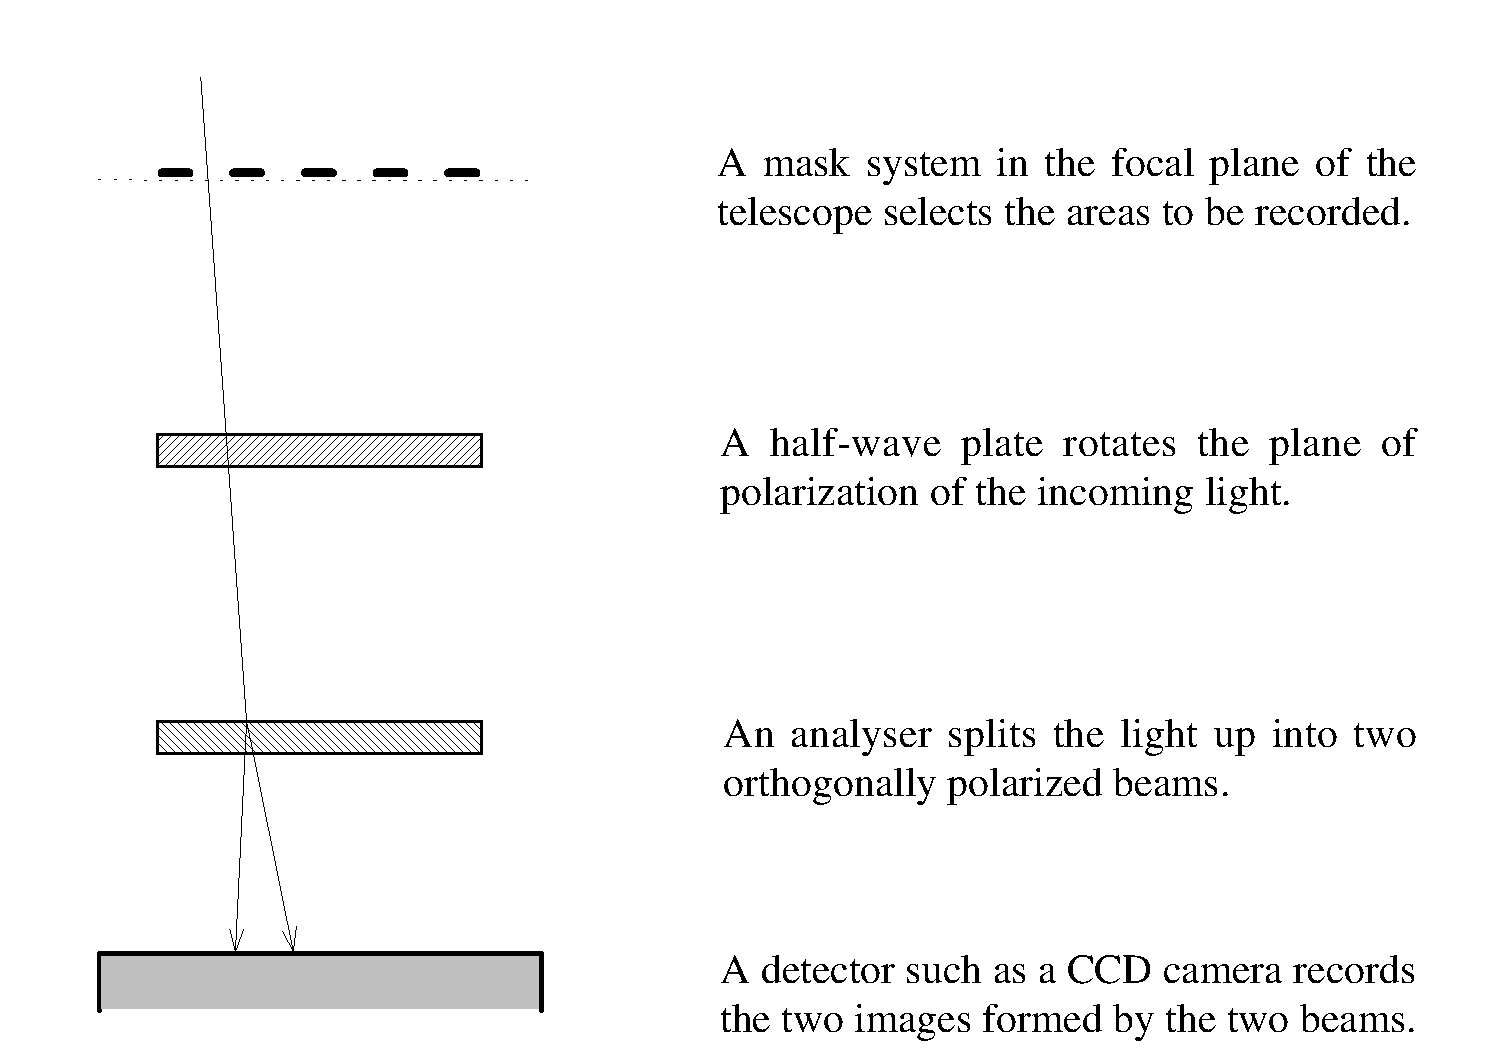
\includegraphics[clip,scale=0.5]{sun223_figures/optical.eps}
  \caption{The main optical components in a typical dual-beam imaging polarimeter.}
  \label{fig:optical}
  \end{center}
  \end{figure}
\end{latexonly}
\begin{htmlonly}
   \begin{quote}
   \begin{figure}[bhtp]
   \label{fig:optical}
   \includegraphics{sun223_figures/optical_htx.eps}
   \caption{The main optical components in a typical dual-beam imaging polarimeter.}
   \end{figure}
   \end{quote}
\end{htmlonly}

The heart of the polarimeter is the \emph{analyser}, which splits incoming
partially plane polarized light up into two beams; one (called the
ordinary, or $O$ ray) contains the component of the incoming light
which is polarized parallel to the axis of the analyser, and the other
(called the extraordinary, or $E$ ray) contains the component of the
incoming light which is polarized orthogonally to the axis of the
analyser. These two beams are recorded simultaneously on a suitable
detector such as a CCD. The advantage of this system over a single-beam
instrument (in which only one state of polarization is recorded on a
given exposure), is that variations in sky background between exposures
affect both states of polarization equally, and so can be eliminated.

In an imaging polarimeter, the two beams form two images on the detector,
displaced by some distance determined by the design of the instrument;
both images representing the same area of the sky. A \emph{masking system}
is used to prevent any overlap between the two images. In some
instruments this takes the form of a series of parallel, equally spaced
bars in the focal plane of the telescope (see Figure~\ref{fig:grids}). In
this case, the instrument is designed so that the displacement between
the two images formed by the $O$ and $E$ rays is perpendicular to the
bars, and equal in size to the width of a bar. Thus, the two images form
two inter-leaving sets of bars. There are several other systems (such as 
a mask containing only a single aperture), but the principle is the same.

\begin{latexonly}
  \begin{figure}[p]
  \begin{center}
  \includegraphics[clip,scale=0.8]{sun223_figures/grids.eps}
  \caption{An example of a masking system used in a dual-beam imaging polarimeter.}
  \label{fig:grids}
  \end{center}
  \end{figure}
\end{latexonly}
\begin{htmlonly}
   \begin{quote}
   \begin{figure}[hbtp]
   \label{fig:grids}
   \includegraphics{sun223_figures/grids_htx.eps}
   \caption{An example of a masking system used in a dual-beam imaging polarimeter.}
   \end{figure}
   \end{quote}
\end{htmlonly}

If the incoming light is only partially polarized, then at least two
exposures are required to estimate both the degree and the orientation of
the polarization, each exposure recording the intensity in two orthogonal
states of polarization as described above. The analyser axis is rotated
in steps of 45\dgs\ between these exposures. In practice, physically rotating
the analyser would result in the displacement between the $O$ and
the $E$ ray images also rotating. This would cause the images to overlap
on the detector and would make the data reduction process much harder (if
not impossible). For this reason, the analyser is usually left in a fixed
position, and the plane of polarization of the incoming light is rotated
instead. This is achieved by placing a \emph{half-wave plate} in
front of the analyser, and rotating it in steps of 22.5\dgs, resulting in
a rotation of the plane of polarization of 45\dgs. Using this scheme the
positions of the $O$ and $E$ ray images on the detector are unchanged.

The orientation of the plane of polarization of the incoming light is
measured relative to a fixed ``reference'' direction. The analyser axis
and the 0\dgs\ position of the half-wave plate are usually parallel to
this direction. 

\subsection{\label{SEC:OBS}\xlabel{theobservationalprocedure}The Observational Procedure}
At least two exposures are required to estimate the degree and
orientation of the polarization, taken with half-wave plate positions of
0\dgs\ and 22.5\dgs\ (see \hyperref{here}{appendix }{}{APP:POL}). For ease
of reference, these exposures are referred to here as $T_{0}$ and
$T_{22.5}$. The $O$ and $E$ ray images in $T_{0}$ measure the intensities
parallel and perpendicular to the reference direction. $T_{22.5}$ has an
effective analyser angle of 45\dgs\ (twice the half-wave plate angle) and
so measures the intensities at angles of 45\dgs\ and 135\dgs\ to the
reference direction

Usually, a further two exposures are taken at half-wave plate positions
of 45\dgs\ and 67.5\dgs\ (referred to here as exposures $T_{45}$ and
$T_{67.5}$). These provide some redundancy in the data and enable
internal consistency checks to be made during the data reduction stage.

These exposures are denoted by the letter $T$ to indicate that they are
\emph{target} exposures. In addition to these target exposures, some {\em
flat-field} exposures are also required. These are used to correct for
any spatial variation in the sensitivity of the system, and consist of
exposures of a photometrically flat surface. Ideally, the flat-field
source should be unpolarized. However, if the additional target exposures
$T_{45}$ and $T_{67.5}$ are taken, then a spatially constant polarization 
across the flat-field source can be corrected for during data reduction.
Since the polarization of the flat-field surface is rarely known to be
zero, these additional target exposures should always be taken. 

It is important that the flat-field has a good signal-to-noise ratio.
For this reason, it is common practice to take one or more flat-field 
exposures at each half-wave plate position, and stack them together into a 
single master flat-field (although it is not strictly necessary to use
different half-wave plate positions). Further discussion of the flat-fielding
procedure is given \hyperref{here}{in section }{}{SEC:DETCOR}. 

\subsection{The Data Reduction}
Several steps are involved in the production of a polarization map from
the raw exposures recorded by the detector. An over-view of these steps
is given here. Details of how they may be implemented in practice using
POLPACK are given in later sections of this document.

\subsubsection{\label{SEC:DETCOR}Corrections Related to the Detector}
These convert the raw data numbers measured by the detector into values
which are proportional to the combined sky and object intensity
transmitted by the analyser (plus noise of course). The details of these
corrections will depend on the nature of the detector. For a CCD camera,
they will usually involve at least flat-fielding, and de-biassing. 

Flat-fielding is worthy of some extra discussion, since it can be
complicated by the presence of the polarimeter in the light path. The
purpose of flat-fielding is to ensure that there are no spatial
variations in the sensitivity of the detector. This is normally achieved
by taking images of a photometrically flat surface such as the inside of
the observatory dome, or the twilight sky\footnote{In the near infra-red
flat-fields are normally taken on the night sky which at these wavelengths
is bright enough to give a good signal to noise ratio.}. Since the
brightness of this surface is constant, any variations in the recorded
image (the ``flat-field'' image) must be due to variations in the
sensitivity of the detector. These variations can then be removed from the
target observation by dividing every pixel value in the target image by
the corresponding pixel value in the flat-field image.

Introducing a polarimeter into the light path can complicate this if the
flat-field is taken in polarized light (such as is produced by reflective
surfaces in the dome, or by light scattering in the atmosphere). In this
case the intensity of the light reaching the detector will not be
constant across the field, but will depend on the polarization. 

If the polarization of the flat-field is non-zero and spatially constant,
then the $O$ and $E$ ray flat-field images will have different mean
values (visible as sharply defined dark and light areas in the flat
field). If such a flat-field is used to correct the target exposures,
then the different mean values in the flat-field will result in an
apparent difference in sensitivity between the two channels of the
polarimeter (known as the ``F-factor''). Such a difference in sensitivity
can be corrected for when calculating the polarization if the additional
target exposures \hyperref{$T_{45}$ and $T_{67.5}$}{$T_{45}$ and
$T_{67.5}$ (see section }{)}{SEC:OBS} are available. 

\emph{Note, the same flat-field should be used to flat-field all target
exposures, irrespective of half-wave plate position.}

A mathematical description of the flat-fielding and F-factor corrections
is given \hyperref{here}{in appendix }{}{APP:FFCOR}.

\subsubsection{Extraction of the $O$ and $E$ Ray Images}
Each exposure contains two images of the same area of the sky: the $O$
and the $E$ ray images. Once any detector corrections have been applied,
these images need to be identified and extracted into two separate arrays for
further processing.

\begin{latexonly}
  \vspace{5mm}
  \begin{figure}[htbp]
  \begin{center}
  \includegraphics[clip,scale=0.5]{sun223_figures/extract.eps}
  \caption{Extraction of the $O$ and $E$ ray images.}
  \label{fig:extract}
  \end{center}
  \end{figure}
\end{latexonly}
\begin{htmlonly}
   \begin{quote}
   \begin{figure}[hbtp]
   \label{fig:extract}
   \includegraphics{sun223_figures/extract_htx.eps}
   \caption{Extraction of the $O$ and $E$ ray images.}
   \end{figure}
   \end{quote}
\end{htmlonly}

\subsubsection{Image Alignment}
The arrays holding the extracted $O$ and $E$ ray images now need to be
aligned so that the same pixel in each array corresponds to the same
position on the sky. This can usually be achieved by aligning stars
within the arrays.

\subsubsection{Sky Subtraction}
The intensity of the background night sky now needs to be estimated and
subtracted from each of the aligned arrays. The sky may be polarized, and
so this needs to be performed independently within each of the aligned arrays.

\subsubsection{Estimation of the Stokes Parameters}
The \emph{Stokes parameters} $I$, $Q$ and $U$ are all measures of intensity,
and together provide a useful description of the polarization of the object
being studied. Since $I$, $Q$ and $U$ all have the same units, this
description is generally easier to use than the more obvious description
given by the degree of polarization and the orientation of the plane of
polarization. The mathematical connection between the Stokes parameters 
and the sky-subtracted intensities is described \hyperref{here}{in
appendix }{}{APP:POL}. The output from this stage of the reduction process
is a \emph{Stokes vector} (\emph{i.e.} a set of $I$, $Q$ and $U$ values) for each
measured pixel on the sky.

\subsubsection{Binning of the Stokes Parameters}
One consequence of the fact that the Stokes parameters $I$, $Q$ and $U$
are all measures of intensity, is that they can be binned spatially. This
not only produces less confusing polarization maps (due to the reduced
number of measurements), but also improves the signal-to-noise ratio.

\subsubsection{Calculation of the Degree and Orientation of the Polarization}
The use of Stokes parameters to describe polarization has mathematical
advantages, but is not easy to represent in a graphical manner. For human
interpretation therefore, polarization is usually described by the degree
of polarization, $p$, (\emph{i.e.} the ratio of polarized to total intensity),
and the orientation of the plane of polarization, $\theta$. Note,
$\theta$ is the angle between the plane of polarization and the reference
direction of the polarimeter. To convert this to a position angle on the
sky, the position angle of the reference direction must be known. The
simplest way to derive these parameters from the Stokes parameters is as
follows:

\begin{myquote}
\begin{eqnarray*}
  I_{p} & = & \sqrt{ Q^{2} + U^{2} } \\
  p & = & I_{p}/I \\ \\
  \theta & = & 0.5.\arctan (U/Q)
\end{eqnarray*}
\end{myquote}

where $I_{p}$ is the \emph{polarized intensity}. However, the estimation
of $p$ is complicated by the non-symmetric noise statistics produced by
squaring and adding $Q$ and $U$. For low polarizations, the squaring of
the noise will tend to shift the mean of the distribution of $p$ to
higher values, thus resulting in an over-estimation of $p$. The use of
the following expression for $I_{p}$ reduces the effect of this
statistical bias:

\begin{myquote}
\begin{eqnarray*}
  I_{p} & = & \sqrt{ Q^{2} + U^{2} - \sigma^{2}} \\
\end{eqnarray*}
\end{myquote}

where $\sigma^{2}$ is the variance on $Q$ or $U$ (which are assumed
equal). A description of the statistical behaviour of polarization
parameters is given by Serkowski (\emph{Advances in Astronomy and
Astrophysics}, ed. Z. Kopal, Academic Press, New York, London (1962),
\textbf{1}, 304).

\subsubsection{Display of the Final Polarization Data}
The final polarization parameters are usually presented graphically in
the form of a \emph{polarization map} (see the first page of this document
for an example). Each measurement is represented as a vector parallel to
the plane of polarization. The length of the vector is proportional to
the degree of polarization, which varies from 0\% to 100\%. The Stokes
vectors can be binned to reduce the number of vectors in the map to a
manageable number. The map is often overlayed on a total intensity image
or contour map of the object to emphasize any correlation between the
visual appearance of the object and the morphology of the polarization
map.

\section{\xlabel{datareductionusingpolpack}Data Reduction Using POLPACK}
This section gives a detailed description of the steps involved in using
POLPACK to produce a vector map from dual-beam polarimetry data. It is
assumed that the data conforms to the model outlines in the previous
section. An over-view of the data reduction process is given in
Figure~\ref{fig:dataflow}.

\begin{latexonly}
  \begin{figure}[htpb]
  \begin{center}
  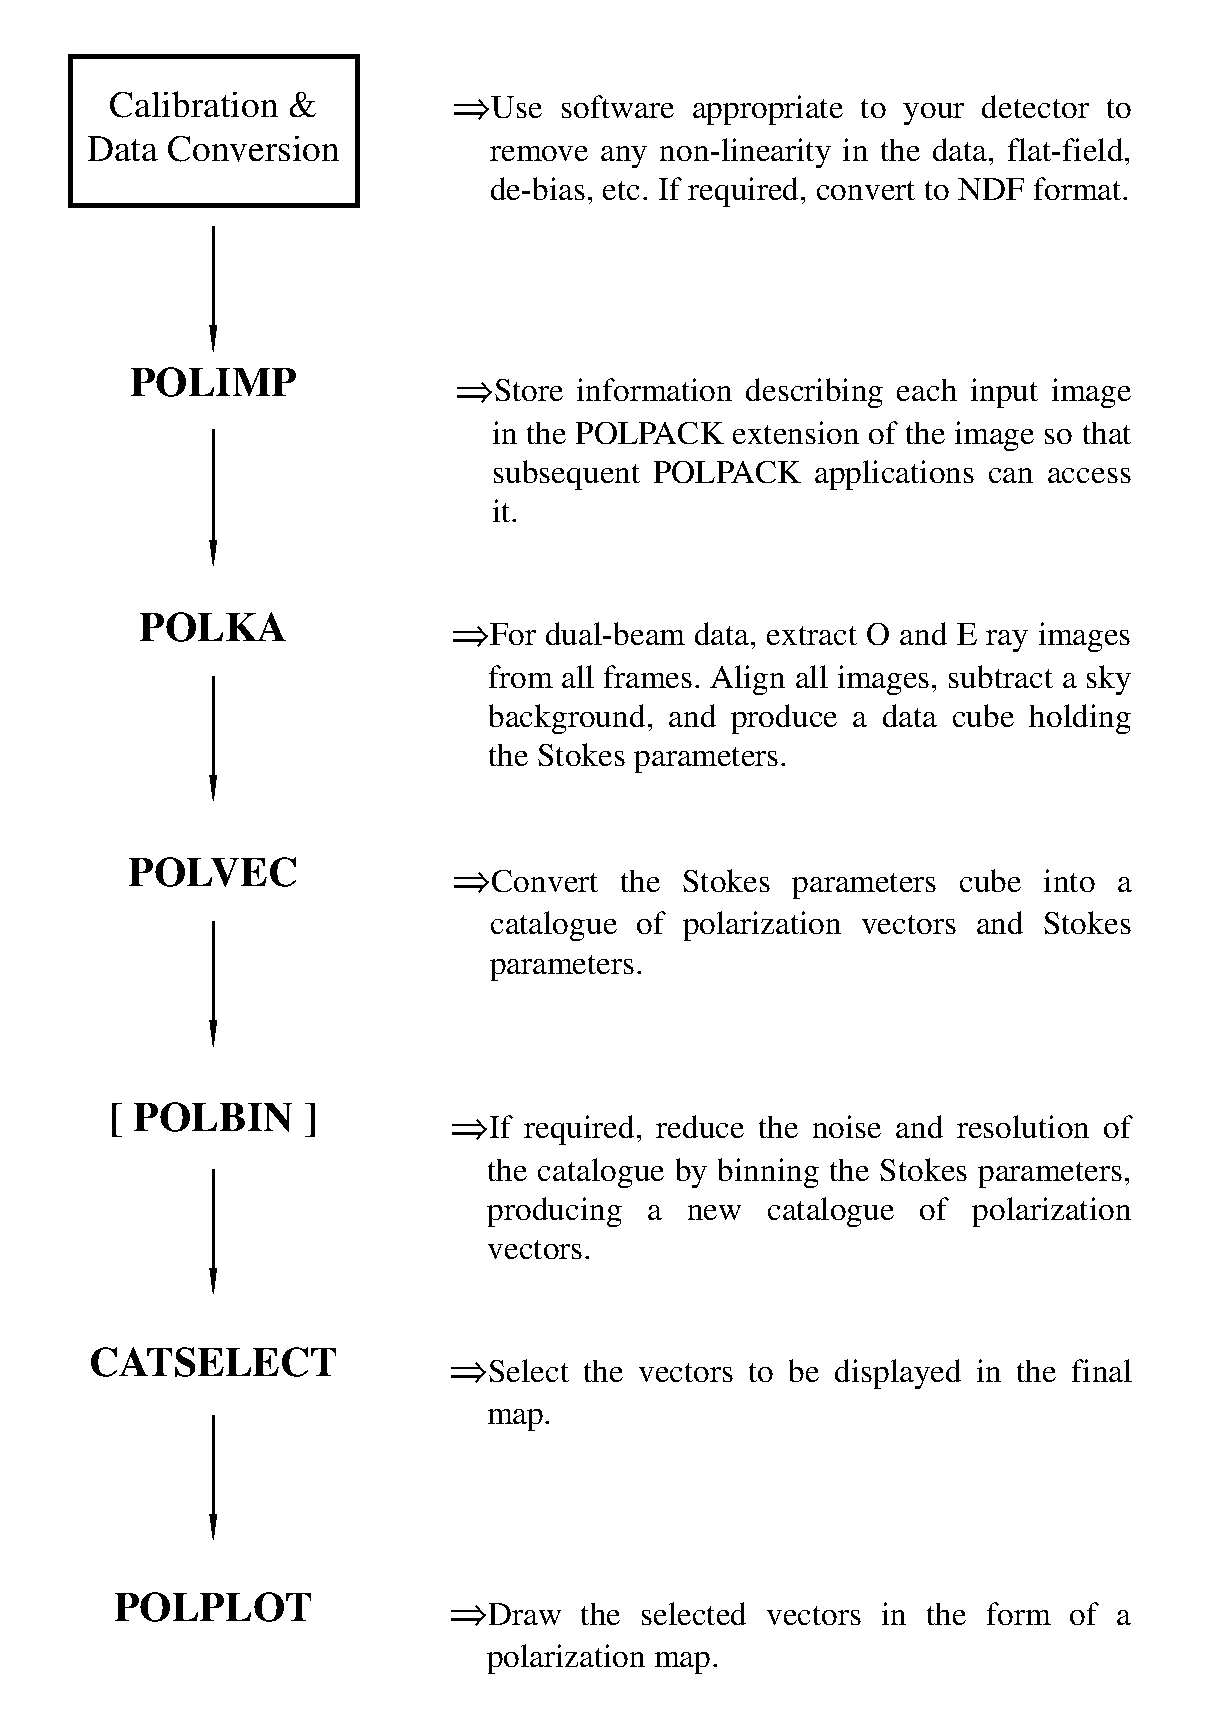
\includegraphics[clip,scale=0.7]{sun223_figures/dataflow.eps}
  \vspace{4mm}
  \caption{The main steps in the production of a polarization map.}
  \label{fig:dataflow}
  \end{center}
  \end{figure}
\end{latexonly}
\begin{htmlonly}
   \begin{quote}
   \begin{figure}[bhtp]
   \label{fig:dataflow}
   \includegraphics{sun223_figures/dataflow_htx.eps}
   \caption{The main steps in the production of a polarization map.}
   \end{figure}
   \end{quote}
\end{htmlonly}

All POLPACK applications use standard Starlink subroutine libraries for
accessing parameters, producing graphics, reporting errors, \emph{etc}. They
therefore look and feel very similar to applications in other Starlink
packages such as KAPPA and CCDPACK. The following sections in
\xref{SUN/95}{sun95}{} should therefore be consulted for general
information about these issues:

\begin{itemize}
\item ``\xref{Parameters}{sun95}{se_param}''
\item ``\xref{Graphics Devices and Files}{sun95}{se_graphdev}''
\item ``\xref{Data Structures}{sun95}{se_datastr}''
\item ``\xref{NDF Sections}{sun95}{se_ndfsect}''
\item ``\xref{NDF History}{sun95}{se_ndfhistory}''
\item ``\xref{Graphics Database}{sun95}{se_agitate}''
\item ``\xref{Procedures}{sun95}{se_procedures}''
\end{itemize}

\subsection{\label{SEC:CONVERT}\xlabel{formatconversion}Format Conversion}
The first step is to ensure that your data files are in a format which
POLPACK can process. The native data format used by POLPACK is the 
Starlink \xref{NDF}{sun33}{} format (note, NDF structures are usually stored in
files with a file type of \verb+.sdf+). If your data is already in this
format, then you can proceed immediately to the next step. Otherwise,
you have two options:

\begin{enumerate}

\item You can explicitly convert your data files into NDF format at the
beginning, and use the NDF versions there-after. The \xref{CONVERT}{sun55}{} 
package {\latexonly (see SUN/55)} provides facilities for converting to and
from most common astronomical data formats. For instance, if your data is
in the form of a set of FITS files, you could use commands similar to the
following to convert them into NDFs:

\begin{myquote}
\begin{verbatim}
% convert
% fits2ndf "*.fit" "*"
\end{verbatim}
\end{myquote}

Note that the \text{\%} represents the C-shell prompt and should not be typed.
The first command initialises the commands required to use the CONVERT
package. The second command converts all FITS files with a file type of
\verb+.fit+ within the current directory, into equivalent NDFs with the
same file names, but a file type of \verb+.sdf+\footnote{The double quotes
are needed to prevent the asterisks being expanded by the shell. The
expansion of these file templates is performed internally, within
fits2ndf.}. The \verb+.sdf+ files can then be given as inputs to
any application from POLPACK, CCDPACK or KAPPA.

\item Alternatively, you can rely on the facilities of the NDF library to perform
automatic on-the-fly data conversions as and when necessary. Using this
technique, POLPACK, CCDPACK and KAPPA all appear to process your data files
directly without you needing to do any explicit data conversion. All you
need to do to enable these facilities is to initialise the CONVERT
package using the single command:

\begin{myquote}
\begin{verbatim}
% convert
\end{verbatim}
\end{myquote}

If you adopt this approach, you may still see references to ``NDFs''
appearing on the screen. There is usually no significance in the use of
the term ``NDF'' in this context (unless there are indications to the
contrary), and you should understand these as referring to your own
non-NDF data files.

\end{enumerate}

\subsection{\label{SEC:CCDPACK}Corrections for Instrumental Effects}
POLPACK expects your data to be calibrated so that the pixel values are
proportional to the analysed intensity. You should therefore correct your
data for any known instrumental effects such as non-linearity, variation
of sensitivity across the detector, zero point offsets, \emph{etc}, before
proceeding to use POLPACK. The details will obviously depend on your
detector, but if you are using a CCD camera, then \xref{CCDPACK}{sun139}{} 
{\latexonly (see SUN/139)} will usually be able to perform these corrections.

If target exposures are available at half-wave plate positions of
45.0\dgs\ and 67.5\dgs\ (as well as 0\dgs\ and 22.5\dgs), then POLPACK can
make corrections for the following effects when calculating the Stokes
vectors:

\begin{enumerate}
\item Differences in exposure times between the target exposures
\item A constant difference in sensitivity between the $O$ and $E$ ray
channels.
\end{enumerate}

These effects therefore do not need to be calibrated out of the raw data.

One aspect of calibration common to all detectors is flat-fielding. If
your flat-fields are obtained in polarized light (such as produced by
reflection or scattering, for instance), then the mean signals measured
in the $O$ and $E$ ray images will be different. When such a flat-field
is used to calibrate your target exposures, these different mean levels
will introduce an apparent difference in sensitivity between the $O$ and
$E$ ray channels. If the \emph{same} flat-field is used for all target
exposures, then this difference in sensitivity will be constant and can
be removed while calculating the Stokes parameters (provided you have
target exposures at half-wave plate positions of 0, 22.5, 45 and 67.5
degrees). \hyperref{Go here for}{Appendix }{ contains}{APP:FFCOR} a
mathematical description of the flat-fielding process, and the
corrections applied by POLPACK when calculating the Stokes parameters.

\emph{Do not forget to use the same flat-field to correct \textbf{all} target
exposures}. This will usually be a master flat-field formed by co-adding
several individual flat-field exposures. This reduces the noise in the
master flat-field. This is important for two reasons:

\begin{enumerate}
\item Any noise in the flat-field gets passed directly into the final results.
\item Any noise in the flat-field appears in each of the flat-fielded
intensity images, resulting in a degree of correlation between the noise in 
these images. This can cause any variance estimates for the final
polarization parameters (see next paragraph) to be wrong. This is because 
the variance calculations assume that there is no correlation between the 
noise in different images. 
\end{enumerate}

Another aspect of instrumental calibration is the estimation of the
uncertainty on every pixel value. If you know the noise characteristics
of your detector, you may be able to store this information with your
data in the form of an NDF \emph{VARIANCE component}. This is an array
holding an estimate of the variance at every pixel in your data. If
present, POLPACK will process this information to obtain estimates of the
uncertainty in the final polarization parameters. If you use CCDPACK to
calibrate your data, then the \xref{DEBIAS}{sun139}{DEBIAS} application
can be used to create a VARIANCE component.

\subsection{\label{SEC:START}\xlabel{startup}Starting up POLPACK}

The applications within POLPACK are made available from the C shell using the 
command:
\begin{myquote}
\begin{verbatim}
% polpack
\end{verbatim}
\end{myquote}

This command must be issued before attempting to use any POLPACK
applications. 

\subsection{\label{SEC:IMPORT}Importing Header Information}
POLPACK needs to know certain items of header information about each of
the supplied data files. These include the half-wave plate position, the
orientation of the reference direction, \emph{etc}. Different instruments may
store this information in different ways, and for this reason, POLPACK
includes an application which finds the required items of information and
stores them away in a standard place within the data file from where the
other POLPACK applications can extract them when needed. This standard
place is known as the ``POLPACK extension''. The process of copying this
information from its original, instrument specific location, into the
POLPACK extension is known as ``importing'' the data, and is performed by
the \htmlref{POLIMP}{POLIMP} application\footnote{Once imported, the POLPACK
extension is propagated through the entire data reduction sequence, with
new items being added at various points to describe the intermediate
stages of processing.}, or the \htmlref{POLEXT}{POLEXT} application (if
you have no FITS headers available).

You tell POLIMP where to find each required item of information by
supplying it with a ``control table''. This is a text file containing a
line for each item of information to be imported into the POLPACK
extension. Each such item has a name by which other POLPACK applications
refer to it (these are described \hyperref{here}{in
appendix }{}{APP:POLEXT}). As well as the name of a POLPACK extension
item, each line of the control table should contain a description of where to
obtained the corresponding value. This description is given in terms of
FITS keywords. For instance, the line

\begin{myquote}
\begin{verbatim}
   WPLATE HWPANG
\end{verbatim}
\end{myquote}

tells POLIMP to find the value of the FITS keyword \verb+HWPANG+ and
store it as item ``WPLATE'' in the POLPACK extension (this is the
half-wave plate position angle).

If your data are supplied in the form of a set of FITS files, then the
\verb+HWPANG+ value would simply be obtained from the primary header. If your
data is supplied in the form of a set of NDF structures, then the value
would be read from the FITS extension in the NDF structure (which should
have been created by the data acquisition system). For other data formats,
the origin of the keyword value depends on how the data conversion is
performed. \xref{SUN/55}{sun55}{} contains details of how FITS keywords
are created from foreign data files.

The POLIMP control table also allows POLPACK extension items to be
derived from one or more FITS keyword values, combined together to form a
Fortran-like mathematical expression. For instance, this may be useful if
the FITS keyword uses a different set of units, or has a different sign
convention. When used in this way, each FITS keyword must be ``declared''
earlier in the control table. This declaration tells POLIMP what sort of
data values the keyword can take. For instance:

\begin{myquote}
\begin{verbatim}
   _REAL  ROTA
   ANGROT 57.29578*ROTA
\end{verbatim}
\end{myquote}

converts the value of the FITS keyword \verb+ROTA+ from radians to
degrees, and assigns the result to the item ANGROT in the POLPACK extension.
The first line informs POLIMP that the keyword \verb+ROTA+ should be
treated as a single precision floating point value. The recognized data
types are:

\begin{quote}
\begin{description}
\item[\texttt{\_BYTE}]		- Single byte signed integer values.
\item[\texttt{\_CHAR}]		- Character strings.
\item[\texttt{\_DOUBLE}]       	- Double precision floating point values.
\item[\texttt{\_INTEGER}]	- Single precision integer values.
\item[\texttt{\_REAL}]		- Single precision floating point values.
\item[\texttt{\_WORD}]		- Two byte signed integer values.
\end{description}
\end{quote}

See the description of the \htmlref{POLIMP}{POLIMP} application for
further details of the syntax of the control table.

There is also a \htmlref{POLEXP}{POLEXP} application which reverses the 
importing process. It copies the information stored in the POLPACK
extension into named FITS keywords. The primary purpose of POLEXP is 
to allow the automatic format conversion facilities of the NDF library to
convert a POLPACK NDF structure back into a foreign data file.
It is generally not necessary for users to call POLEXP explicitly. 

The \htmlref{POLEXT}{POLEXT} application allows the contents of the
POLPACK extension to be set to explicit values supplied by the user. This
can be useful if your data does not contain any FITS headers. POLEXT will
also list the contents of the POLPACK extension. If your data is stored
in NDF format, you can also use the \xref{\texttt{hdstrace}}{sun102}{}
command to list the contents of the NDF extension. For instance, to check
the contents of the POLPACK extension in the NDF \verb+partproc.sdf+, do:

\begin{myquote}
\begin{verbatim}
   % hdstrace partproc.more.polpack
\end{verbatim}
\end{myquote}

\subsection{Creation of Stokes Parameters}
The creation of Stokes vectors from the calibrated, imported 
target exposures involves the following steps:

\begin{itemize}
\item The extraction of the $O$ and $E$ ray images in each target
exposure into separate files.
\item The alignment of all these separated $O$ and $E$ ray images, so
that a given pixel position corresponds to the same place on the sky in
all images.
\item The subtraction of a sky background from each $O$ and $E$ ray image.
\item The calculation of the Stokes vectors from these sky-subtracted
images.
\end{itemize}

The first three of these steps can be performed using applications from
KAPPA and CCDPACK, and the final step is performed by the POLPACK
application \htmlref{POLCAL}{POLCAL}. However, this is a fairly involved
process since the available applications are somewhat low-level. For this
reason, POLPACK includes a tool called \htmlref{POLKA}{POLKA} which
simplifies the process. POLKA is effectively a script which calls the
KAPPA, CCDPACK and POLPACK applications required to perform all four of
the steps listed above\footnote{The final step - calculating the Stokes
parameters - is optional. This allows POLKA to be used as a general
purpose image alignment tool for non-polarimetric data.}. While some
options are provided to allow the user to customise the exact recipe
used, POLKA does not provide as much versatility or control over the
processing as would be available if the individual applications were
called ``by hand''. If you hit a problem which POLKA cannot handle, then
you may need to adopt this alternative approach.

POLKA requires you to identify the following features within the supplied
images:

\begin{itemize}
\item The areas containing the $O$ and $E$ ray images.
\item The sky areas.
\item Any star-like features which can be used to align the images.
\end{itemize}

A Graphical User Interface (GUI) is created for this purpose, including
an image display area in which any of the input images may be displayed,
and controls to select any of the above features (see Figure
~\ref{fig:polka}). Note, if you find the image display area uncomfortably
small, it can be made larger by assigning a suitable value to the DPI
parameter when POLKA is started. Once the required features have been
supplied, POLKA commences the processing of the supplied data frames.
This may take a significant length of time depending on your hardware,
and the size and number of your images. A window displays the progress
being made during this phase.

\begin{latexonly}
  \begin{figure}[htpb]
  \begin{center}
  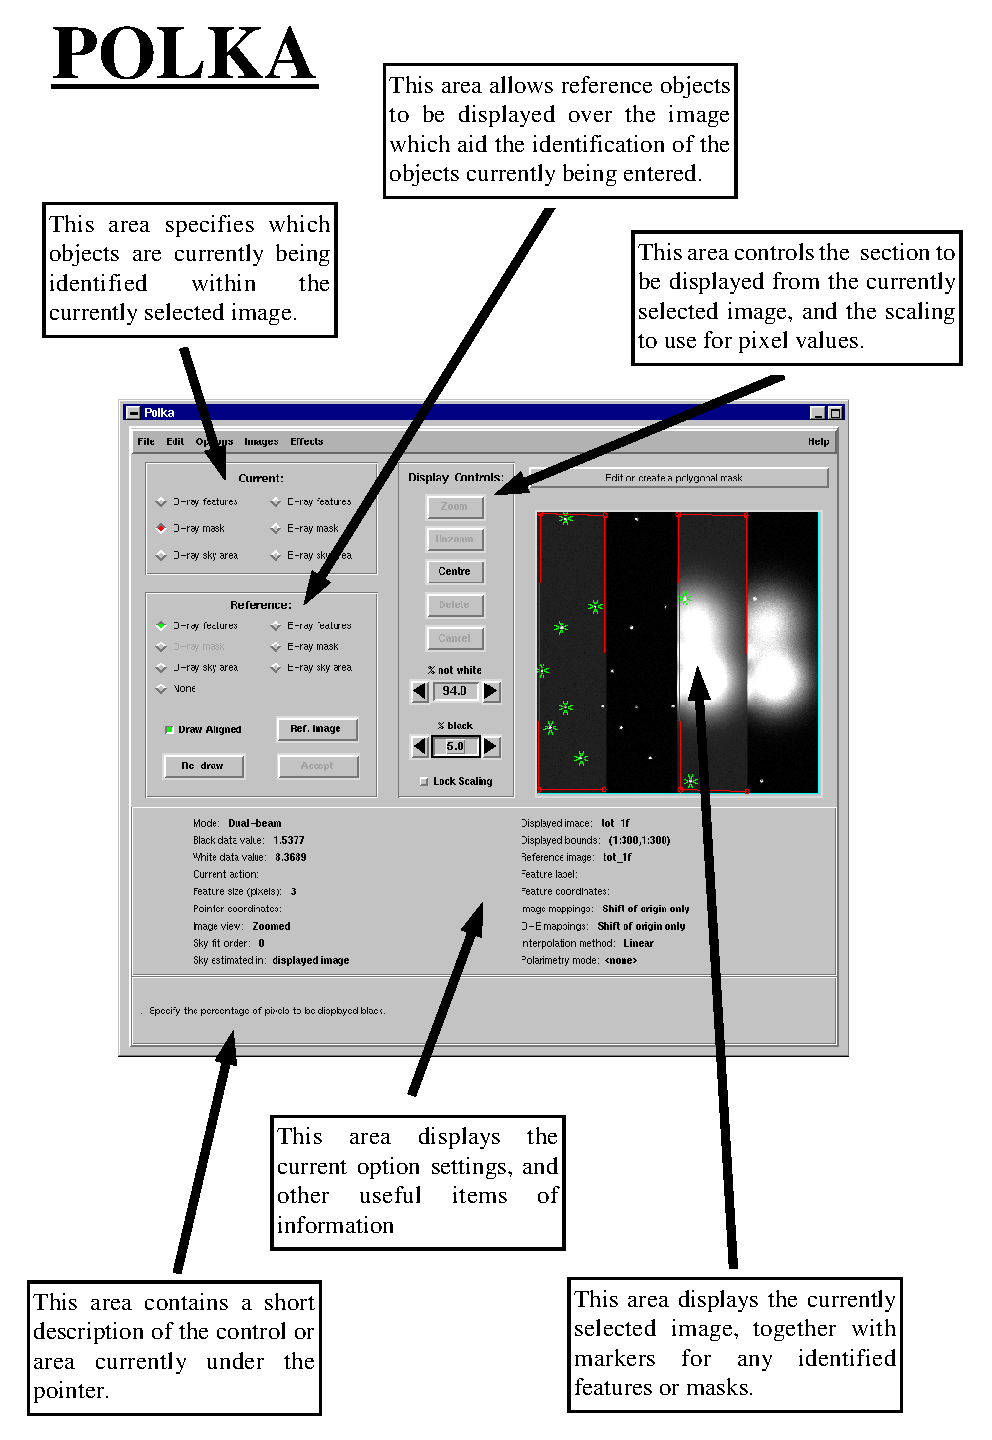
\includegraphics[clip,scale=0.9]{sun223_figures/polka.eps}
  \vspace{4mm}
  \caption{The Graphical User Interface presented by POLKA.}
  \label{fig:polka}
  \end{center}
  \end{figure}
\end{latexonly}
\begin{htmlonly}
   \begin{quote}
   \begin{figure}[bhtp]
   \label{fig:polka}
   \includegraphics{sun223_figures/polka_htx.eps}
   \caption{The Graphical User Interface presented by POLKA.}
   \end{figure}
   \end{quote}
\end{htmlonly}

Once complete, a 3D cube is created in which the x-y plane corresponds to
pixel positions within the extracted, aligned intensity images. Each
plane in the cube contains a single Stokes parameter. The lowest plane is
always the total intensity. The other planes contain either Q and U for
linear polarization, or V for circular polarization. In addition, the
separate intensity images on which the Stokes parameters were based may
be saved once the processing is complete.

The POLKA application has many parameters. The values used for some of
these may be changed from within the GUI. However, some may not be
changed and should be assigned appropriate values when invoking POLKA.
Of these, the most important will usually be:

\begin{quote}
\begin{description}
\item [IN]	- A list of the input target frames. These should have been
calibrated and imported. The list may be supplied in several forms
(described \hyperref{here}{in section }{}{SEC:GRPEXP}).
\item [MODE]	- Indicates what sort of polarization you are measuring. It 
can be ``CIRCULAR'' or ``LINEAR''.
\item [OUT\_E]	- A list of the output images to receive the extracted,
aligned, sky-subtracted $E$ ray images. If a null value (!) is supplied, 
these images are not saved.
\item [OUT\_O]	- This is like OUT\_E, but refers to the $O$ ray images
instead of the $E$ ray images.
\item [OUT\_S]	- The name of the output cube to receive the Stokes
parameters. If a null value (!) is supplied, no Stokes parameters are
created.
\item [POL]	- This should be set to FALSE if you want to use POLKA as a
general purpose image alignment tool for non-polarimetric data. If this
is done, the aligned, sky-subtracted images should be specified using parameter
OUT (parameters OUT\_S, OUT\_E and OUT\_O are then not used). In this mode,
the supplied images are treated like $O$ ray images, and the controls
related to the $E$ ray images are disabled.
\item [SKYFRAMES] - POLKA provides two methods of sky subtraction. If a
list of frames is supplied for parameter SKYFRAMES, then these frames are
subtracted pixel-by-pixel from the target intensity frames. If a null
parameter value (!) is supplied for SKYFRAMES, then you must use the GUI to
identify areas of sky within each of the input target frames. A smooth
surface is then fitted to these areas and used as the sky background.

\end{description}
\end{quote}

A separate guide is available describing POLKA in detail. This guide
contains a step-by-step tutorial, detailed descriptions of 
each control in the GUI, answers to some common questions, \emph{etc}. It may be
accessed using the \verb+Help+ menu within the GUI. When POLKA is
activated, the tutorial is automatically displayed in a WWW browser (this
may be disabled using the STARTHELP parameter when running POLKA). If you
are new to POLKA, it is  a good idea to work your way through the
tutorial first.


\subsection{\label{SEC:DISP}Displaying the Results}
Linear polarimetry results are usually expressed in terms of the percentage
polarization and the orientation of the plane of polarization (see
\hyperref{here}{appendix }{}{APP:POL}). Vectors may be used to represent
these quantities graphically. The following POLPACK applications can be
used to produce a map of vectors describing the polarization at different
points on the sky:

\begin{quote}
\begin{description}
\item [\htmlref{POLVEC}{POLVEC}] - This converts a 3D cube containing Stokes parameters
(such as produced by POLKA or POLCAL) into a catalogue containing the
following columns:

\begin{quote}
\begin{description}
\item [X] - X pixel coordinates within the supplied cube.
\item [Y] - Y pixel coordinates within the supplied cube.
\item [I] - Total intensity.
\item [Q] - Stokes parameter Q.
\item [U] - Stokes parameter U.
\item [P] - Percentage polarization.
\item [ANG] - The anti-clockwise angle from the X pixel axis to the plane of 
polarization, in degrees.
\end{description}
\end{quote}

For circular polarimetry, the Q and U columns are replaced by a single V
column. If variance information is available (see
\hyperref{here}{section }{}{SEC:CCDPACK}) then columns are also produced
holding the standard deviations associated with each of the above
quantities (except X and Y). The catalogue contains a single row for each
pixel in the x-y plane of the supplied cube.

POLVEC can also produce a set of 2D images holding the above quantities.

\item [\htmlref{POLBIN}{POLBIN}] - This accepts a catalogue containing Stokes
parameters as input (such as produced by POLVEC), and creates a new
output catalogue in the same format, but containing fewer rows (\emph{i.e.}
fewer polarization vectors). The output catalogue is formed by binning the
Stokes vectors in the input catalogue within a grid of equally sized
rectangular bins. Corresponding values for the P and ANG columns are
calculated on the basis of the binned Stokes parameters.

\item [\htmlref{POLPLOT}{POLPLOT}] - This displays a map of polarization 
vectors, obtained from a catalogue produced by POLVEC or POLBIN. If the
map is drawn over an existing picture, then the vectors can be aligned
with the previously displayed picture.

\end{description}
\end{quote}

Since the polarization parameters are stored in a catalogue, the
\xref{CURSA}{sun190}{} package {\latexonly (see SUN/190)} can be used to
examine and manipulate them. One particularly useful facility within
CURSA is the \xref{CATSELECT}{sun190}{SELECT} application, which
allows rows within a catalogue to be selected on the basis of an
arbitrary mathematical expression. For instance the following commands
create a new catalogue called \verb+selcat.FIT+ which contains all the
vectors from \verb+bincat.FIT+ for which the polarization is less than
30\% and has a standard deviation less than 5\%:

\begin{myquote}
\begin{verbatim}
   % cursa
   % catselect catin=bincat catout=selcat norejcat seltyp=e "expr='p<30 & dp<5'"
\end{verbatim}
\end{myquote}

The \xref{XCATVIEW}{sun190}{XVIEW} application allows you to examine the
data in a catalogue, using a Graphical User Interface to control the
operation and display the results.

A typical recipe for using the above applications (together with KAPPA)
would involve the following steps:

\begin{enumerate}

\item Convert the 3D NDF in file \verb+cube.sdf+ containing Stokes vector 
(created by POLKA) into a catalogue stored in file \verb+cat.FIT+:

\begin{myquote}
\begin{verbatim}
   % polvec cube cat
\end{verbatim}
\end{myquote}

\item Bin the catalogue to reduce the noise and decrease the density
of vectors in the final map. The bins used are 8 by 8 pixels (measured in
the x-y plane of the Stokes parameter NDF \verb+cube.sdf+), and the
Stokes parameters are combined using a median. The binned catalogue is
stored in file \verb+bincat.FIT+:

\begin{myquote}
\begin{verbatim}
   % polbin cat bincat 8 method=med
\end{verbatim}
\end{myquote}

\item Create a new catalogue (in file \verb+selcat.FIT+) containing just
the vectors with polarizations of less than 50\% and standard deviations of
less than 5\%:

\begin{myquote}
\begin{verbatim}
   % cursa
   % catselect catin=bincat catout=selcat norejcat seltyp=e "expr='p<50 & dp<5'"
\end{verbatim}
\end{myquote}

\item \label{STEP:DEVICE} Start up KAPPA, and then select the graphics 
device and the image display device (both are set to an X windows display 
in this example):
\begin{myquote}
\begin{verbatim}
   % kappa
   % gdset xwindows
   % idset xwindows
\end{verbatim}
\end{myquote}

\item Clear the screen:
\begin{myquote}
\begin{verbatim}
   % gdclear
\end{verbatim}
\end{myquote}

\item \label{STEP:PICDEF} Create a ``picture'' to contain a grey-scale display of the total
intensity. A picture is an area of the screen in which subsequent graphics
will appear. The one we create here is centred on the screen and occupies
three quarters of its height and width. This leaves a border available
for annotation round the display:
\begin{myquote}
\begin{verbatim}
   % picdef mode=cc fraction=0.75
\end{verbatim}
\end{myquote}

\item \label{STEP:DISPLAY} Display the total intensity image contained in the bottom plane of 
the Stokes vector cube, and ensure it is displayed with the standard 
monochrome colour table:
\begin{myquote}
\begin{verbatim}
   % display "cube(,,1)" mode=per percentiles="[5,95]"
   % lutgrey
\end{verbatim}
\end{myquote}

\item \label{STEP:PICLIST} Re-select the ``base picture''. This is a
picture which corresponds to the whole screen. We need to do this because
output from graphics applications such as POLPLOT is usually restricted
to the current picture. At the moment, the current picture is the one
created by PICDEF above which contains the grey-scale image. We want the
key produced by POLPLOT to appear outside this picture. We therefore need
to select the base picture so that POLPLOT has room for the key within
the current picture:
\begin{myquote}
\begin{verbatim}
   % piclist picnum=1
\end{verbatim}
\end{myquote}

\item \label{STEP:POLPLOT} Display the vector map, retaining the existing picture so that the
vectors appear in alignment with the previously displayed total intensity
image. The vectors are drawn in blue. A default scale will be used for the 
vectors, but this can be over-ridden if necessary by specifying a value for
parameter \htmlref{VSCALE}{POLPLOT}:
\begin{myquote}
\begin{verbatim}
   % polplot selcat noclear "style='colour(vect)=blue'"
\end{verbatim}
\end{myquote}

\end{enumerate}

The above basic recipe can be modified in many ways. For instance:

\begin{itemize}

\item If you want to display only a sub-section of the map, specify the
sub-section in step \ref{STEP:DISPLAY} by including bounds for the
first and second axes of input cube. For instance, to restrict the
display to X pixel coordinates 50 to 100, and Y pixel coordinates 300 
to 380, do:

\begin{myquote}
\begin{verbatim}
   % display "cube(50:100,300:380,1)" mode=per percentiles="[5,95]"
\end{verbatim}
\end{myquote}

\item If you do not want the vectors to be overlaid on a total
intensity image, then omit steps \ref{STEP:PICDEF} and
\ref{STEP:DISPLAY}, and remove the \verb+noclear+ setting from the
POLPLOT command line in step \ref{STEP:POLPLOT}.

\item If you want the vectors overlaid on a contour map instead of a
grey-scale image, replace step \ref{STEP:DISPLAY} with:

\begin{myquote}
\begin{verbatim}
   % contour "cube(,,1)" mode=per percentiles="[90,93,96,99]" noaxes nokey
\end{verbatim}
\end{myquote}

\item If you want your output in the form of a PostScript file, there is
an extra step. This is because graphics applications such as DISPLAY,
CONTOUR, POLPLOT, \emph{etc}, produce separate output PostScript files which
then need to be combined into a single file using the 
\xref{\texttt{psmerge}}{sun164}{} command. In step \ref{STEP:DEVICE},
specify the device as \verb+epsf_l+ (Encapsulated PostScript, landscape
mode) instead of \verb+xwindows+. The first graphics applications to be
run will then write its output to the file \verb+gks74.ps+, and
subsequent graphics applications will write their output to files
\verb+gks74.ps.1+, \verb+gks74.ps.2+, \emph{etc}\footnote{The sequence number
added to the end of the file name is always one higher than in any
existing files.}. To produce a contour map with overlaid vectors, replace
steps \ref{STEP:DISPLAY} and \ref{STEP:POLPLOT} with:

\begin{myquote}
\begin{verbatim}
   % rm gks74.ps*
   % contour "cube(,,1)" mode=per percentiles="[90,93,96,99]" noaxes nokey
   % mv gks74.ps.1 contour.ps
   % polplot selcat noclear 
   % mv gks74.ps.1 polplot.ps
   % psmerge polplot.ps contour.ps > total.ps
\end{verbatim}
\end{myquote}

Note, CONTOUR produces two PostScript files (\verb+gks74.ps+ and
\verb+gks74.ps.1+). Make sure you use \verb+gks74.ps.1+\footnote{If you are
unsure about which PostScript file is which, don't forget that you can
examine the individual files using \texttt{ghostview}.}.

The file \verb+total.ps+ then  contains the combined PostScript data
which can be printed on a suitable printer.

\end{itemize}

These are just a few examples of the possibilities for varying the above
recipe. Familiarity with the parameters of the relevant KAPPA and POLPACK
applications will suggest many more.

As a final  example, the map displayed on the front of this document was
created using the following script:

\begin{myquote}
\begin{verbatim}
   % rm gks*.ps* total.ps
   % gdset epsfcol_p
   % gdclear
   % picdef mode=cc fraction=0.55 nooutline
   % contour nokey noaxes noborder "ndf=sm(150:221,100:190)" mode=per \
             percentiles=\[60,70,80,90,99\]
   % piclist picnum=1
   % polplot noclear style=^style.dat bincat vscale=7 keyvec=10 \
             keystyle=^keystyle.dat keypos=0.06
   % psmerge gks74.ps.5 gks74.ps.4 > total.ps
   % ghostview total.ps
\end{verbatim}
\end{myquote}

The text file \texttt{style.dat} specifies the style with which to draw the 
vector map, and contains:

\begin{myquote}
\begin{verbatim}
   colour(vec)=red
   colour(border)=blue
   colour(ticks)=blue
   title=Polarization map
   size(title)=2.5
   textlabgap=0.07
   titlegap=0.07
   labelunits=0
\end{verbatim}
\end{myquote}

The text file \texttt{keystyle.dat} specifies the style with which to draw the 
vector key, and contains:

\begin{myquote}
\begin{verbatim}
size=1.8
\end{verbatim}
\end{myquote}



\subsection{\xlabel{gettinghelp}Getting Help}
Information describing all POLPACK commands is available in several forms: 
\begin{itemize}
\item As simple text in the command-line window. Type:

\begin{myquote}
\begin{verbatim}
% polhelp
\end{verbatim}
\end{myquote}

Additional arguments may be given indicating the subject on which help is
required. For instance:

\begin{myquote}
\begin{verbatim}
% polhelp polka parameters
\end{verbatim}
\end{myquote}

will enter the help library at the point containing information on the
parameters available for application POLKA.

\item As hypertext in a separate browser window. Type:

\begin{myquote}
\begin{verbatim}
% showme sun223
\end{verbatim}
\end{myquote}

\item In response to prompts issued by applications for parameter values. 
Entering a single question mark will display help on the parameter being
prompted for, and then return you to the parameter prompt. Entering two
question marks also displays help on the parameter, but will leave you in the
help library, allowing you to navigate through any other necessary
topics. Leaving the help library returns you to the parameter prompt.

\item Additional information describing the detailed use of the POLKA
GUI is available from the \emph{Help} menu within the GUI.

\end{itemize}

\subsection{\xlabel{usingradecinformation}Using RA/DEC Information}
Information describing spatial co-ordinate Frames can be stored within the 
WCS component of the standard NDF structure. All NDFs know about ``pixel
co-ordinates'', but additional co-ordinate Frames can be added. In the context 
of POLPACK, the co-ordinate Frames most likely to be of interest are celestial 
co-ordinate systems such as RA/DEC. This information can be used in two
ways:
\begin{enumerate}
\item To annotate the axes of vector maps produced using [\htmlref{POLPLOT}{POLPLOT}].
\item To align vector maps with other images obtained from elsewhere.
\end{enumerate}

\subsubsection {Adding an RA/DEC Calibration to your Data}
The simplest method is probably to define the RA/DEC calibration once the
$O$ and $E$ ray images have been extracted into separate images (i.e.
after running POLKA). So, the procedure is:

\begin{itemize}

\item Extract and align the $O$ and $E$ ray intensity images using
\htmlref{POLKA}{POLKA}. Specify the output images using parameters OUT\_O
and OUT\_E, and give a null value (``!'') for parameter OUT\_S since we will
be using \htmlref{POLCAL}{POLCAL} to create the Stokes parameters later.

\item Add an RA/DEC calibration to one of the $O$ or $E$ ray images 
created by POLKA (it doesn't really matter which one). This will usually 
require you to know the RA and DEC of at least two features in the image. 
See \hyperref{here}{appendix }{}{APP:GAIA} for a simple description of how 
to use \xref{GAIA}{sun214}{} {\latexonly (SUN/214)} to do this.

\item Create a cube of Stokes vectors using \htmlref{POLCAL}{POLCAL}. Any
WCS information is copied from the first input image (given for parameter IN)
to the output cube. For this reason, the first input image supplied to 
POLCAL for parameter IN should be the one containing the RA/DEC calibration 
created in the previous step.

\item Continue to create a catalogue of polarization vectors as normal using 
\htmlref{POLVEC}{POLVEC}, \htmlref{POLBIN}{POLBIN}, etc.

\end{itemize}

\subsubsection {Annotating Axes with RA/DEC Values}
After following the above procedure, you should find that
\htmlref{POLPLOT}{POLPLOT} automatically annotates your vector map with
RA/DEC values. If you want to annotate the axes in pixel co-ordinates for
any reason, specify the value ``PIXEL'' for the FRAME parameter when running
POLPLOT. You can also choose to annotate the axes in several other common
celestial co-ordinate Frames by supplying suitable values for parameter
FRAME. Some examples:

\begin{description}
\item [FRAME=GAL] -- this will result in the axes being annotated with
galactic co-ordinates.
\item [FRAME=ECL] -- this will result in the axes being annotated with
ecliptic co-ordinates (referred to the B1950.0 equinox). 
\end{description}

Ecliptic and equatorial (RA/DEC) co-ordinates are referred to a specified
equinox. The required equinox can be included, in parentheses, following the
co-ordinate system name. For instance:

\begin{description}
\item [FRAME=EQU(J2000)] -- this will result in the axes being annotated with
RA/DEC referred to the J2000.0 equinox. The RA/DEC calibration stored
with the catalogue will be precessed if necessary.
\item [FRAME=ECL(B1983.4)] -- this will result in the axes being annotated with
ecliptic co-ordinates referred to the B1983.4 equinox. 
\end{description}

\subsubsection {Aligning Vector Maps with Other Images}
If you are using KAPPA V0.13 or later, and have an image containing a 
calibration in a suitable celestial co-ordinate system, then you can plot 
the polarization vectors in alignment with the image. If you follow the 
procedure described \hyperref{here}{in section }{}{SEC:DISP}, then the
vectors will be aligned automatically with the image. One niggle to watch 
out for is that both DISPLAY and POLPLOT draw annotated axes, potentially 
resulting in a bit of a mess! You should normally disable the production of 
one set of axes by setting parameter AXES to ``NO'' when running either
DISPLAY or POLPLOT.

\section{Running from the C-shell}
When using POLPACK from the C-shell (or any other shell) care needs to be
taken with some special characters. Wild-card characters \text{*,?,[a-z]},
quoted strings \text{""} and vector braces \text{[ ]} must be protected
by using either the escape character {\small \verb+\+} or by single
quotes (wild-card characters must be protected as these are expanded
internally by POLPACK, rather than by the shell).

\section{\label{SEC:GRPEXP}\xlabel{groupexpressions}Group Expressions}
Several of the POLPACK applications have parameters which are described
{\latexonly in appendix \ref{APP:DESCRIPTION}} as being associated with
\emph{groups} (or \emph{lists}) of objects. For instance, the 
\htmlref{POLKA}{POLKA} parameter ``IN'' specifies a group of input data 
files, and the \htmlref{POLPLOT}{POLPLOT} parameter ``STYLE'' specifies a
group of plotting attributes. A \emph{group expression} is the string
typed in by the user in response to a prompt for such a parameter. It
should identify the members of the required group in any of the following
ways:

\begin{itemize}
\item As a comma separated list ( \emph{e.g.} ``12.1, 23.2, 1.3''
     or ``HH1\_B1S1,HH2\_B1S2'' ). 

\item By reading them from a text file (see
     ``\htmlref{Indirection}{SEC:IND}'').

\item By modifying an existing group of objects using editing 
     specified within the group expression (see
     ``\htmlref{Modification}{SEC:MOD}'').
\end{itemize}

If the supplied group expression is terminated with a minus
sign, the user is re-prompted for another group expression. The
objects specified by this second group expression are added to
those specified by the first. This re-prompting continues until
a group expression is supplied which does not end with a minus
sign. 

Certain classes of objects have additional features, for 
instance if the objects are the names of data files, then wild-card characters 
are allowed in the supplied values (see \hyperref{here}{section }{}{SEC:NDF}) 

\subsection{\label{SEC:IND}Indirection}
It is sometimes convenient to store the strings specifying the objects to
be used within a text file. The name of the text file can then be given
in response to a prompt for a group expression, rather than giving a long
list of explicit values. This is done by preceding the name of the text
file with an up-arrow (``\verb+^+'') character. For instance, the group
expression ``\^{}\verb+style.dat+'' would result in the file
\verb+style.dat+ being opened and the strings read from the file. Each
line within the file is considered to be a group expression, and is
processed in the same way as a group expression supplied directly. In
particular, a text file may contain references to other text files. If
the file
\verb+style.dat+ contained the following two lines:

\begin{myquote}
\begin{verbatim}
grid=1,colour(grid)=red,border=1
colour(border)=red,^labels.dat
\end{verbatim}
\end{myquote}

then the strings \verb+grid=1+, \verb+colour(grid)=red+, \verb+border=1+
and \verb+colour(border)=red+ would be returned to the 
application, and in addition the file \verb+labels.dat+ would be 
searched for further strings. This nesting of text files can go
down to seven levels. Text files may also contain comments. 
Anything occurring after a ``\verb+#+'' character is ignored. To ignore
an entire line the \verb+#+ character must be in column 1 (any blanks in 
front of the \verb+#+ character are considered to be significant).

\subsection{\label{SEC:MOD}Modification}
A group of objects can be given by specifying some editing to
apply to another already existing group of objects. For instance,
if the string \verb+new_*b|_ds|_im|+ was given in response to a request
for a group expression, then the following steps occur: 

\begin{itemize}
\item   Each element in some existing group of objects (identified in 
     the description of the parameter concerned) is substituted 
     in turn for the ``\lsk'' character.
\item  Any occurrences of the string ``\_ds'' is replaced by the string 
     ``\_im''.
\item  The string ``b'' is added to the end of the string.
\item  The string ``new\_'' is added to the start of the string.
\end{itemize}

Thus if the existing group contained the strings \verb+file1_ds+ and
\verb+file2_ds+, the resulting group would be \verb+new_file1_imb+
and \verb+new_file2_imb+. Note, this facility is only available if
the parameter description identifies an existing group which will be used
as the basis for the modified strings.

\subsection{Groups of Data Files}
\label{SEC:NDF}
If a group expression is used to specify a list of input data files,
then file names may be specified which contain wild card characters 
(``\lsk'' and ``?''). These  will be expanded into a list of explicit 
file names before returning the group to the application. Note,
group expressions containing wild-cards must be enclosed
in quotes if they are supplied on the command line (this prevents the shell
from expanding the wild-cards itself). 

If the final character in a group expression is a colon (:), then a list
of the data files represented by the group expression (minus the colon)
is displayed, but no data files are actually added to the group of files
to be processed. The user is then re-prompted for another group
expression. Note, this facility only applies to group expressions
representing existing data files, not data files which are to be created
by the application.

\subsection{Examples}
\begin{itemize}
\item If an application asks for a group of input data files, the following 
are all possible responses:

\begin{myquote}
\begin{verbatim}
  b1,b2,b3,b4
\end{verbatim}
\end{myquote}
\vspace{-3mm}

This means ``Use the NDFs stored in files \verb+b1.sdf+, \verb+b2.sdf+,
\verb+b3.sdf+ and \verb+b4.sdf+''. If automatic format conversion is being 
used (see \hyperref{here}{section }{}{SEC:CONVERT}), then an example such
as:

\begin{myquote}
\begin{verbatim}
  b1.fit,b2.fit,b3.fit,b4.fit
\end{verbatim}
\end{myquote}

is also legal, and reads the corresponding FITS files.

\begin{myquote}
\begin{verbatim}
  cena_b1-
\end{verbatim}
\end{myquote}
\vspace{-3mm}

This means ``Use \verb+cena_b1.sdf+ and then (because of the minus sign
at the end) ask the user for more data files''.

\begin{myquote}
\begin{verbatim}
  *
\end{verbatim}
\end{myquote}
\vspace{-3mm}
This means ``Use all accessible data files in the current directory''. 

\begin{myquote}
\begin{verbatim}
  hh1_b1s*_ds
\end{verbatim}
\end{myquote}
\vspace{-3mm}
This means ``Use \verb+hh1_b1s1_ds.sdf+, \verb+hh1_b1s2_ds.sdf+, \emph{etc}''.

\begin{myquote}
\begin{verbatim}
  ^files.lis
\end{verbatim}
\end{myquote}
\vspace{-3mm}
This means ``Read the names of data files from the text file
\verb+files.lis+.''

\begin{myquote}
\begin{verbatim}
  ../data/*
\end{verbatim}
\end{myquote}
\vspace{-3mm}
This means ``Use all accessible data files contained in the directory 
\verb+../data+''.

\item If an application asks for a group of output data files, the following 
are possible responses:

\begin{myquote}
\begin{verbatim}
  file1,file2,file3
\end{verbatim}
\end{myquote}
\vspace{-3mm}
This means ``Create \verb+file1.sdf+, \verb+file2.sdf+ and \verb+file3.sdf+''.

\begin{myquote}
\begin{verbatim}
  ^out.dat
\end{verbatim}
\end{myquote}
\vspace{-3mm}
This means ``Read the names of the output data files from 
text file \verb+out.dat+''.

\begin{myquote}
\begin{verbatim}
  *_ds
\end{verbatim}
\end{myquote}
\vspace{-3mm}
This means ``Append the string ``\_ds'' to the end of all 
                      the input data file names.

\begin{myquote}
\begin{verbatim}
  ../bk/*|_ds|_bk|
\end{verbatim}
\end{myquote}
\vspace{-3mm}
This means ``Substitute the string ``\_bk'' for all  occurrences of the string
``\_ds'' in the  input data file names, and put the files in 
directory \verb+../bk+''.
\end{itemize}

Group expressions can be used to specify objects other than data files.
For instance,  if an application asks for a group of pixels to
be specified by  their X and Y pixel indices, then the pixels (10,11),
(21,-10) and (0,0) could be specified in any of the following ways:

\begin{enumerate}
\item 
\begin{myquote}
\begin{verbatim}
  10,11,21,-10,0,0  
\end{verbatim}
\end{myquote}
\vspace{3mm}
This gives the indices as a comma separated list.
\vspace{3mm}

\item 
\begin{myquote}
\begin{verbatim}
  10,11-
  21,-10-
  0,0
\end{verbatim}
\end{myquote}
\vspace{3mm}
Ending each line with a minus  sign causes the user to be re-prompted for more
values.
\vspace{3mm}

\item 
\begin{myquote}
\begin{verbatim}
  ^pixels.dat
\end{verbatim}
\end{myquote}
\vspace{3mm}
The file \verb+pixels.dat+ is read. The file could contain the  following four 
lines:

\item 
\begin{myquote}
\begin{verbatim}
  #  Approximate star centres.
  10,11
  21,-10
  0,0
\end{verbatim}
\end{myquote}
\end{enumerate}

\section{\label{SEC:TROUBLE}\xlabel{troubleshooting}Trouble-shooting}
This section contains a few hints and tips which may be useful when
unexpected behaviour is encountered while using POLPACK:

\begin{description}

\item [``\texttt{Command not found}''] - Have you started up POLPACK
as described \hyperref{here}{in section }{}{SEC:START}?

\item [``POLIMP will not accept my IRAF/FITS/etc data files''] - Have
you started up the CONVERT package has described \hyperref{here}{in section }
{}{SEC:CONVERT}?

\item [``\texttt{Rendezvous file has disappeared!}''] - If this message
appears while using \htmlref{POLKA}{POLKA}, you may have run out of disk
space in your \emph{ADAM directory}. Your ADAM directory is used to store
files related to the operation of the ADAM parameter and message systems,
and is usually a sub-directory named \texttt{adam} within your home
directory. It may be changed to a new directory by assigning an
alternative directory path to the environment variable ADAM\_USER.

\item [``POLKA cannot create any intermediate files''] - This may be due
to lack of disk space. Intermediate files created by POLKA are stored
in a sub-directory within the directory given by environment variable
HDS\_SCRATCH. Your current directory is used if HDS\_SCRATCH is not
defined. Check to see if the disk containing the appropriate directory is
nearly full, or if your quote has been exceeded. If so, you can specify a
different directory by setting HDS\_SCRATCH to hold the required directory
path. For instance,

\begin{myquote}
\begin{verbatim}
% setenv HDS_SCRATCH /scratch5a/dsb/temp
\end{verbatim}
\end{myquote}

would cause POLKA to put its intermediate files in \texttt{/scratch5a/dsb/temp}.

\item [``POLKA seems to run very slowly''] - This can happen if the
directory in which POLKA stores intermediate files is attached to a remote 
computer. Try changing the directory to one on your local disk by setting
the HDS\_SCRATCH environment variable before running POLKA.

\item [``Odd messages appear when I run POLKA from ICL''] - When POLKA is
run from ICL, you may get messages on start-up and exit about errors
reading from sockets. These are currently being investigated, but appear
not to prevent POLKA functioning correctly.

\item [``No browser appears when I try to use hypertext help in POLKA''] -
The scheme used to activate the hypertext browser may not work for all
combinations of browsers and operating systems. You may be able to get
round this by specifying a different browser using the HTX\_BROWSER
environment variable. For instance, some revisions of \texttt{netscape V4}
fail to appear using POLKA under Digital UNIX V4. If you have a copy of 
\texttt{netscape V3} you could use it instead by setting HTX\_BROWSER to
its path:

\begin{myquote}
\begin{verbatim}
% setenv HTX_BROWSER /usr/local/bin/netscape.v3
\end{verbatim}
\end{myquote}

replacing the example path with the correct path for your machine.

\item [``POLKA always requires NEWCOLMAP to be set true''] - POLKA
requires its own private colour table if there are other colour-greedy
applications running when POLKA tries to create the image display area.
The \texttt{netscape} hypertext browser is a common example. Shutting down
such applications before running POLKA should get round the problem. 

Note, if the parameter STARTHELP has a true value when running POLKA, then
a hypertext browser will be created automatically \emph{before} the image
display area is created. If this causes the ``NEWCOLMAP'' problem, then
disable the automatic creation of the hypertext browser by setting
STARTHELP to a false value when running POLKA:

\begin{myquote}
\begin{verbatim}
% polka starthelp=no
\end{verbatim}
\end{myquote}

This need only be done once. Subsequent invocations of POLKA will use the
same value for STARTHELP until a new value is specified on the command
line. If necessary, you can still access the hypertext help using the
\texttt{Help} menu button at the top right corner of the POLKA interface.

\item [``The catalogue produced by POLVEC has lots of zero polarized
intensity values in it''] - POLVEC can apply a correction to to the values
of percentage polarisation and polarized intensity to remove statistical
bias introduced by the squaring and adding of the Stokes parameters $Q$ and
$U$ (see \htmlref{POLVEC}{POLVEC} parameter DEBIAS). This can result in 
corrected percentage polarization values which are identically equal to zero
if the original percentage polarisations are small and the corresponding 
variances are large. These zero percentage polarization values then result in
zero polarized intensity values. Note, the $Q$ and $U$ values are
\emph{not} corrected in any way, since they already give unbiassed
estimates of the required quantities.

\end{description}

\section{Acknowledging this Software}
Please acknowledge the use of this software in any publications arising
from research in which it has played a significant role. Please also
acknowledge the use of any other Starlink resources (hardware or
software) in such publications. The following is suggested as a suitable
form of words:

\begin{center}
\begin{quote}
\emph{The authors acknowledge the data analysis facilities provided by
the Starlink Project which is run by CCLRC on behalf of PPARC. In
addition, the following Starlink packages have been used: POLPACK,} ...
\end{quote}
\end{center}


\newpage
\appendix
\section{ \label{APP:DESCRIPTION}Description of the POLPACK applications}
\begin{latexonly}
\latexonlysubsection{Alphabetic list of POLPACK routines.}
%
% set up a mini table of contents for this section pointing into next section.
%
\quickdes{POLBIN}{Bins a catalogue containing Stokes vectors.}{ POLBIN }

\quickdes{POLCAL}{Calculates Stokes vectors from a set of aligned intensity images.}{ POLCAL }

\quickdes{POLEXP}{Exports POLPACK information within an NDF to a FITS extension.}{ POLEXP }

\quickdes{POLEXT}{Sets explicit values in the POLPACK extension.}{ POLEXT }

\quickdes{POLIMP}{Imports POLPACK information into an NDF from a FITS
extension.}{ POLEXP }

\quickdes{POLHELP}{Displays textual help information for POLPACK.}{
POLHELP }

\quickdes{POLKA}{An X-based GUI which converts raw photometric images
into Stokes vectors.}{ POLKA }

\quickdes{POLPLOT}{Displays polarization vectors supplied in a
catalogue.}{ POLPLOT }

\quickdes{POLVEC}{Converts a Stokes vector cube into a catalogue of
polarization vectors.}{ POLVEC }

\end{latexonly}

\subsection{Complete routine descriptions \label{descriptions}}

The POLPACK routine descriptions are contained in the following pages.
These descriptions follow the style used in \xref{SUN/95}{sun95}{ap_full}
for NDF applications.

% +
%  Name:
%     SST.TEX

%  Purpose:
%     Define LaTeX commands for laying out Starlink routine descriptions.

%  Language:
%     LaTeX

%  Type of Module:
%     LaTeX data file.

%  Description:
%     This file defines LaTeX commands which allow routine documentation
%     produced by the SST application PROLAT to be processed by LaTeX and
%     by LaTeX2html. The contents of this file should be included in the
%     source prior to any statements that make of the sst commnds.

%  Notes:
%     The commands defined in the style file html.sty provided with LaTeX2html
%     are used. These should either be made available by using the appropriate
%     sun.tex (with hypertext extensions) or by putting the file html.sty
%     on your TEXINPUTS path (and including the name as part of the
%     documentstyle declaration).

%  Authors:
%     RFWS: R.F. Warren-Smith (STARLINK)
%     PDRAPER: P.W. Draper (Starlink - Durham University)

%  History:
%     10-SEP-1990 (RFWS):
%        Original version.
%     10-SEP-1990 (RFWS):
%        Added the implementation status section.
%     12-SEP-1990 (RFWS):
%        Added support for the usage section and adjusted various spacings.
%     8-DEC-1994 (PDRAPER):
%        Added support for simplified formatting using LaTeX2html.
%     {enter_further_changes_here}

%  Bugs:
%     {note_any_bugs_here}

% -

%  Define length variables.
\newlength{\sstbannerlength}
\newlength{\sstcaptionlength}
\newlength{\sstexampleslength}
\newlength{\sstexampleswidth}

%  Define a \tt font of the required size.
\newfont{\ssttt} {cmtt10 scaled 1095}

%  Define a command to produce a routine header, including its name,
%  a purpose description and the rest of the routine's documentation.
\newcommand{\sstroutine}[3]{
   \newpage
   \label{#1}
   \goodbreak
   \rule{\textwidth} {0.5mm}
   \vspace{-7ex}
   \newline
   \settowidth{\sstbannerlength} {{\Large {\bf #1}}}
   \setlength{\sstcaptionlength} {\textwidth}
   \setlength{\sstexampleslength} {\textwidth}
   \addtolength{\sstbannerlength} {0.5em}
   \addtolength{\sstcaptionlength} {-2.0\sstbannerlength}
   \addtolength{\sstcaptionlength} {-5.0pt}
   \settowidth{\sstexampleswidth} {{\bf Examples:}}
   \addtolength{\sstexampleslength} {-\sstexampleswidth}
   \parbox[t]{\sstbannerlength} {\flushleft{\Large {\bf #1}}}
   \parbox[t]{\sstcaptionlength} {\center{\Large #2}}
   \parbox[t]{\sstbannerlength} {\flushright{\Large {\bf #1}}}
   \begin{description}
      #3
   \end{description}
}

%  Format the description section.
\newcommand{\sstdescription}[1]{\item[Description:] #1}

%  Format the usage section.
\newcommand{\sstusage}[1]{\item[Usage:] \mbox{}
   \begin{description}
      {\ssttt \item #1}
   \end{description}
}

%  Format the invocation section.
\newcommand{\sstinvocation}[1]{\sloppy \item[Invocation:]\hspace{0.4em} \texttt{#1}}

%  Format the arguments section.
\newcommand{\sstarguments}[1]{
   \item[Arguments:] \mbox{} \\
   \vspace{-3.5ex}
   \begin{description}
      #1
   \end{description}
}

%  Format the returned value section (for a function).
\newcommand{\sstreturnedvalue}[1]{
   \item[Returned Value:] \mbox{} \\
   \vspace{-3.5ex}
   \begin{description}
      #1
   \end{description}
}

%  Format the parameters section (for an application).
\newcommand{\sstparameters}[1]{
   \item[Parameters:] \mbox{} \\
   \vspace{-3.5ex}
   \begin{description}
      #1
   \end{description}
}

%  Format the examples section.
\newcommand{\sstexamples}[1]{
   \item[Examples:] \mbox{} \\
   \vspace{-3.5ex}
   \begin{description}
      #1
   \end{description}
}

%  Define the format of a subsection in a normal section.
\newcommand{\sstsubsection}[1]{ \item[{#1}] \mbox{} \\}

%  Define the format of a subsection in the examples section.
\newcommand{\sstexamplesubsection}[2]{\sloppy \item{\ssttt #1} \mbox{} \\ #2 }

%  Format the notes section.
\newcommand{\sstnotes}[1]{\item[Notes:] \mbox{} \\[1.3ex] #1}

%  Provide a general-purpose format for additional (DIY) sections.
%\newcommand{\sstdiytopic}[2]{\item[{\hspace{-0.35em}#1\hspace{-0.35em}:}] \mbox{} \\[1.3ex] #2}
\newcommand{\sstdiytopic}[2]{\item[#1:] \mbox{} \\[1.3ex] #2}

%  Format the implementation status section.
\newcommand{\sstimplementationstatus}[1]{
   \item[{Implementation Status:}] \mbox{} \\[1.3ex] #1
}

%  Format the bugs section.
\newcommand{\sstbugs}[1]{\item[Bugs:] #1}

%  Format a list of items while in paragraph mode.
\newcommand{\sstitemlist}[1]{
  \mbox{} \\
  \vspace{-3.5ex}
  \begin{itemize}
     #1
  \end{itemize}
}

%  Define the format of an item.
\newcommand{\sstitem} {\item}

%  Now define html equivalents of those already set. These are used by
%  latex2html and are defined in the html.sty files.
\begin{htmlonly}

%  Re-define \ssttt.
   \newcommand{\ssttt} {\tt}

%  sstroutine.
   \renewcommand{\sstroutine}[3]{
      \subsection{#1\xlabel{#1}-\label{#1}#2}
      \begin{description}
         #3
      \end{description}
   }

%  sstdescription
   \renewcommand{\sstdescription}[1]{\item[Description:]
      \begin{description}
         #1
      \end{description}
   }

%  sstusage
   \renewcommand{\sstusage}[1]{\item[Usage:]
      \begin{description}
         {\ssttt #1}
      \end{description}
   }

%  sstinvocation
   \renewcommand{\sstinvocation}[1]{\item[Invocation:]
      \begin{description}
         {\ssttt #1}
      \end{description}
   }

%  sstarguments
   \renewcommand{\sstarguments}[1]{
      \item[Arguments:]
      \begin{description}
         #1
      \end{description}
   }

%  sstreturnedvalue
   \renewcommand{\sstreturnedvalue}[1]{
      \item[Returned Value:]
      \begin{description}
         #1
      \end{description}
   }

%  sstparameters
   \renewcommand{\sstparameters}[1]{
      \item[Parameters:]
      \begin{description}
         #1
      \end{description}
   }

%  sstexamples
   \renewcommand{\sstexamples}[1]{
      \item[Examples:]
      \begin{description}
         #1
      \end{description}
   }

%  sstsubsection
   \renewcommand{\sstsubsection}[1]{\item[{#1}]}

%  sstexamplesubsection
   \renewcommand{\sstexamplesubsection}[2]{\item[{\ssttt #1}] \\ #2}

%  sstnotes
   \renewcommand{\sstnotes}[1]{\item[Notes:]
      \begin{description}
         #1
      \end{description}
   }

%  sstdiytopic
   \renewcommand{\sstdiytopic}[2]{\item[{#1}]
      \begin{description}
         #2
      \end{description}
   }

%  sstimplementationstatus
   \renewcommand{\sstimplementationstatus}[1]{\item[Implementation Status:]
      \begin{description}
         #1
      \end{description}
   }

%  sstitemlist
   \newcommand{\sstitemlist}[1]{
      \begin{itemize}
         #1
      \end{itemize}
   }
\end{htmlonly}

%  End of "sst.tex" layout definitions.
% .
% -----------------------------------------------------------------------------

\newpage
\sstroutine{
   POLBIN
}{
   Bins a catalogue containing Stokes parameters
}{
   \sstdescription{
      This application creates a new catalogue of polarization vectors by
      binning the Stokes parameters in the supplied catalogue. The columns in
      the supplied catalogue should correspond to those created by
      \htmlref{POLVEC}{POLVEC}.

      The bins used form a grid of equally sized rectangular cells, the
      dimensions of each cell being specified by the parameter BOX in
      terms of the X and Y columns in the catalogue. The grid contains
      sufficient cells to span the entire range of X and Y covered by the
      input catalogue. Each position in the output catalogue corresponds
      to one of these cells. The Stokes parameters for the cell are formed
      by combining together the Stokes parameters of all input positions
      which fall within the cell, using the method specified by the
      parameter METHOD. The degree of polarization, angle of polarization,
      and polarized intensity are then derived from these combined Stokes
      parameters. The (X,Y) positions in the output catalogue are the
      positions at the centre of each of the cells.
   }
   \sstusage{
      polbin in out box [method]
   }
   \sstparameters{
      \sstsubsection{
         BOX( 2 ) = \_REAL (Read)
      }{
         The x and y bin sizes. These values refer to the coordinate Frame
         defined by columns \texttt{"}X\texttt{"} and \texttt{"}Y\texttt{"} and will usually be in units of pixels.
      }
      \sstsubsection{
         DEBIAS = \_LOGICAL (Read)
      }{
         TRUE if a correction for statistical bias is to be made to
         percentage polarization and polarized intensity. The returned
         variance values are unchanged. This correction only applies to
         calculations of linear polarization, and cannot be used if the
         input catalogue does not contain variance values. The dynamic default 
         is equal to the value supplied for parameter VARIANCE. []
      }
      \sstsubsection{
         IN = LITERAL (Read)
      }{
         The name of the input catalogue. A file type of .FIT is assumed
         if none is provided.
      }
      \sstsubsection{
         METHOD = LITERAL (Read)
      }{
         The method to be used when binning Stokes parameters. This may be
         set to any unique abbreviation of the following:
         \sstitemlist{

            \sstitem
               MEAN      -- Mean of the input data values

            \sstitem
               MEDIAN    -- Median of the input data values

            \sstitem
               SIGMA     -- A sigma clipped mean
            [MEDIAN]
         }
      }
      \sstsubsection{
         MINVAL = \_INTEGER (Read)
      }{
         The minimum number of good input values which must be present in
         a cell to create a good output value. [1]
      }
      \sstsubsection{
         OUT = LITERAL (Read)
      }{
         The name of the output catalogue. A file type of .FIT is assumed
         if none is provided.
      }
      \sstsubsection{
         SIGMAS = \_REAL (Read)
      }{
         Number of standard deviations to reject data at. Only used if
         METHOD is set to \texttt{"}SIGMA\texttt{"}. [4.0]
      }
   }
   \sstexamples{
      \sstexamplesubsection{
         polbin intab outtab 4
      }{
         Bins the Stokes parameters in catalogue \texttt{"}intab.FIT\texttt{"} and produces
         catalogue \texttt{"}outtab.FIT\texttt{"} containing binned Stokes parameters and
         corresponding polarization parameters. Each bin measures 4 pixels
         along both the X and Y axes, and has a value based on the median
         of the corresponding input Stokes values.
      }
   }
}
\newpage
\sstroutine{
   POLCAL
}{
   Converts a set of analysed intensity images into a cube holding Stokes
   vectors
}{
   \sstdescription{
      This application converts a set of 2D intensity images into a
      3D data cube holding a Stokes vector at every pixel in the area
      covered by the supplied intensity images.

      Each input image should contain either the O or E ray image
      extracted from a single dual-beam exposure. The sky backgrounds
      should have been removed, and they should have been re-sampled so
      that a given pixel corresponds to the same point on the sky in all
      images.

      Both circular and linear polarization can be measured (see
      parameter PMODE). For linear polarization, the output cube has
      3 planes which contain I, Q and U values (in that order). For circular
      polarization, the output cube has 2 planes which contain I and V values.

      If input images for all four half-wave plate positions are provided
      (0, 22.5, 45 and 67.5 degrees) then a correction is made for any difference
      in sensitivity of the two channels (such as can be caused by the
      use of polarized flat-field for instance). This correction is known
      as the \texttt{"}F-factor\texttt{"} and is based on the redundancy provided by using four
      half-wave plate positions. If images with the required half-wave plate
      positions are not provided, then it is assumed that the two channels
      are equally sensitive (that is, an F-factor of 1.0 is used).

      Corrections are also made for any difference in exposure times for
      the supplied intensity images. These are based on the fact that the
      sum of the O and E ray intensities should always equal the total
      intensity (after any F-factor correction), and should therefore be
      the same for all pairs of corresponding O and E ray images if they have
      equal exposure times.

      The E and F factors are calculated by inter-comparing pairs of
      intensity images to estimate their relative scale factor and zero
      point. This estimation is an iterative process, and is controlled by
      parameters TOLS, TOLZ, SKYSUP and MAXIT.
   }
   \sstusage{
      polcal in out
   }
   \sstparameters{
      \sstsubsection{
         ETOL = \_REAL (Read)
      }{
         The E factors are found using an iterative procedure in which
         the supplied intensity images are corrected using the current
         estimates of the E factors, and new estimates are then
         calculated on the basis of these corrected images. This procedure
         continues until the change in E-factor produced by an iteration
         is less than the value supplied for ETOL, or the maximum number
         of iterations specified by parameter MAXIT is reached. [0.01]
      }
      \sstsubsection{
         ILEVEL = \_INTEGER (Read)
      }{
         Specifies the amount of information to display on the screen.
         Zero suppresses all output. A value of 1 produces minimal output
         describing such things as the E and F factors adopted, and a
         value of 2 produces more verbose output including details of
         each iteration in the iterative process used to calculate the E
         and F factors. [1]
      }
      \sstsubsection{
         IN = NDF (Read)
      }{
         A group specifying the names of the input intensity images. This
         may take the form of a comma separated list, or any of the other
         forms described in the help on \texttt{"}Group Expressions\texttt{"}.
      }
      \sstsubsection{
         MAXIT = \_INTEGER (Read)
      }{
         This parameter specifies the maximum number of iterations to
         be used when inter-comparing pairs of input images to determine
         their relative scale-factor and/or zero-point. If the specified
         number of iterations is exceeded without achieving the accuracy
         required by the settings of the TOLS and TOLZ parameters, then a
         warning message will be issued, but the results will still be used.
         The value given for MAXIT must be at least one. [30]
      }
      \sstsubsection{
         OUT = NDF (Read)
      }{
         The name of the output 3D cube holding the Stokes parameters.
         The x-y plane of this cube covers the overlap region of the
         supplied intensity images. Plane 1 contains the total intensity.
         The other planes contain either Q and U, or V, depending on the
         value of parameter PMODE.
      }
      \sstsubsection{
         PMODE = LITERAL (Read)
      }{
         The mode of operation; CIRCULAR for measuring circular polarization, 
         or LINEAR for measuring linear polarization. In circular mode,
         the only legal values for the WPLATE item in the POLPACK
         extension are 0.0 and 45.0. [LINEAR]
      }
      \sstsubsection{
         SKYSUP = \_REAL (Read)
      }{
         A positive \texttt{"}sky noise suppression factor\texttt{"} used to control the
         effects of sky noise when pairs of input images are
         inter-compared to determine their relative scale-factor. It is
         intended to prevent the resulting scale-factor estimate being
         biased by the many similar values present in the \texttt{"}sky
         background\texttt{"} of typical astronomical data.  SKYSUP controls an
         algorithm which reduces the weight given to data where there
         is a high density of points with the same value, in order to
         suppress this effect.

         A SKYSUP value of unity can often be effective, but a value
         set by the approximate ratio of sky pixels to useful object
         pixels (\emph{i.e.} those containing non-sky signal) in a \texttt{"}typical\texttt{"}
         image will usually be better. The precise value
         is not critical. A value of zero disables the sky noise
         suppression algorithm completely. The default value for SKYSUP
         is 10. This is normally reasonable for CCD frames of extended
         objects such as galaxies, but a larger value, say 100, may give
         slightly better results for star fields. [10]
      }
      \sstsubsection{
         TITLE = LITERAL (Read)
      }{
         A title for the output cube. [Output from POLCAL]
      }
      \sstsubsection{
         TOLS = \_REAL (Read)
      }{
         This parameter defines the accuracy tolerance to be achieved
         when inter-comparing pairs of input images to determine their
         relative scale-factor. The value given for TOLS specifies the
         tolerable fractional error in the estimation of the relative
         scale-factor between any pair of input NDFs. This value must
         be positive. [0.001]
      }
      \sstsubsection{
         TOLZ = \_REAL (Read)
      }{
         This parameter defines the accuracy tolerance to be achieved
         when inter-comparing pairs of input images to determine their
         relative zero-points. The value given for TOLZ specifies the
         tolerable absolute error in the estimation of the relative
         zero-point between any pair of input images whose relative
         scale-factor is unity. The value used is multiplied by the relative
         scale-factor estimate (which reflects the fact that an image with
         a larger data range can tolerate a larger error in estimating its
         zero-point). The TOLS value supplied must be positive. [0.05]
      }
      \sstsubsection{
         VARIANCE = \_LOGICAL (Read)
      }{
         This parameter should be set to a TRUE value if variances are to
         be included in the output cube. This can only be done if all the
         input intensity images have associated variance values. A null (!)
         value results in variance values being created if possible, but
         not otherwise. [!]
      }
   }
   \sstexamples{
      \sstexamplesubsection{
         polcal \texttt{"}$*$\_O,$*$\_E\texttt{"} stokes
      }{
         This example uses all images in the current directory which have
         file names ending with either \texttt{"}\_O\texttt{"} or \texttt{"}\_E\texttt{"}, and stores the
         corresponding I, Q and U values in the 3d cube \texttt{"}stokes\texttt{"}.
      }
   }
   \sstnotes{
      \sstitemlist{

         \sstitem
         An item named STOKES is added to the POLPACK extension. It is a
         character string identifying the quantity stored in each plane of
         the cube. For linear polarimetry, it is set to \texttt{"}IQU\texttt{"}, and for
         circular polarimetry it is set to \texttt{"}IV\texttt{"}.
      }
   }
}
\newpage
\sstroutine{
   POLEXP
}{
   Copies information from the POLPACK extension to named FITS keywords
}{
   \sstdescription{
      This application copies information from the POLPACK extension of
      a group of NDFs, into the corresponding FITS extensions. It is
      intended primarily for use when converting NDFs created by POLPACK
      into a foreign data format. Appropriate FITS header cards are
      written to the FITS extensions of the NDFs, replacing any existing
      cards for the same keywords. The keywords used are listed below.
      Information exported to the FITS extension can be imported back
      into the POLPACK extension using 
      \htmlref{POLIMP}{POLIMP}.
   }
   \sstusage{
      polexp in
   }
   \sstparameters{
      \sstsubsection{
         IN = NDF (Read)
      }{
         A group of data files. This may take the form of a comma separated
         list of file names, or any of the other forms described in the help 
         on \texttt{"}Group Expressions\texttt{"}.
      }
      \sstsubsection{
         NAMELIST = LITERAL (Read)
      }{
         The name of a file to create containing a list of the successfully
         processed NDFs. This file can be used when specifying the input
         NDFs for subsequent applications. No file is created if a null
         (!) value is given. [!]
      }
      \sstsubsection{
         QUIET = \_LOGICAL (Read)
      }{
         If FALSE, then each NDF is listed as it is processed. Otherwise,
         nothing is written to the screen. [FALSE]
      }
   }
   \sstexamples{
      \sstexamplesubsection{
         polexp in=$^\wedge$names.lis
      }{
         This example processes the NDFs listed in the text file
         \texttt{"}names.lis\texttt{"}. The information stored in the POLPACK extension of
         each is exported to the FITS extension.
      }
   }
   \sstdiytopic{
      FITS Keywords
   }{
      The following FITS keywords are created. The POLPACK extension item
      stored in the keyword is shown in parentheses (see the appendix 
      ``The POLPACK NDF extension'' for a description of these extension 
      items):
      \sstitemlist{

         \sstitem
            PPCKANGR  (ANGROT)

         \sstitem
            PPCKFILT  (FILTER)

         \sstitem
            PPCKIMID  (IMGID)

         \sstitem
            PPCKWPLT  (WPLATE)

         \sstitem
            PPCKRAY   (RAY)

         \sstitem
            PPCKSTOK  (STOKES)
      }
   }
}
\newpage
\sstroutine{
   POLEXT
}{
   Sets explicit values in the POLPACK extension
}{
   \sstdescription{
      This application can be used to prepare data files prior to
      processing them with POLPACK in cases where POLIMP cannot be
      used (for instance, because the data files do not have any suitable
      FITS headers). The values to be stored are supplied explicitly 
      by means of the application parameters listed below.

      New values for the POLPACK extension items are obtained using the
      parameters described below. If supplied, these new values are stored
      in the POLPACK extension items of the supplied data files. New
      POLPACK extensions are created if necessary. If no new values are
      supplied for an item, the existing item values (if any) are retained.
      The final contents of the POLPACK extension are then listed.
   }
   \sstusage{
      polext in
   }
   \sstparameters{
      \sstsubsection{
         ANGROT = \_REAL (Read)
      }{
         The anti-clockwise angle from the first (X) axis of each image to
         the polarimeter reference direction, in degrees. The given value is
         stored in all the supplied images, over-writing any existing value.
         If a null (!) value is supplied, any image which already has an
         ANGROT value retains its existing value, and an ANGROT value of zero
         is stored otherwise. [!]
      }
      \sstsubsection{
         FILTER = LITERAL (Read)
      }{
         The filter name. The value of extension item WPLATE is appended to
         the supplied value (unless the value already includes the WPLATE
         value) before being stored. If a null (!) value is supplied, then
         any existing FILTER value in the POLPACK extension is retained. If
         there is no value in the POLPACK extension, then any value in the
         CCDPACK extension is used instead. If there is no value in the
         CCDPACK extension, then a default value equal to the value of WPLATE
         is used. [!]
      }
      \sstsubsection{
         IMGID = LITERAL (Read)
      }{
         A group of image identifier strings. These are arbitrary strings
         assigned to intensity frames containing both O and E ray images.
         They are used to associate the O and E ray images once they have
         been extracted into separate data files. The supplied group may
         take the form of a comma separated list of identifiers, or any of
         the other forms described in the help on {\tt "}Group Expressions{\tt "}. A
         separate, unique, non-blank identifier should be supplied for each
         data file specified by parameter IN, in the same order as the data
         files. If a null (!) value is supplied, then any existing IMGID
         values in the POLPACK extensions are retained. Default values
         equal to the name of the data file are used if there is no
         existing value. [!]
      }
      \sstsubsection{
         IN = LITERAL (Read)
      }{
         A group of data files. This may take the form of a comma separated
         list of file names, or any of the other forms described in the help on {\tt "}Group
         Expressions{\tt "}.
      }
      \sstsubsection{
         NAMELIST = LITERAL (Read)
      }{
         The name of a file to create containing a list of the successfully
         processed data files. This file can be used when specifying the input
         data files for subsequent applications. No file is created if a null
         (!) value is given. [!]
      }
      \sstsubsection{
         QUIET = \_LOGICAL (Read)
      }{
         If FALSE, then the contents of the POLPACK extension in each data
         file are listed before being modified. Otherwise, nothing is written
         to the screen. [FALSE]
      }
      \sstsubsection{
         WPLATE = LITERAL (Read)
      }{
         The half-wave plate position, in degrees, as a string. This must be
         one of {\tt "}0.0{\tt "}, {\tt "}22.5{\tt "}, {\tt "}45.0{\tt "}, {\tt "}67.5{\tt "} (abbreviations are allowed).
         The given value is stored in all supplied data files. If a null (!)
         value is supplied, any image which already has an WPLATE value
         retains its existing value, and an error is reported otherwise
         (unless the data file contains Stokes vectors in which case no
         WPLATE value is needed). [!]
      }
   }
   \sstexamples{
      \sstexamplesubsection{
         polext in=cube
      }{
         Displays the contents of the POLPACK extension of data file
         {\tt "}cube{\tt "}, leaving the values unchanged.
      }
      \sstexamplesubsection{
         polext in=$\wedge$files\_0.txt wplate=0 filter=V angrot=45
      }{
         This example processes all the data files listed in the text file
         {\tt "}files\_0.txt{\tt "}, setting WPLATE to zero and ANGROT to 45. FILTER
         is set to {\tt "}V\_0.0{\tt "}, and IMGID values are set to the name of the data
         file.
      }
   }
   \sstnotes{
      \sstitemlist{

         \sstitem
         Errors are reported if the final POLPACK extension in a data file
         is illegal in any way.

         \sstitem
         If a new POLPACK extension is created, a new Frame is also added to
         the WCS component of the NDF and is given the Domain {\tt "}POLANAL{\tt "}. This
         Frame is formed by rotating the pixel coordinates Frame so that the
         first axis is parallel to the analyser axis. The angle of rotation is
         given by the ANGROT item in the POLPACK extension.
      }
   }
}
\newpage
\sstroutine{
   POLHELP
}{
   Display information about POLPACK
}{
   \sstdescription{
      This application displays information about POLPACK. This includes
      general topics common to all applications, as well as detailed
      descriptions of each application. The information is organised in a
      hierarchical structure of topics, subtopics, sub-subtopics, \emph{etc}.
      Each entry ends with a list of related sub-topics. You can then
      examine any of these sub-topics or return to the previous level.
   }
   \sstusage{
      polhelp [topic] [subtopic] [subsubtopic] [subsubsubtopic]
   }
   \sstparameters{
      \sstsubsection{
         TOPIC = LITERAL (Read)
      }{
         Topic for which help is to be given. [\texttt{"} \texttt{"}]
      }
      \sstsubsection{
         SUBTOPIC = LITERAL (Read)
      }{
         Subtopic for which help is to be given. [\texttt{"} \texttt{"}]
      }
      \sstsubsection{
         SUBSUBTOPIC = LITERAL (Read)
      }{
         Subsubtopic for which help is to be given. [\texttt{"} \texttt{"}]
      }
      \sstsubsection{
         SUBSUBSUBTOPIC = LITERAL (Read)
      }{
         Subsubsubtopic for which help is to be given. [\texttt{"} \texttt{"}]
      }
   }
   \sstdiytopic{
      Navigating the Help Tree
   }{
      The text for each topic is displayed in screen-fulls. A prompt is issued
      at the end of each topic at which you may:

      \sstitemlist{

         \sstitem
            enter a topic and/or subtopic name(s) to display the help for
               that topic or subtopic, so for example, \texttt{"}polka parameters dpi\texttt{"}
               gives help on DPI, which is a subtopic of Parameters, which
               in turn is a subtopic of POLKA;

         \sstitem
            press the RETURN key to see more text at a \texttt{"}Press RETURN to
               continue ...\texttt{"} request;

         \sstitem
            press the RETURN key at topic and subtopic prompts to move up
               one level in the hierarchy, and if you are at the top level it
               will terminate the help session;

         \sstitem
            enter CTRL/D (\emph{i.e.} press the CTRL and D keys simultaneously) in
               response to any prompt will terminate the help session;

         \sstitem
            enter a question mark \texttt{"}?\texttt{"} to redisplay the text for the current
               topic, including the list of topic or subtopic names; or

         \sstitem
            enter an ellipsis \texttt{"}...\texttt{"} to display all the text below the
               current point in the hierarchy.  For example, \texttt{"}POLKA...\texttt{"}
               displays information on the POLKA topic as well as
               information on all the subtopics under POLKA.

      }
      You can abbreviate any topic or subtopic using the following
      rules.

      \sstitemlist{

         \sstitem
            Just give the first few characters, \emph{e.g.} \texttt{"}PARA\texttt{"} for
               Parameters.

         \sstitem
            Some topics are composed of several words separated by
               underscores.  Each word of the keyword may be abbreviated,
               \emph{e.g.} \texttt{"}Colour\_Set\texttt{"} can be shortened to \texttt{"}C\_S\texttt{"}.

         \sstitem
            The characters \texttt{"}\%\texttt{"} and \texttt{"}$*$\texttt{"} act as wild-cards, where the
               percent sign matches any single character, and asterisk
               matches any sequence of characters.  Thus to display
               information on all available topics, type an asterisk in
               reply to a prompt.

         \sstitem
            If a word contains, but does end with an asterisk wild-card,
               it must not be truncated.

         \sstitem
            The entered string must not contain leading or embedded
               spaces.

      }
      Ambiguous abbreviations result in all matches being displayed.
   }
}
\newpage
\sstroutine{
   POLIMP
}{
   Copies FITS keyword values into the POLPACK extension
}{
   \sstdescription{
      This application should be used to prepare data files prior to
      processing them with POLPACK. It records the values of various items
      of information required by POLPACK (half-wave plate position, filter,
      \emph{etc}). These values can either be supplied explicitly or can be copied
      (\texttt{"}imported\texttt{"}) from FITS keywords stored in the files. Such keywords
      may, for instance, be provided by the instrument/telescope control
      systems. The specified values are stored in the POLPACK extensions
      of the supplied data files for use

      The import is controlled by a \texttt{"}table\texttt{"} which specifies how FITS
      keyword values should be used to create the corresponding POLPACK
      extension items. Each extension item may be assigned a specified
      constant value, the value of a specified FITS keyword, or the value
      of an arbitrary function of several FITS keywords.

      During the processing of data, POLPACK adds items to the POLPACK
      extension to indicate the state of the processing which has been
      applied to the data. This routine also allows values to be assigned
      to these extra extension items and thus can be used to import partially
      processed data. POLIMP can be used in conjunction with 
      \htmlref{POLEXP}{POLEXP} to
      allow data to be moved backwards and forwards between POLPACK and
      other non-NDF based packages.
   }
   \sstusage{
      polimp in table
   }
   \sstparameters{
      \sstsubsection{
         IN = NDF (Read)
      }{
         A group of data files. This may take the form of a comma separated
         list of file names, or any of the other forms described in the help 
         on \texttt{"}Group Expressions\texttt{"}.
      }
      \sstsubsection{
         NAMELIST = LITERAL (Read)
      }{
         The name of a file to create containing a list of the successfully
         processed data files. This file can be used when specifying the input
         data files for subsequent applications. No file is created if a null
         (!) value is given. [!]
      }
      \sstsubsection{
         QUIET = \_LOGICAL (Read)
      }{
         If FALSE, then the values stored in each data file are listed as it is
         processed. Otherwise, nothing is written to the screen. [FALSE]
      }
      \sstsubsection{
         TABLE = LITERAL (Read)
      }{
         The name of the file containing the table describing how FITS
         keyword values are to be translated into POLPACK extension
         items. If a null value (!) is supplied, then the following default
         table is used which corresponds to the FITS keywords written by
         \htmlref{POLEXP}{POLEXP}:

\hspace*{1in}\makebox[1in][l]\texttt{ANGROT?}   \texttt{PPCKANGR}\\
\hspace*{1in}\makebox[1in][l]\texttt{FILTER?}   \texttt{PPCKFILT}\\
\hspace*{1in}\makebox[1in][l]\texttt{IMGID?}    \texttt{PPCKIMID}\\
\hspace*{1in}\makebox[1in][l]\texttt{WPLATE?}   \texttt{PPCKWPLT}\\
\hspace*{1in}\makebox[1in][l]\texttt{RAY?}     \texttt{PPCKRAY}\\
\hspace*{1in}\makebox[1in][l]\texttt{STOKES?}  \texttt{PPCKSTOK}

         See the topic \texttt{"}Table Format\texttt{"} for information on how to create
         translation tables. [!]
      }
   }
   \sstexamples{
      \sstexamplesubsection{
         polimp in=\texttt{'}$*$\texttt{'} table=mytable.dat
      }{
         This example processes all the data files in the current directory
         using the import control table mytable.dat.
      }
      \sstexamplesubsection{
         polimp in=$^\wedge$names.lis
      }{
         This example processes the data files listed in the text file
         \texttt{"}names.lis\texttt{"} using the default control table appropriate for
         partially processed data which has previously been exported using
         POLEXP.
      }
   }
   \sstnotes{
      \sstitemlist{

         \sstitem
         Any existing values in the POLPACK extension are deleted before
         processing the supplied control table.

         \sstitem
         A new Frame is added to the WCS component of each NDF and is given the
         Domain \texttt{"}POLANAL\texttt{"}. This Frame is formed by rotating the pixel coordinates
         Frame so that the first axis is parallel to the analyser axis. The
         angle of rotation is given by the ANGROT item in the POLPACK extension
         and defaults to zero if ANGROT is not specified in the control table.
      }
   }
   \sstdiytopic{
      Table Format
   }{
      The import control (translation) table is an ordinary text file
      which contains instructions on how to assign values to the components
      of the POLPACK extension. Constant values specified in
      the file may be used, or the values may be derived from the values
      of FITS keywords stored in the FITS extension.

      In its most simple format each line in a FITS control table contains
      the name of a POLPACK extension item, followed by a constant value
      or FITS keyword. This causes the value of the specified FITS keyword
      or constant, to be assigned to the specified extension item. Some
      examples:


\hspace*{1in}\makebox[1in][l]\texttt{ANGROT} \texttt{ANROTA}\\


       This copies the value of the FITS keyword ANROTA from the FITS
      extension to the ANGROT component in the POLPACK extension.


\hspace*{1in}\makebox[1in][l]\texttt{ANGROT} \texttt{45.0}\\


       This assigns the value 45.0 to the ANGROT component of the POLPACK
      extension.


\hspace*{1in}\makebox[1in][l]\texttt{IMGID} \texttt{"}M51\_PLATEB\texttt{"}\\

       This assigns the value M51\_PLATE to the IMGID component of the
      POLPACK extension. Note, textual constants must be enclosed within
      quotes.

      In addition to using the values of FITS keywords directly, it is also
      possible to use arbitrary functions of one or more keywords. To do
      this, each keyword used in the function must first be \texttt{"}declared\texttt{"} so
      that a data type may be associated with it. This is done by including
      lines with the following form in the control table prior to the
      function reference:


\hspace*{1in}\makebox[1in][l]\texttt{Data-type} \texttt{FITS-keyword}\\

       Here \texttt{"}Data-type\texttt{"} must be one of \_INTEGER, \_REAL, \_DOUBLE, \_WORD, \_BYTE,
      \_CHAR. So for instance if you wanted to assign a value to the ANGROT
      extension item, the orientation of the analyser in degrees, from the
      FITS keyword ROTA which gives the required value in radians, you
      could use this sequence of commands:


\hspace*{1in}\makebox[1in][l]\texttt{\_REAL} \texttt{ROTA}\\
\hspace*{1in}\makebox[1in][l]\texttt{ANGROT} \texttt{57.29578$*$ROTA}\\

       The function may use any of the usual Fortran operators; $+$, -, $*$, /,
      $*$$*$ and built-in functions (SIN, COS, TAN, LOG, \emph{etc}). See 
      \xref{SUN/61}{sun61}{} (appendix A) for complete details.

      Characters strings cannot be manipulated by these functions so two
      special formats for translating their values are provided.
      The first form allows for the concatenation of keywords and
      the second the translation from a known word to another
      (which is usually one of the POLPACK special names). The
      concatenation form looks like:


\hspace*{1in}\makebox[1in][l]\texttt{\_INTEGER} \texttt{OBSNUM}\\
\hspace*{1in}\makebox[1in][l]\texttt{\_INTEGER} \texttt{IDATE}\\
\hspace*{1in}\makebox[1in][l]\texttt{IMGID} \texttt{OBSNUM//IDATE}\\

       Which results in the IMGID extension item being set to the
      concatenation of the values of the FITS keywords OBSNUM and
      IDATE (you can concatentate more than two values). Note, conversion
      of numeric values to character strings occurs automatically.

      In the second special form, the name of the destination extension item
      is given as usual followed by a FITS-keyword which supplies the string
      to be translated. This is then followed by statements which translate
      an \texttt{"}input\texttt{"} string into an \texttt{"}output\texttt{"} string. So 
      for instance if you were doing circular polarimetry, and wanted to 
      translate quarter waveplate positions to the equivalent WPLATE values
      recognised by POLPACK you might use something like:
 

\hspace*{1in}\makebox[1in][l]\texttt{WPLATE} \texttt{POLPLATE  48.0=0.0 -}\\
\hspace*{1in}\makebox[1in][l]{}           \texttt{138.0=45.0}\\

      This does a case insensitive comparison between the value of the
      FITS keyword POLPLATE and the strings on the left hand sides of the
      equals signs (\texttt{"}48.0\texttt{"} and \texttt{"}138.0\texttt{"}), If a
      match is found (ignoring leading and trailing blanks), it assigns
      the value from the right hand side of the equals sign ({\tt
      "}0.0\texttt{"} or \texttt{"}45.0\texttt{"}) to the WPLATE component in the
      POLPACK extension. An error is reported if no match is found. The
      \texttt{"}-\texttt{"} sign at the end of the first line indicates that
      the list continues on the next line. Note, the FITS keyword value
      and the supplied test values are converted to character strings
      before doing the comparisons.

      If a control table contains more than one line for an extension
      item, then each line is processed in turn, replacing any value
      established by earlier lines. Thus the final value of the extension
      item will be given by the last line in the table refering to the
      extension item.

      If it is not known in advance if the FITS extension will contain the
      keyword values needed to assign a value to a particular POLPACK
      extension item, then a question mark may be appended to the name of
      the POLPACK extension item. If the required FITS keyword values
      cannot be found, then the error messages which would normally be
      issued are suppressed, and any remaining lines in the control table
      are processed as normal. If no value has been assigned to the item
      when the entire table has been processed, then the item will be set
      to its default value if it has one, or left undefined otherwise (see
      below). For instance:


\hspace*{1in}\makebox[1in][l]\texttt{RAY?} \texttt{OLDRAY}\\
\hspace*{1in}\makebox[1in][l]\texttt{RAY?} \texttt{PPCKRAY}\\

      causes the POLPACK extension item RAY to be assigned the value of the
      FITS keyword PPCKRAY if the keyword has a value in the FITS
      extension. If not, then the FITS keyword OLDRAY is used instead. If
      this does not exist either, then RAY is left undefined.

      Logical data types are restricted to a single keyword whose value
      must be \texttt{"}YES\texttt{"}, \texttt{"}TRUE\texttt{"}, \texttt{"}T\texttt{"}, \texttt{"}Y\texttt{"} for TRUE or \texttt{"}NO\texttt{"}, \texttt{"}FALSE\texttt{"}, \texttt{"}N\texttt{"},
      \texttt{"}F\texttt{"}.

      Fields in the table may be separated by commas if desired, any
      amount of white space and tabs are also allowed. Comments may be
      placed anywhere and should start with the characters \texttt{"}\#\texttt{"} or \texttt{"}!\texttt{"}.
      Continuation onto a new line is indicated by use of \texttt{"}-\texttt{"}.
   }
}
\newpage
\sstroutine{
   POLKA
}{
   Creates Stokes vectors from a set of intensity frames
}{
   \sstdescription{
      This application converts a set of intensity frames into a cube
      containing a Stokes vector for every measured pixel on the sky. It
      may also be used as an image alignment tool for non-polarimetric
      data (see parameter POL).

      The main processes applied to the data are:

      1) Extraction of the required sub-regions from each input frame.

      2) Alignment of all extracted sub-regions using stars within the field.

      3) Sky subtraction within each aligned sub-region.

      4) Calculation of a Stokes vector for each pixel.

      In the current version of POLKA, step 4) is only available when
      processing dual-beam data (see parameter DUALBEAM). It is hoped that
      the next release will remove this restriction.

      The inputs to this application are a set of intensity frames which
      have been corrected to remove any instrumental effects
      introduced by the detector (such as de-biassing, flat-fielding, etc).
      Output Stokes vectors can only be produced if all input frames contain
      a POLPACK extension (see application POLIMP). In dual-beam mode, each
      input frame contains two images of the sky (the O and E ray images).
      In single-beam mode, each input frame contains only a single image of
      the sky.

      The outputs from this application consist of the aligned,
      sky-subtracted intensity images, and the cube holding the Stokes
      vectors. In dual beam mode two output intensity frames are created
      for each input frame, one containing the O ray image, and the other
      containing the E ray image. In single-beam mode one output intensity
      frame is created for each input frame, holding the usable area of
      the corresponding input frame. The user may choose not to create
      any or all of these outputs. For instance, the Stokes vectors may
      be produced without retaining the aligned intensity images (see
      parameters OUT\_S, OUT\_E, OUT\_O and OUT).

      Use of this application divides into two stages. In the first stage, a
      Graphical User Interface (GUI) is used to obtain all the information
      required to produce the output data files from the user. This includes
      identifying stars, masks and sky regions on each of the supplied input
      images. This is the labour-intensive bit. Once this has been completed to
      the satisfaction of the user, the second stage is entered in which the
      output data files are created. Once initiated, no further interaction on
      the part of the user is required. This is the computationally intensive
      bit. The GUI makes use of various applications from POLPACK, KAPPA and
      CCDPACK to perform all these tasks. Note, if the find the image
      display area too small for comfort you can make it bigger using the
      DPI parameter described below.

      A step-by-step tutorial on the use of the GUI is available within the
      {\tt "}Help{\tt "} menu at the right hand end of the menu bar (see also the STARTHELP
      parameter).

      Various options controlling the behaviour of the GUI can be set on the
      command line by assigning values to the parameters listed below.
      Alternatively, most of them can be set using the {\tt "}Options{\tt "} menu in the
      menu bar at the top of the GUI. If not supplied on the command line,
      these parameters usually adopt the values they had on the previous
      invocation of POLKA. The values shown in square brackets in the parameter
      descriptions below are the initial default values.
   }
   \sstusage{
      polka in out\_s
   }
   \sstparameters{
      \sstsubsection{
         BADCOL = LITERAL (Update)
      }{
         The colour with which to represent missing data in the image
         display. This should be one of RED, BLUE, GREEN, CYAN, MAGENTA,
         YELLOW, BLACK. Any unambiguous abbreviation can be supplied, and
         the value is case-insensitive. [CYAN]
      }
      \sstsubsection{
         CURCOL = LITERAL (Update)
      }{
         The colour with which to mark the objects (i.e. image features and
         masks) currently being entered by the user. This should be
         one of RED, BLUE, GREEN, CYAN, MAGENTA, YELLOW, BLACK. Any
         unambiguous abbreviation can be supplied, and the value is
         case-insensitive. [RED]
      }
      \sstsubsection{
         DPI = \_INTEGER (Read)
      }{
         The dots per inch on the display screen. Some X servers fail to
         supply the correct value, resulting in the GUI being unpleasantly
         small or large. For this reason, an explicit value may be supplied
         using this parameter. If a null (!) value is supplied, then the
         DPI value returned by the X server is used. This parameter may
         also be used to adjust the size of the GUI to the user{\tt '}s
         preference, even if the DPI value returned by the X server is correct.
         Note, this value cannot be set from the GUI{\tt '}s {\tt "}Options{\tt "} menu. [!]
      }
      \sstsubsection{
         DUALBEAM = \_LOGICAL (Read)
      }{
         If a TRUE value is supplied, then POLKA will operate in
         dual-beam mode, producing two output images for each input image.
         Otherwise, it will operate in single-beam mode, with one output
         image being produced for each input image. In single-beam mode,
         the output image is notionally referred to as the {\tt "}O-ray{\tt "} image,
         and all the GUI controls related to the E-ray areas are disabled.
         This parameter is only used when processing polarimeter data
         (see parameter POL). It{\tt '}s value cannot be set from the
         {\tt "}Options{\tt "} menu within the GUI. [TRUE]
      }
      \sstsubsection{
         FITTYPE = \_INTEGER (Update)
      }{
         The type of mapping which should be used between images. This
         may take any of the following values:

         1 - Shift of origin.

         2 - Shift of origin and rotation.

         3 - Shift of origin and magnification.

         4 - Shift of origin, rotation and magnification.

         5 - A full 6 parameter mapping of the form:

               X\_out = C1  $+$  C2 $*$ X\_in  $+$  C3 $*$ Y\_in

               Y\_out = C4  $+$  C5 $*$ X\_in  $+$  C6 $*$ Y\_in

         Only mapping types 1 and 3 are available when processing
         polarimeter data (see parameter POL). [1]
      }
      \sstsubsection{
         HELPAREA = \_LOGICAL (Update)
      }{
         If a TRUE value is supplied, then dynamic help information will be
         displayed in a box at the bottom of the GUI. This information
         is continuously updated to describe the control or area currently
         under the mouse pointer. [TRUE]
      }
      \sstsubsection{
         IN = NDF (Read)
      }{
         A group of 2-d input intensity frames. This may take the form of a
         comma separated list of file names, or any of the other forms
         described in the help on {\tt "}Group Expressions{\tt "}. Note, the input frames
         cannot be specified within the GUI.
      }
      \sstsubsection{
         LOGFILE = LITERAL (Read)
      }{
         The name of a log file to which will be written all the messages
         generated by the applications activated by the GUI. If {\tt "}stdout{\tt "}
         is supplied, then the messages will be directed to standard
         output (usually the screen). If a null (!) value is supplied, then
         no log file will be created. Note, this parameter cannot be set
         from the GUI{\tt '}s {\tt "}Options{\tt "} menu. [!]
      }
      \sstsubsection{
         NEWCOLMAP = \_LOGICAL (Read)
      }{
         If a TRUE value is supplied for NEWCOLMAP, then the GUI will use
         its own private X colour map. Otherwise it will share the standard
         X colour map. Note, with a FALSE value for NEWCOLMAP, there may
         be insufficient free colours in the standard colour map (i.e. if
         other X applications are running). In this case POLKA will report
         an error and abort. If this happens, try re-running with a true
         value for NEWCOLMAP. Note, when using a private X colour map, the
         cursor must be over the POLKA window to see the {\tt "}correct{\tt "} colours.
         [FALSE]
      }
      \sstsubsection{
         OEFITTYPE = \_INTEGER (Update)
      }{
         The type of mapping which should be used between O and E rays. See
         parameter FITTYPE for a description of the allowed values. This
         parameter is only accessed when processing polarimeter data (see
         parameter POL). [1]
      }
      \sstsubsection{
         OUT = LITERAL (Write)
      }{
         A group specifying the names of the output intensity images to
         create in single-beam mode, or when processing non-polarimeter
         data (see parameters DUALBEAM and POL). The specified names should
         correspond one-for-one to the input images. See the help on {\tt "}Group
         Expressions{\tt "} for information on the allowed formats for this list.
         Any asterisk within the supplied string is replaced in turn by
         each of the input image names. If a null (!) value is given, then
         the intensity images are not saved. Note, the output images cannot
         be specified within the GUI.
      }
      \sstsubsection{
         OUT\_E = LITERAL (Write)
      }{
         A group specifying the names of the E-ray output intensity images to
         create in dual-beam mode (see parameter DUALBEAM). These should
         correspond one-for-one to the input images. See the help on {\tt "}Group
         Expressions{\tt "} for information on the allowed formats for this list.
         Any asterisk within the supplied string is replaced in turn by
         each of the input image names. If a null (!) value is given, then
         the E-ray intensity images are not saved. Note, the output images
         cannot be specified within the GUI.
      }
      \sstsubsection{
         OUT\_O = LITERAL (Write)
      }{
         A group specifying the names of the O-ray output intensity images to
         create in dual-beam mode (see parameter DUALBEAM). These should
         correspond one-for-one to the input images. See the help on {\tt "}Group
         Expressions{\tt "} for information on the allowed formats for this list.
         Any asterisk within the supplied string is replaced in turn by
         each of the input image names. If a null (!) value is given, then
         the E-ray intensity images are not saved. Note, the output images
         cannot be specified within the GUI.
      }
      \sstsubsection{
         OUT\_S = NDF (Write)
      }{
         The name of the output cube to hold the Stokes parameters
         calculated from the input images. If a null value is given then
         no Stokes parameters are calculated. Note, the output cube
         cannot be specified within the GUI. This parameter is only
         accessed when processing polarimeter data (see parameter POL).
      }
      \sstsubsection{
         PERCENTILES( 2 ) = \_REAL (Update)
      }{
         The percentiles that define the scaling limits for the displayed
         images. For example, [25,75] would scale between the quartile
         values. [5,95]
      }
      \sstsubsection{
         PMODE = LITERAL (Read)
      }{
         The type of polarization being measured; Linear or Circular. This
         parameter is only accessed if an output cube holding Stokes
         parameters is being created (i.e. if OUT\_S is not given a null (!)
         value). [Linear]
      }
      \sstsubsection{
         POL = \_LOGICAL (Read)
      }{
         Indicates the nature of the input Frames. Input frames containing
         non-polarimeter data may be aligned and sky subtracted using POLKA
         if parameter POL is assigned a FALSE value. This indicates that the
         input intensity frames are not to be treated as polarimeter data. In
         this case, a wider range of mappings are available (see parameter
         FITTYPE) when aligning the input frames, but Stokes vectors may not
         be produced (see parameter OUT\_S). The use of the GUI is the same as
         in single-beam mode (see parameter DUALBEAM). [TRUE]
      }
      \sstsubsection{
         PSFSIZE = \_INTEGER (Update)
      }{
         This value controls the centroiding process which is used to find
         accurate centres for the features identified using the mouse.
         It should be set roughly to the width (in pixels) of the
         features which are to be used to align the images. If the
         accurate positions wander too far from the original position, then
         a smaller value should be supplied. If it is set to zero, then
         no centroiding is performed, and the raw feature positions are
         used as supplied. [3]
      }
      \sstsubsection{
         REFCOL = LITERAL (Update)
      }{
         The colour with which to mark the reference objects (i.e. image
         features or masks). This should be one of RED, BLUE, GREEN, CYAN,
         MAGENTA, YELLOW, BLACK. Any unambiguous abbreviation can be supplied,
         and the value is case-insensitive. [GREEN]
      }
      \sstsubsection{
         SELCOL = LITERAL (Update)
      }{
         The colour with which to mark the selected area of the image (if any).
         This should be one of RED, BLUE, GREEN, CYAN, MAGENTA, YELLOW, BLACK.
         Any unambiguous abbreviation can be supplied, and the value is
         case-insensitive. [RED]
      }
      \sstsubsection{
         SKYFRAMES = NDF (Read)
      }{
         A group specifying the sky frames to use. These frames are subtracted
         from the supplied object frames before the output images are created.
         If only one sky frame is supplied, then it is used for all the object
         frames. Otherwise, the number of sky frames must equal the number of
         supplied object frames, and must be given in the same order. If a
         null value (!) is given for SKYFRAMES, then the sky background to be
         subtracted from each output image is determined by fitting a surface
         to sky areas identified by the user within the supplied object
         frames. [!]
      }
      \sstsubsection{
         SKYPAR = \_INTEGER (Update)
      }{
         If no sky frames are supplied using parameter SKYFRAMES, then
         the sky in each output image will be fitted using a polynomial
         surface. The order of the fit on each axis is given by this
         parameter (SKYPAR). A value of 0 will result in a flat surface
         (i.e. a constant value) being used, 1 will result in a linear
         surface, 2 in a quadratic surface, etc. The supplied value
         must be in the range 0 to 14. [0]
      }
      \sstsubsection{
         SKYOFF = \_LOGICAL (Update)
      }{
         If a TRUE value is supplied, then the sky background is removed
         from each output image. Otherwise, no sky background is removed.
         The method used to estimate the sky background is determined by
         the SKYFRAMES parameter. [TRUE]
      }
      \sstsubsection{
         STARTHELP = \_LOGICAL (Read)
      }{
         If a TRUE value is supplied, then a hyper-text browser will be
         created with the GUI, displaying the tutorial page of the POLKA
         on-line help documentation. Otherwise, the browser is only created
         if the user accesses the on-line help information explicitly
         from within the GUI by using the {\tt "}Help{\tt "} menu or the F1 key on
         the keyboard. [TRUE]
      }
      \sstsubsection{
         STATUSAREA = \_LOGICAL (Update)
      }{
         If a TRUE value is supplied, then information describing the
         currently displayed image, current options values, etc, will be
         displayed in a box underneath the displayed image. The contents
         of this box can be selected using the {\tt "}Options{\tt "} menu in the GUI.
         [TRUE]
      }
      \sstsubsection{
         VIEW = LITERAL (Update)
      }{
         This controls how images are placed within the image display
         area of the GUI when a new image is selected using the {\tt "}Images{\tt "}
         menu. It may take one of the following values:
         \sstitemlist{

            \sstitem
               ZOOMED -- The new image is displayed with the current zoom
               factor and image centre.

            \sstitem
               UNZOOMED -- The zoom factor and image centre are reset so that
               the new image just fills the image display area in at least one
               dimension.
            [ZOOMED]
         }
      }
      \sstsubsection{
         XHAIR = \_LOGICAL (Update)
      }{
         If a TRUE value is supplied, then a cross hair will be used
         instead of a pointer while the mouse is over the image display
         area. [TRUE]
      }
      \sstsubsection{
         XHAIRCOL = LITERAL (Update)
      }{
         The colour with which to draw the cross-hair (if required). This
         should be one of RED, BLUE, GREEN, CYAN, MAGENTA, YELLOW, BLACK. Any
         unambiguous abbreviation can be supplied, and the value is
         case-insensitive. [YELLOW]
      }
   }
   \sstexamples{
      \sstexamplesubsection{
         polka {\tt '}im1,im2,im3,im4{\tt '} cube out\_o=! out\_e=!
      }{
         This example aligns and extracts the O and E ray areas from the
         four images {\tt '}im1{\tt '} to {\tt '}im4{\tt '}, subtracts a sky background from each
         (estimated from areas within the object frames), and stores the
         corresponding Stokes vectors in {\tt '}cube{\tt '}. The aligned intensity
         images are not saved.
      }
      \sstexamplesubsection{
         polka $\wedge$in.lis out=$\wedge$out.lis out\_s=! dualbeam=no skyframes=$\wedge$sky.lis reset
      }{
         This example uses single-beam mode. It reads the names of input
         images from the text file {\tt '}in.lis{\tt '}, subtracts the sky frames
         read from the text file {\tt '}sky.lis{\tt '}, aligns them and stores
         them in the images named in the text file {\tt '}out.lis{\tt '}. All
         other parameters are reset to their initial default values listed
         in the parameter descriptions above. No Stokes vectors are
         produced.
      }
   }
   \sstnotes{
      \sstitemlist{

         \sstitem
         If present, WCS information is copied from the first (reference)
         input NDF to the output NDFs.

         \sstitem
         The following components are added to the POLPACK extension in the
         output intensity images (the extension is first created if it does
         not already exist):

         \sstitem
           RAY -- A string identifying which of the two rays the image
           contains. This will be either {\tt "}O{\tt "} or {\tt "}E{\tt "}. This is only written in
           dual-beam mode (see parameter DUALBEAM).

         \sstitem
           IMGID -- An string identifier for the input image from which the
           output image was derived. If the input image already contains a
           POLPACK extension with a IMGID value, then the IMGID value is copied
           unchanged to the corresponding output images. Otherwise, the name of
           the input image (without a directory path) is used.

         \sstitem
           ANGROT -- The anti-clockwise angle from the first axis of the
           image to the analyser axis. This value is only written if the input
           image already contains an ANGROT value, in which case the input value
           is modified to take account of any rotation introduced by the mapping.

         \sstitem
         The following components are added to the POLPACK extension in the
         output cube holding Stokes parameter (the extension is first created
         if it does not already exist):

         \sstitem
           STOKES -- A string containing one character for each plane in
           the data cube. Each character identifies the quantity
           stored in the corresponding plane of the data array, and will be one
           of I, Q, U or V.

         \sstitem
         Intermediate files created during the execution of POLKA are stored
         in a separate directory created each time POLKA is run, and deleted
         when POLKA exits. The directory will have a name of the form
         {\tt "}polka\_temp\_$<$nnn$>${\tt "} where $<$nnn$>$ is some number. This directory will be
         created within the directory specified by the HDS\_SCRATCH environment
         variable. If HDS\_SCRATCH is not defined then it will be created within
         the current directory.
      }
   }
}
\newpage
\sstroutine{
   POLPLOT
}{
   Plots a 2-dimensional vector map
}{
   \sstdescription{
      This application plots vectors defined by the values contained
      within four columns in a catalogue. These columns give the magnitude
      and orientation of each vector, and the position of each vector (see
      parameters COLMAG, COLANG, COLX and COLY).

      The plot is produced within the current graphics database picture,
      and may be aligned with an existing DATA picture if the existing
      picture contains suitable co-ordinate Frame information (see
      parameter CLEAR).

      Annotated axes can be produced (see parameter AXES), and the appearance
      of the axes can be controlled in detail (see parameter STYLE). The
      axes show co-ordinates in the co-ordinate Frame specified by
      parameter FRAME.

      A key to the vector scale can be displayed to the right of the
      vector map (see parameter KEY). The appearance and position of this
      key may be controlled using parameters KEYSTYLE and KEYPOS.
   }
   \sstusage{
      polplot cat colx coly colmag colang [vscale] [arrow] [just] [device]
   }
   \sstparameters{
      \sstsubsection{
         ANGROT = \_REAL (Read)
      }{
         A rotation angle in degrees to be added to each vector
         orientation before plotting the vectors (see parameters
         COLANG and NEGATE). It should be in the range 0--360. [0.0]
      }
      \sstsubsection{
         ARROW = LITERAL (Read)
      }{
         Vectors are drawn as arrows, with the size of the arrow head
         specified by this parameter. Simple lines can be drawn by setting
         the arrow head size to zero. The value should be expressed as a
         fraction of the largest dimension of the vector map. [0.0]
      }
      \sstsubsection{
         AXES = \_LOGICAL (Read)
      }{
         TRUE if labelled and annotated axes are to be drawn around the
         vector map, showing the coordinate Frame specified by parameter
         FRAME. The appearance of the axes can be controlled using
         the STYLE parameter. [TRUE]
      }
      \sstsubsection{
         CAT = LITERAL (Read)
      }{
         The name of the input catalogue. This may be in any format
         supported by the CAT library (see SUN/181). A file type of .FIT
         is assumed if no file type is supplied.
      }
      \sstsubsection{
         CLEAR = \_LOGICAL (Read)
      }{
         TRUE if the graphics device is to be cleared before displaying
         the vector map. If you want the vector map to be drawn over
         the top of an existing DATA picture, then set CLEAR to FALSE. The
         vector map will then be drawn in alignment with the displayed
         data. If possible, alignment occurs within the co-ordinate Frame
         specified by parameter FRAME. If this is not possible, (for instance
         if suitable WCS information was not stored with the existing DATA
         picture), then alignment is attempted in PIXEL co-ordinates. If this
         is not possible, then alignment is attempted in GRID co-ordinates. If
         this is not possible, then alignment is attempted in the first
         suitable Frame found in the catalogue irrespective of its domain.
         A message is displayed indicating the domain in which alignment
         occurred. If there are no suitable Frames in the catalogue then an
         error is reported. [TRUE]
      }
      \sstsubsection{
         COLANG = LITERAL (Read)
      }{
         The name of the catalogue column holding the orientation of each
         vector. The values are considered to be in units of degrees unless
         the UNITS attribute of the column has the value {\tt "}Radians{\tt "} (case
         insensitive).  The positive X axis defines zero orientation, and
         rotation from the X axis to the Y axis is considered positive.
         A list of available column names is displayed if a non-existent
         column name is given. [ANG]
      }
      \sstsubsection{
         COLMAG = LITERAL (Read)
      }{
         The name of the catalogue column holding the magnitude of each
         vector. A list of available column names is displayed if a
         non-existent column name is given. [P]
      }
      \sstsubsection{
         COLX = LITERAL (Read)
      }{
         The name of the catalogue column which gives the position of each
         vector along the first axis. A list of available column names is
         displayed if a non-existent column name is given. See the {\tt "}Notes{\tt "}
         section below for further details of how these positions are
         interpreted. [X]
      }
      \sstsubsection{
         COLY = LITERAL (Read)
      }{
         The name of the catalogue column which gives the position of each
         vector along the second axis. A list of available column names is
         displayed if a non-existent column name is given. See the {\tt "}Notes{\tt "}
         section below for further details of how these positions are
         interpreted. [Y]
      }
      \sstsubsection{
         DEVICE = DEVICE (Read)
      }{
         The plotting device. [Current graphics device]
      }
      \sstsubsection{
         EPOCH = \_DOUBLE (Read)
      }{
         If a {\tt "}Sky Co-ordinate System{\tt "} specification is supplied (using
         parameter FRAME) for a celestial co-ordinate system, then an epoch
         value is needed to qualify it. This is the epoch at which the
         supplied sky positions were determined. It should be given as a
         decimal years value, with or without decimal places  ({\tt "}1996.8{\tt "} for
         example). Such values are interpreted as a Besselian epoch if less
         than 1984.0 and as a Julian epoch otherwise.
      }
      \sstsubsection{
         FILL = \_LOGICAL (Read)
      }{
         The DATA picture containing the vector map is usually produced with
         the same shape as the data. However, for maps with markedly different
         dimensions this default behaviour may not give the clearest result.
         When FILL is TRUE, the smaller dimension of the picture is expanded
         to produce the largest possible picture within the current picture.
         [FALSE]
      }
      \sstsubsection{
         FRAME = LITERAL (Read)
      }{
         This gives the co-ordinate Frame to be displayed along the annotated
         axes (see parameter AXES). If a null parameter value is supplied,
         then the current Frame in the supplied catalogue is used. The
         string can be one of the following:
         \sstitemlist{

            \sstitem
            A domain name such as SKY, AXIS, PIXEL, etc. The two
            {\tt "}pseudo-domains{\tt "} WORLD and DATA may be supplied and will be
            translated into PIXEL and AXIS respectively, so long as the WCS
            component of the NDF does not contain Frames with these domains.

            \sstitem
            An integer value giving the index of the required Frame within
            the WCS component.

            \sstitem
            A {\tt "}Sky Co-ordinate System{\tt "} (SCS) value such as EQUAT(J2000) (see
            section {\tt "}Sky Co-ordinate Systems{\tt "} in SUN/95). [!]
         }
      }
      \sstsubsection{
         JUST = LITERAL (Read)
      }{
         The justification for each vector; it can take any of the
         following values:
         \sstitemlist{

            \sstitem
               CENTRE -- the vectors are drawn centred on the
               corresponding pixel coordinates.

            \sstitem
               START -- the vectors are drawn starting at the
               corresponding pixel coordinates.

            \sstitem
               END -- the vectors are drawn ending at the corresponding
               pixel coordinates.
            [{\tt "}Centre{\tt "}]
         }
      }
      \sstsubsection{
         KEY = \_LOGICAL (Read)
      }{
         TRUE if a key indicating the vector scale is to be produced. [TRUE]
      }
      \sstsubsection{
         KEYPOS() = \_REAL (Read)
      }{
         Two values giving the position of the key. The first value gives
         the gap between the right hand edge of the contour map and the left
         hand edge of the key (0.0 for no gap, 1.0 for the largest gap). The
         second value gives the vertical position of the top of the key (1.0
         for the highest position, 0.0 for the lowest). If the second value
         is not given, the top of the key is placed level with the top of the
         vector map. Both values should be in the range 0.0 to 1.0. If a
         key is produced, then the right hand margin specified by parameter
         MARGIN is ignored. [current value]
      }
      \sstsubsection{
         KEYSTYLE = GROUP (Read)
      }{
         A group of attribute settings describing the plotting style to use
         for the key (see parameter KEY).

         A comma-separated list of strings should be given in which each
         string is either an attribute setting, or the name of a text file
         preceded by an up-arrow character {\tt "}$\wedge${\tt "}. Such text files should
         contain further comma-separated lists which will be read and
         interpreted in the same manner. Attribute settings are applied in
         the order in which they occur within the list, with later settings
         over-riding any earlier settings given for the same attribute.

         Each individual attribute setting should be of the form:

            $<$name$>$=$<$value$>$

         where $<$name$>$ is the name of a plotting attribute, and $<$value$>$ is
         the value to assign to the attribute. Default values will be
         used for any unspecified attributes. All attributes will be
         defaulted if a null value (!) is supplied. See section {\tt "}Plotting
         Attributes{\tt "} in SUN/95 for a description of the available
         attributes. Any unrecognised attributes are ignored (no error is
         reported).

         The appearance of the text in the key is controlled using {\tt "}String{\tt "}
         attributes (e.g. COLOUR(STRINGS), FONT(STRINGS), etc - the synonym
         TEXT can be used in place of STRINGS). Note, the Size attribute
         specifies the size of key text relative to the size of the numerical
         labels on the vector map axes. Thus a value of 2.0 for Size will
         result in text which is twice the size of the numerical axis labels.
         The appearance of the example vector is controlled using {\tt "}Curve{\tt "}
         attributes (e.g. COLOUR(CURVES), etc - the synonym VECTOR can be
         used in place of CURVES). The numerical scale value is formatted as
         an axis 1 value (using attributes FORMAT(1), DIGITS(1), etc - the
         synonym SCALE can be used in place of the value 1). The length of
         the example vector is formatted as an axis 2 value (using attribute
         FORMAT(2), etc - the synonym VECTOR can be used in place of the
         value 2). The vertical space between lines in the key can be
         controlled using attribute TextLabGap. A value of 1.0 is used if
         no value is set for this attribute, and produces default vertical
         spacing. Values larger than 1.0 increase the vertical space, and
         values less than 1.0 decrease the vertical space. [current value]
      }
      \sstsubsection{
         KEYVEC = \_REAL (Read)
      }{
         Length of the vector to be displayed in the key, in data units.
         A default value is generated based on the spread of vector
         lengths in the plot. []
      }
      \sstsubsection{
         LBND(2) = \_REAL (Read)
      }{
         The coordinates to put at the lower left corner of the plotting
         area, in the coordinates system specified by parameters COLX and
         COLY. If a null value is supplied then an area is used which just
         encloses all the data in the supplied catalogue. [!]
      }
      \sstsubsection{
         MARGIN( 4 ) = \_REAL (Read)
      }{
         The widths of the margins to leave around the vector map for axis
         annotation. The widths should be given as fractions of the
         corresponding dimension of the DATA picture.
         The actual margins used may be increased to preserve the aspect
         ratio of the DATA picture. Four values may be given, in the order;
         bottom, right, top, left. If fewer than four values are given,
         extra values are used equal to the first supplied value. If these
         margins are too narrow any axis annotation may be clipped. The
         dynamic default is 0.18 (for all edges) if annotated axes are being
         produced, and zero otherwise. See also parameter KEYPOS. []
      }
      \sstsubsection{
         NEGATE = \_LOGICAL (Read)
      }{
         If a TRUE value is supplied, then the angles giving the
         orientation of the polarization (i.e. the values in the column
         specified by parameter COLANG) are negated before adding on any
         value specified by parameter ANGROT. [FALSE]
      }
      \sstsubsection{
         STYLE = GROUP (Read)
      }{
         A group of attribute settings describing the plotting style to use
         for the contours and annotated axes.

         A comma-separated list of strings should be given in which each
         string is either an attribute setting, or the name of a text file
         preceded by an up-arrow character {\tt "}$\wedge${\tt "}. Such text files should
         contain further comma-separated lists which will be read and
         interpreted in the same manner. Attribute settings are applied in
         the order in which they occur within the list, with later settings
         over-riding any earlier settings given for the same attribute.

         Each individual attribute setting should be of the form:

            $<$name$>$=$<$value$>$

         where $<$name$>$ is the name of a plotting attribute, and $<$value$>$ is
         the value to assign to the attribute. Default values will be
         used for any unspecified attributes. All attributes will be
         defaulted if a null value (!) is supplied. See section {\tt "}Plotting
         Attributes{\tt "} in SUN/95 for a description of the available
         attributes. Any unrecognised attributes are ignored (no error is
         reported).

         The appearance of the vectors is controlled by the attributes
         Colour(Curves), Width(Curves), etc (the synonym Vectors may be
         used in place of Curves). [current value]
      }
      \sstsubsection{
         UBND(2) = \_REAL (Read)
      }{
         The coordinates to put at the top right corner of the plotting
         area, in the coordinates system specified by parameters COLX and
         COLY. If a null value is supplied then an area is used which just
         encloses all the data in the supplied catalogue. [!]
      }
      \sstsubsection{
         VSCALE = \_REAL (Read)
      }{
         The scale to be used for the vectors.  The supplied value
         should give the data value corresponding to a vector length of
         one centimetre.  []
      }
   }
   \sstexamples{
      \sstexamplesubsection{
         polplot poltab
      }{
         Produces a vector map on the current graphics device with
         vectors defined in the FITS binary table {\tt "}poltab{\tt "}. The magnitudes
         are taken from column P, the orientations from column ANG and
         the coordinates of each vector from columns X and Y.
      }
      \sstexamplesubsection{
         polplot poltab style=$\wedge$mystyle.dat
      }{
         As above, but the annotated axes and vectors are drawn according
         to the description given in text file $\backslash$verb$+$mystyle.dat$+$. If this
         files contains the following lines:

            title=My favorite colours
            grid=1
            minticklen=0
            colour(border)=green
            colour(grid)=blue
            colour(vec)=red
            width(border)=0.05

         then the title is set to {\tt "}My favourite colours{\tt "}; a grid is drawn
         across the plot instead of tick marks around the edge; the border,
         grid and vectors are drawn in green, blue and red respectively,
         and slightly thicker lines are used to draw the border.
      }
      \sstexamplesubsection{
         polplot poltab ra dec noclear angrot=23.4 frame=eq(B1950)
      }{
         Produces a vector map in which the reference direction for the vectors
         (as defined by the value zero in the column ANG) is at the
         position angle 23.4 degrees (measured anti-clockwise from the
         positive y axis) in the displayed map. The position of each vector
         is specified by columns {\tt "}ra{\tt "} and {\tt "}dec{\tt "}. The annotated axes give
         equatorial (RA/DEC) coordinates referred to the equinox of B1950.
         If the vector map is displayed over an existing DATA picture, then
         the vector map will be aligned on the sky with the previously
         displayed data if possible (i.e. the FrameSet associated with the
         existing picture in the AGI database contains a sky coordinate
         Frame). If this is not possible, then the vector map will be
         aligned in pixel or grid coordinates. A message is displayed
         indicating the domain in which alignment took place.
      }
      \sstexamplesubsection{
         polplot poltab arrow=0.01 just=start nokey
      }{
         Produces a vector map in which each vector is represented by an
         arrow, starting at the position of the corresponding pixel.  No key
         to the vector scale and justification is produced.
      }
      \sstexamplesubsection{
         polplot ABEB.FIT clear=no colx=ra coly=dec colmag=l colang=b
      }{
         Reads the non-POLPACK FITS table in file ABEB.FIT, and displays a
         vector for every row defined by the catalogue columns {\tt "}l{\tt "} and {\tt "}b{\tt "}.
         The position of each vector is given by columns {\tt "}ra{\tt "} and {\tt "}dec{\tt "}.
         If a previous DATA picture has been displayed, and has a calibration
         in terms of any of the common sky coordinate systems, then the
         vectors are aligned with the existing DATA picture.
      }
   }
   \sstnotes{
      \sstitemlist{

         \sstitem
         The TITLE parameter in the supplied catalogue is used as the default
         title for the annotated axes. If the catalogue does not have a TITLE
         parameter (of it is blank), then the default title is taken from current
         co-ordinate Frame stored in the WCS component of the catalogue. This
         default may be over-ridden by specifying a value for the Title
         attribute using the STYLE parameter.

         \sstitem
         The columns specified by parameters COLX and COLY should hold
         coordinates in the {\tt "}Base Frame{\tt "} of the WCS information stored as
         an AST FrameSet (see SUN/210) in the supplied catalogue. If the
         catalogue has been produced by one of the POLPACK application polvec
         or polbin, then the Base Frame will be pixel co-ordinates within the
         aligned intensity images, and these will be stored in columns with
         names {\tt "}X{\tt "} and {\tt "}Y{\tt "}. If the catalogue was not created by POLPACK, it
         may have no usable WCS information, in which case the supplied
         positions are mapped linearly onto the screen. There is one
         exception to this; if the columns have names RA and DEC then they
         are assumed to be equatorial sky coordinates with epoch and equinox
         specified by the optional catalogue parameters EPOCH and EQUINOX
         (defaults are used for these parameters if they are not present in the
         catalogue). If the vector map is displayed over an existing DATA
         picture (i.e. if CLEAR=NO) then these RA/DEC positions will be aligned
         with the existing DATA picture if possible (i.e. if the existing
         picture has sky coordinate information stored with it).
      }
   }
}
\newpage
\sstroutine{
   POLVEC
}{
   Calculates polarization vectors from supplied Stokes parameters
}{
   \sstdescription{
      This application calculates values of percentage polarization, polarization
      angle, total intensity and polarized intensity, based on Stokes
      parameters in the supplied input cube (which will normally have been
      created by POLKA or POLCAL). These calculated values may be stored either in
      a series of 2D NDFs, or in a single catalogue which may be
      examined and manipulated using the CURSA package (see
\xref{SUN/190}{sun190}{}).
   }
   \sstusage{
      polvec in cat [p] [ang] [i] [ip] [q] [u] [v]
   }
   \sstparameters{
      \sstsubsection{
         ANG = NDF (Write)
      }{
         An output NDF holding the polarization angle (anti-clockwise from
         the pixel X axis to the plane of polarization - in degrees). In the
         the case of circular polarization, a value of zero is stored
         if the normalised Stokes parameter V is positive, and a value
         of 90 is stored otherwise. A null value can be supplied if this
         output image is not required. [!]
      }
      \sstsubsection{
         BOX( 2 ) = \_INTEGER (Read)
      }{
         The x and y sizes (in pixels) of the bins to be used when
         binning the supplied Stokes parameters prior to estimating the
         polarization vectors. If only a single value is given,
         then it will be duplicated so that a square bin is used. A value
         of 1 produces no binning, and causes the origin of the output
         NDFs and catalogue to be the same as the x-y origin in the input
         cube (the output origin is set to [0.0,0.0] if any binning is
         performed).

         Note, if the output vectors are being stored in a catalogue, it
         is usually better to use the POLBIN application to bin the Stokes
         vectors. [1]
      }
      \sstsubsection{
         CAT = LITERAL (Read)
      }{
         The name of a catalogue to create, holding the calculated
         polarization parameters tabulated at each point for which Stokes
         parameters are available. If a null (!) value is supplied, then
         no catalogue is created. The catalogue will contain the following
         columns (all stored as single precision \_REAL values):
         \sstitemlist{

            \sstitem
               X  -- The pixel X coordinate at the tabulated point.

            \sstitem
               Y  -- The pixel Y coordinate at the tabulated point.

            \sstitem
               I  -- The total intensity.

            \sstitem
               Q  -- The Stokes Q parameter.

            \sstitem
               U  -- The Stokes U parameter.

            \sstitem
               P  -- The percentage polarization.

            \sstitem
               ANG  -- The polarization angle (anti-clockwise from the X axis
               to the plane of polarization - in degrees).

            \sstitem
               PI -- The polarized intensity.

         }
         If VAR is TRUE, then the catalogue will also contain
         additional columns giving the standard deviation on each of the
         tabulated values (excluding the X and Y columns). The names of
         these columns will be formed by prepending the letter D to the
         start of the column names listed above.

         When measuring circular polarization, the columns describing Q
         and U will be replaced by equivalent columns describing V; and
         the ANG value will be zero if the normalised Stokes parameter V
         is positive, and 90 otherwise.

         The coordinates contained in columns X and Y refer to pixel
         coordinates after any binning. For this reason it is usually better to avoid
         binning the Stokes vectors in this application (see parameter BOX).
         Information describing the mappings between pixel coordinates and
         any other known coordinate Frames will be stored in the catalogue
         in textual form, as an AST FrameSet (see \xref{SUN/210}{sun210}{}).

         The storage format of the catalogue is determined by the {\tt "}file
         type{\tt "} specified with the file name. If no file type is supplied,
         the catalogue will be stored in the form of a FITS binary table
         with file extension {\tt "}.FIT{\tt "}. Other possibilities are described in
         \xref{SUN/190}{sun190}{}.
      }
      \sstsubsection{
         DEBIAS = \_LOGICAL (Read)
      }{
         TRUE if a correction for statistical bias is to be made to
         percentage polarization and polarized intensity. The returned
         variance values are unchanged. This correction only applies to
         calculations of linear polarization, and cannot be used if the
         input cube does not contain variance values, or if you supply a
         FALSE value for parameter VARIANCE. If a null value (!) is
         supplied, then the correction is applied if output variances
         are being created, and not otherwise.           [!]
      }
      \sstsubsection{
         I = NDF (Write)
      }{
         An output NDF holding the total intensity. A null value can be
         supplied if this output image is not required. [!]
      }
      \sstsubsection{
         IN = NDF (Read)
      }{
         The 3D cube holding the Stokes parameters. This should have been
         created by POLKA or POLCAL.
      }
      \sstsubsection{
         IP = NDF (Write)
      }{
         An output NDF holding the polarized intensity. This will have
         the same sign as the total intensity. A null value can be supplied
         if this output image is not required. [!]
      }
      \sstsubsection{
         METHOD = LITERAL (Read)
      }{
         The method to be used when binning Stokes parameters. This may be
         set to any unique abbreviation of the following:
         \sstitemlist{

            \sstitem
               MEAN      -- Mean of the input data values

            \sstitem
               MEDIAN    -- Median of the input data values

            \sstitem
               SIGMA     -- A sigma clipped mean
            Note, only the MEAN method may be used with bins containing more
            than 100 values. [MEDIAN]
         }
      }
      \sstsubsection{
         P = NDF (Write)
      }{
         An output NDF holding percentage polarization. These will always
         be positive or zero. A null value can be supplied if this output
         image is not required. [!]
      }
      \sstsubsection{
         Q = NDF (Write)
      }{
         An output NDF holding the Q Stokes parameter. A null value can be
         supplied if this output image is not required. [!]
      }
      \sstsubsection{
         SIGMAS = \_REAL (Read)
      }{
         Number of standard deviations to reject data at. Only used if
         METHOD is set to {\tt "}SIGMA{\tt "}. [4.0]
      }
      \sstsubsection{
         U = NDF (Write)
      }{
         An output NDF holding the U Stokes parameter. A null value can be
         supplied if this output image is not required. [!]
      }
      \sstsubsection{
         V = NDF (Write)
      }{
         An output NDF holding the V Stokes parameter. A null value can be
         supplied if this output image is not required. [!]
      }
      \sstsubsection{
         VARIANCE = \_LOGICAL (Read)
      }{
         TRUE if output variances are to be calculated.  This parameter
         is only accessed if the supplied Stokes cube contains variances,
         otherwise no variances are generated.  [TRUE]
      }
      \sstsubsection{
         WLIM = \_REAL (Read)
      }{
         If the input cube contains bad pixels, then this parameter
         may be used to determine the number of good Stokes parameters
         which must be present within each bin before a valid output vector
         is generated.  It can be used, for example, to prevent output
         vectors from being generated in regions where there are relatively
         few good Stokes parameters to contribute to the bin.

         The value given for WLIM specifies the minimum fraction of
         good pixels which must be present in each bin in order to
         generate a good output vector. If this specified minimum fraction
         of good input pixels is not present, then a bad output vector
         will result. The value of this parameter should lie between 0.0
         and 1.0 (the actual number used will be rounded up if necessary
         to correspond to at least 1 pixel). [0.0]
      }
   }
   \sstnotes{
      \sstitemlist{

         \sstitem
         The output NDFs are deleted if there is an error during the
         formation of the polarization parameters.
      }
   }
}
\newpage
\section{\label{APP:POL}\xlabel{calculatingthepolarization}Calculating the Polarization}
This section gives a mathematical description of the calculation of the
degree and orientation of the polarization, based on the observed
intensities. It is assumed that any required corrections (such as
flat-fielding, sky-subtraction, \emph{etc}), have already been applied.

Each target exposure measures the components of the incoming light
polarized in two different orthogonal directions (depending on the
orientation of the half-wave plate). If the symbol $I_{\alpha}$ is used
to represent the intensity of the component polarized at an angle
$\alpha$ to the reference direction, then in each exposure the $O$ ray
image records $I_{\alpha}$ and the $E$ ray image records $I_{\alpha+90}$.

The first exposure ($T_{0}$) is taken with the half-wave plate in its 0\dgs\
position. The $O$ ray image will then record the intensity $I_{0}$ and
the $E$ ray image will record the intensity $I_{90}$. Malus' law gives
these intensities as:

\begin{myquote}
\begin{eqnarray*}
  I_{0} & = & I_{p}.\cos^{2}\theta + \frac{I_{u}}{2} \\
 I_{90} & = & I_{p}.\cos^{2}(90 - \theta) + \frac{I_{u}}{2} \\
        & = & I_{p}.\sin^{2}\theta + \frac{I_{u}}{2}
\end{eqnarray*}
\end{myquote}

Here, $I_{p}$ and $I_{u}$ are the polarized and unpolarized intensities
in the incoming light, and $\theta$ is the angle between the plane of
polarization and the reference direction (\emph{i.e.} the 0\dgs\ position). The
total intensity $I$ is the sum of $I_{p}$ and $I_{u}$, and can be found
as follows:
\begin{myquote}
\begin{eqnarray*}
  I_{0} + I_{90} & = & I_{p}.(\cos^{2}\theta + \sin^{2}\theta) + I_{u} \\
                 & = & I_{p} + I_{u} \\
                 & = & I
\end{eqnarray*}
\end{myquote}

Thus, summing the $O$ and the $E$ ray images gives the total intensity
image. 

The half-wave plate is now rotated by 22.5\dgs\ and another exposure
($T_{22.5}$) is taken. Rotating the half-wave plate by 22.5\dgs\ is
equivalent to rotating the analyser by 45\dgs, and so the $O$ and $E$ ray
images now record the intensities $I_{45}$ and $I_{135}$, where:
\begin{myquote}
\begin{eqnarray*}
  I_{45} & = & I_{p}.\cos^{2}(45 - \theta) + \frac{I_{u}}{2} \\
 I_{135} & = & I_{p}.\cos^{2}(135 - \theta) + \frac{I_{u}}{2} \\
         & = & I_{p}.\sin^{2}(45 - \theta) + \frac{I_{u}}{2}
\end{eqnarray*}
\end{myquote}

Again, the sum of the $O$ and $E$ ray intensities ($I_{45}+I_{135}$)
gives the total intensity $I$. 

The mathematical description of polarization can be simplified by using 
the quantities $Q$ and $U$ defined as:
\begin{myquote}
\begin{eqnarray*}
  Q & = & I_{p}.\cos 2\theta \\
  U & = & I_{p}.\sin 2\theta \\
\end{eqnarray*}
\end{myquote}

Together with the total intensity, $I$, these quantities are known as 
\emph{Stokes parameters}\footnote{There is a fourth Stokes parameter, $V$, which is
always zero for linearly polarized light, but is non-zero for circularly
polarized light.}. Using these definitions, the polarized intensity, $I_{p}$, 
is:
\begin{myquote}
\begin{eqnarray*}
  I_{p} & = & \sqrt{ Q^{2} + U^{2} }
\end{eqnarray*}
\end{myquote}

and the orientation of the plane of polarization is:
\begin{myquote}
\begin{eqnarray*}
  \theta & = & 0.5.\arctan (U/Q)
\end{eqnarray*}
\end{myquote}

The degree of polarization, $p$, is the ratio of polarized to total
intensity, $I_{p}/I$. Using the expressions for $I_{0}$ and $I_{90}$
above, it can be seen that:
\begin{myquote}
\begin{eqnarray*}
  I_{0} - I_{90} & = & I_{p}.\cos^{2}\theta - I_{p}.\sin^{2}\theta \\
                 & = & I_{p}.\cos 2\theta \\
                 & = & Q
\end{eqnarray*}
\end{myquote}

Likewise,
\begin{myquote}
\begin{eqnarray*}
  I_{45} - I_{135} & = & I_{p}.\cos^{2}(45 - \theta) - I_{p}.\sin^{2}(45 - \theta) \\
                   & = & I_{p}.\cos 2.(45 - \theta) \\
                   & = & I_{p}.\cos (90 - 2\theta) \\
                   & = & I_{p}.\sin 2\theta \\
                   & = & U
\end{eqnarray*}
\end{myquote}

Thus, using the four intensities $I_{0}$, $I_{45}$, $I_{90}$ and $I_{135}$
(obtained on two exposures with half-wave plate positions 0\dgs\ and
45\dgs), both $Q$ and $U$ can be found, together with two
independent estimates of $I$. This allows the polarized intensity, the
degree of polarization and the orientation of the plane of polarization to
be found using only two exposures. However, it is usually advisable to
obtain additional exposures at half-wave plate positions of 45\dgs\ and
67.5\dgs\ in order to correct for any difference in the sensitivity of
the two channels of the polarimeter (such as may be produced for instance
by a polarized flat-field).

\newpage
\section{\label{APP:FFCOR}\xlabel{flatfieldcorrectionsandtheFFactor}Flat-field
          Corrections, and the E and F-Factors}
This section describes the flat-fielding process, and the E and F-factor 
corrections in mathematical terms.

Let the intensity in the $O$ and $E$ beams transmitted by the analyser be
$I_{o}(\alpha)$ and $I_{e}(\alpha)$, where $\alpha$ is the effective 
analyser angle (\emph{i.e.} twice the half-wave plate rotation angle).
\hyperref{Malus' law}{Malus' law (see appendix }{)}{APP:POL} gives:

\begin{myquote}
\begin{eqnarray*}
  I_{o}(\alpha) & = & I_{p}.\cos^{2}( \alpha - \theta ) + \frac{I_{u}}{2} \\
  I_{e}(\alpha) & = & I_{p}.\sin^{2}( \alpha - \theta ) + \frac{I_{u}}{2} 
\end{eqnarray*}
\end{myquote}

where $I_{p}$ is the polarized intensity, $I_{u}$ is the unpolarized
intensity, and $\theta$ is the angle between the plane of polarization
and the reference direction. 

The signals measured by the detector (before flat-fielding) are:

\begin{myquote}
\begin{eqnarray*}
  M_{o}(\alpha) & = & S_{o}.I_{o}(\alpha).E_{\alpha} \\
  M_{e}(\alpha) & = & S_{e}.I_{e}(\alpha).E_{\alpha}
\end{eqnarray*}
\end{myquote}

where $S_{o}$ and $S_{e}$ are the sensitivities of the detector to the $O$ 
and $E$ rays (these are independent of $\alpha$, but vary across the
detector), and $E_{\alpha}$ is an \emph{exposure factor} which takes into
account any differences in exposure time, sky transparency, \emph{etc}. Note, it
is assumed that the $O$ and $E$ ray images are in a fixed position
with respect to the detector in all exposures.

For target exposure $T_{0}$ (for which $\alpha$ is zero), the transmitted
intensities are denoted as $I^{t}_{o}(0)$ and $I^{t}_{e}(0)$ and the
measured signals as $M^{t}_{o}(0)$ and $M^{t}_{e}(0)$. 

If the polarization of the flat-field surface is spatially constant, then
the measured signals in the master flat-field will be proportional to
the detector sensitivity functions $S_{o}$ and $S_{e}$. If the constants
of proportionality for the $O$ and $E$ ray images are $K_{o}$ and
$K_{e}$, then the measured signals in the master flat-field can be
written as:

\begin{myquote}
\begin{eqnarray*}
  M^l_{o} & = & S_{o}.K_{o} \\
  M^l_{e} & = & S_{e}.K_{e}
\end{eqnarray*}
\end{myquote}

Target exposure $T_{0}$ is flat-fielded by dividing it by the master 
flat-field. Thus, the measured intensities after the flat-field correction
($M^{c}_{o}(0)$ and $M^{c}_{e}(0)$) are:

\begin{myquote}
\begin{eqnarray*}
  M^{c}_{o}(0) & = & M^{t}_{o}(0) / M^{l}_{o} \\
                    & = & \frac{ S_{o}.I^{t}_{o}(0).E_{0} }{ S_{o}.K_{o} } \\
                    & = & \frac{ I^{t}_{o}(0).E_{0} }{ K_{o} } \\ \\
  M^{c}_{e}(0) & = & M^{t}_{e}(0) / M^{l}_{e} \\
                    & = & \frac{ S_{e}.I^{t}_{e}(0).E_{0} }{ S_{e}.K_{e} } \\
                    & = & \frac{ I^{t}_{e}(0).E_{0} }{ K_{e} } 
\end{eqnarray*}
\end{myquote}

The target exposure $T_{45}$ is taken with an analyser angle of 90\dgs\
(accomplished by rotating the half-wave plate by 45\dgs), and the
corresponding $O$ and $E$ ray intensities are $I^{t}_{o}(90)$ and
$I^{t}_{e}(90)$, where:

\begin{myquote}
\begin{eqnarray*}
  I^{t}_{o}(90) & = & I_{p}.\cos^{2}( 90 - \theta ) + \frac{I_{u}}{2} \\
                 & = & I_{p}.\sin^{2}( \theta ) + \frac{I_{u}}{2} \\
                 & = & I^{t}_{e}(0) \\ \\
  I^{t}_{e}(90) & = & I_{p}.\sin^{2}( 90 - \theta ) + \frac{I_{u}}{2} \\
                 & = & I_{p}.\cos^{2}( \theta ) + \frac{I_{u}}{2} \\
                 & = & I^{t}_{o}(0) 
\end{eqnarray*}
\end{myquote}

In other words, exposure $T_{45}$ records the same intensities as
exposure $T_{0}$, but swapped so that the $O$ ray becomes the
$E$ ray, and vice versa. The measured target signals at this new
analyser angle are:

\begin{myquote}
\begin{eqnarray*}
  M^{t}_{o}(90) & = & S_{o}.I^{t}_{o}(90).E_{90} \\
                & = & S_{o}.I^{t}_{e}(0).E_{90} \\ \\
  M^{t}_{e}(90) & = & S_{e}.I^{t}_{e}(90).E_{90} \\
                & = & S_{e}.I^{t}_{o}(0).E_{90} 
\end{eqnarray*}
\end{myquote}

These measured signals are flat-fielded to give the following corrected
signals:

\begin{myquote}
\begin{eqnarray*}
  M^{c}_{o}(90) & = & M^{t}_{o}(90) / M^{l}_{o}(0) \\
                & = & \frac{ S_{o}.I^{t}_{e}(0).E_{90} }{ S_{o}.K_{o} } \\
                & = & \frac{ I^{t}_{e}(0).E_{90} }{ K_{o} } \\ \\
  M^{c}_{e}(90) & = & M^{t}_{e}(90) / M^{l}_{e}(0) \\
                & = & \frac{ S_{e}.I^{t}_{o}(0).E_{90} }{ S_{e}.K_{e} } \\
                & = & \frac{ I^{t}_{o}(0).E_{90} }{ K_{e} } 
\end{eqnarray*}
\end{myquote}

To simplify the notation, put $s_{1}=M^{c}_{o}(0)$, $s_{2}=M^{c}_{e}(0)$,
$s_{3}=M^{c}_{o}(90)$ and $s_{4}=M^{c}_{e}(90)$. In other words, $s_{1}$ and
$s_{2}$ are the flat-fielded $O$ and $E$ ray signals from exposure
$T_{0}$, and $s_{3}$ and $s_{4}$ are the corresponding signals from
exposure $T_{45}$. In order to calculate the polarization we need signals
which are proportional to the incoming intensities, with a common
constant of proportionality. In order to achive this, we need to
estimate the ratio of the exposure factors, $E_{0}$ and $E_{90}$, and the 
``F-factor'', $F$, where:

\begin{myquote}
\begin{eqnarray*}
   F & = & K_{e}/K_{o}
\end{eqnarray*}
\end{myquote}

 
From the above expressions for the flat-fielded signals, it can be seen
that:

\begin{myquote}
\begin{eqnarray*}
   F & = & \sqrt {\left( \frac {s_{1}}{s_{4}} . \frac {s_{3}}{s_{2}} \right)}
\end{eqnarray*}
\end{myquote}

We use this value of $F$ to correct the measured $E$ ray flat-fielded
signals, $s_{2}$ and $s_{4}$ to get:

\begin{myquote}
\begin{eqnarray*}
   s'_{2} & = & s_{2} . F \\
         & = & \frac{ I^{t}_{e}(0).E_{0} }{ K_{e} } . \frac {K_{e}}{K_{o}} \\
         & = & \frac{ I^{t}_{e}(0).E_{0} }{ K_{o} } \\ \\
   s'_{4} & = & s_{4} . F \\
         & = & \frac{ I^{t}_{o}(0).E_{90} }{ K_{e} } . \frac {K_{e}}{K_{o}} \\
         & = & \frac{ I^{t}_{o}(0).E_{90} }{ K_{o} } 
\end{eqnarray*}
\end{myquote}

Summing the $O$ and corrected $E$ rays signals for exposure $T_{0}$ 
($s_{1}$ and $s'_{2}$) gives:

\begin{myquote}
\begin{eqnarray*}
   s_{1} + s'_{2} & = & \frac{ I^{t}_{o}(0).E_{0} }{ K_{o} } + 
                        \frac{ I^{t}_{e}(0).E_{0} }{ K_{o} } \\ 
                  & = & \frac{ ( I^{t}_{o}(0) + I^{t}_{e}(0) ).E_{0} }{ K_{o} } \\ 
                  & = & \frac{ I_{T}.E_{0} }{ K_{o} } 
\end{eqnarray*}
\end{myquote}

where $I_{T}$ is the total intensity (equal to the sum of the $O$ and $E$
ray intensities). Likewise, summing the $O$ and corrected $E$ rays signals 
for exposure $T_{45}$ ($s_{3}$ and $s'_{4}$) gives:

\begin{myquote}
\begin{eqnarray*}
   s_{3} + s'_{4} & = & \frac{ I^{t}_{e}(0).E_{90} }{ K_{o} } +
                        \frac{ I^{t}_{o}(0).E_{90} }{ K_{o} } \\
                  & = & \frac{ ( I^{t}_{e}(0) + I^{t}_{o}(0) ).E_{90} }{ K_{o} } \\ 
                  & = & \frac{ I_{T}.E_{90} }{ K_{o} } 
\end{eqnarray*}
\end{myquote}

From this, the ratio of the exposure factors $E_{0}$ and $E_{90}$ can be
found by dividing these expression:

\begin{myquote}
\begin{eqnarray*}
   \frac{ s_{3} + s'_{4} }{ s_{1} + s'_{2} }  & = & \frac{ I_{T}.E_{90} }{ K_{o} }.\frac{ K_{o} }{ I_{T}.E_{0} } \\
                                              & = & \frac{ E_{90} }{ E_{0} } 
\end{eqnarray*}
\end{myquote}

This ratio, together with the F-factor found earlier, allow the measured
signals $s_{1}$ to $s_{4}$ to be corrected so that they all have a common
calibration. An identical procedure can be applied to the other pair of
target exposures ($T_{22.5}$ and $T_{67.5}$), leading to estimates of
their exposure factors, and another estimate of the F factor.

\emph{Note, each pair of target exposures must be flat-fielded using
\textbf{the same} master flat-field frame.}

\section{\label{APP:GAIA}\xlabel{gaia}Using GAIA to Create an RA/DEC Calibration}
This section gives a very brief and simple outline of how to add an RA/DEC
calibrate to a 2-dimensional image using \xref{GAIA}{sun214}{} {\latexonly (see 
SUN/214)}. 

\begin{enumerate}

\item Start up GAIA, including the name of the NDF containing the image
mv on the command line. For instance, 

\begin{verbatim}
   % gaia fred
\end{verbatim}

will start up GAIA, displaying the image in file \texttt{fred.sdf}. If you 
are using non-NDF images, include the file type (eg ``\texttt{fred.fit}'').

\item Press the \emph{Image-Analysis} menu button. Select the
\emph{Astrometry calibration} item from the displayed menu, then select 
\emph{Fits to star positions} from the next menu. This should display the
dialogue box shown in Figure~\ref{fig:gaia1}. 

\begin{latexonly}
  \vspace{2mm}
  \begin{figure}[htb]
  \begin{center}
  \includegraphics[clip,scale=0.5]{sun223_figures/gaia1.eps}
  \caption{The main GAIA dialogue box used to create an RA/DEC calibration.}
  \label{fig:gaia1}
  \end{center}
  \end{figure}
\end{latexonly}
\begin{htmlonly}
   \begin{quote}
   \begin{figure}[bhtp]
   \label{fig:gaia1}
   \includegraphics{sun223_figures/gaia1.eps}
   \caption{The main GAIA dialogue box used to create an RA/DEC calibration.}
   \end{figure}
   \end{quote}
\end{htmlonly}

\item Indicate the co-ordinate system in which your feature positions are
expressed. Do this by specifying suitable values using the \emph{Coordinate
system:}, \emph{Equinox:} and \emph{Epoch:} buttons. You will usually have
either (FK4, equinox B1950) or (FK5, equinox J2000) positions. The epoch 
defaults to B1950 for FK4 positions, and J2000 for FK5 positions.

\item Press the \emph{New} button, to indicate that you want to add some
new positions to the (currently empty) list of reference positions. This 
should produce the dialogue box shown in Figure~\ref{fig:gaia2}. 

\begin{latexonly}
  \vspace{2mm}
  \begin{figure}[htb]
  \begin{center}
  \includegraphics[clip,scale=0.5]{sun223_figures/gaia2.eps}
  \caption{The GAIA dialogue box used to give a new reference position.}
  \label{fig:gaia2}
  \end{center}
  \end{figure}
\end{latexonly}
\begin{htmlonly}
   \begin{quote}
   \begin{figure}[bhtp]
   \label{fig:gaia2}
   \includegraphics{sun223_figures/gaia2.eps}
   \caption{The GAIA dialogue box used to give a new reference position.}
   \end{figure}
   \end{quote}
\end{htmlonly}

\item Now press the \emph{Pick object...} button. This will create the
dialogue box shown in Figure~\ref{fig:gaia3}. The black box in the 
right hand displays a section of the main image centred on the position 
of the cursor. Position the cursor in the main GAIA window over a feature
(usually a star) for which you know the RA/DEC. This star should appear
in the box in the ``object picker'' dialogue box (Figure~\ref{fig:gaia3}).
If there are any other significant features visible in the box, you should 
reduce the size of the box using the \emph{Sample size} slider at the
bottom of the object picker dialogue box. Once you are happy with the
sample size, re-position the cursor over the star and press the left
mouse button. The pixel co-ordinates at the centre of the feature are
displayed in the \emph{Image X:} and \emph{Image Y:} fields within the
object picker dialogue box

\begin{latexonly}
  \vspace{2mm}
  \begin{figure}[htb]
  \begin{center}
  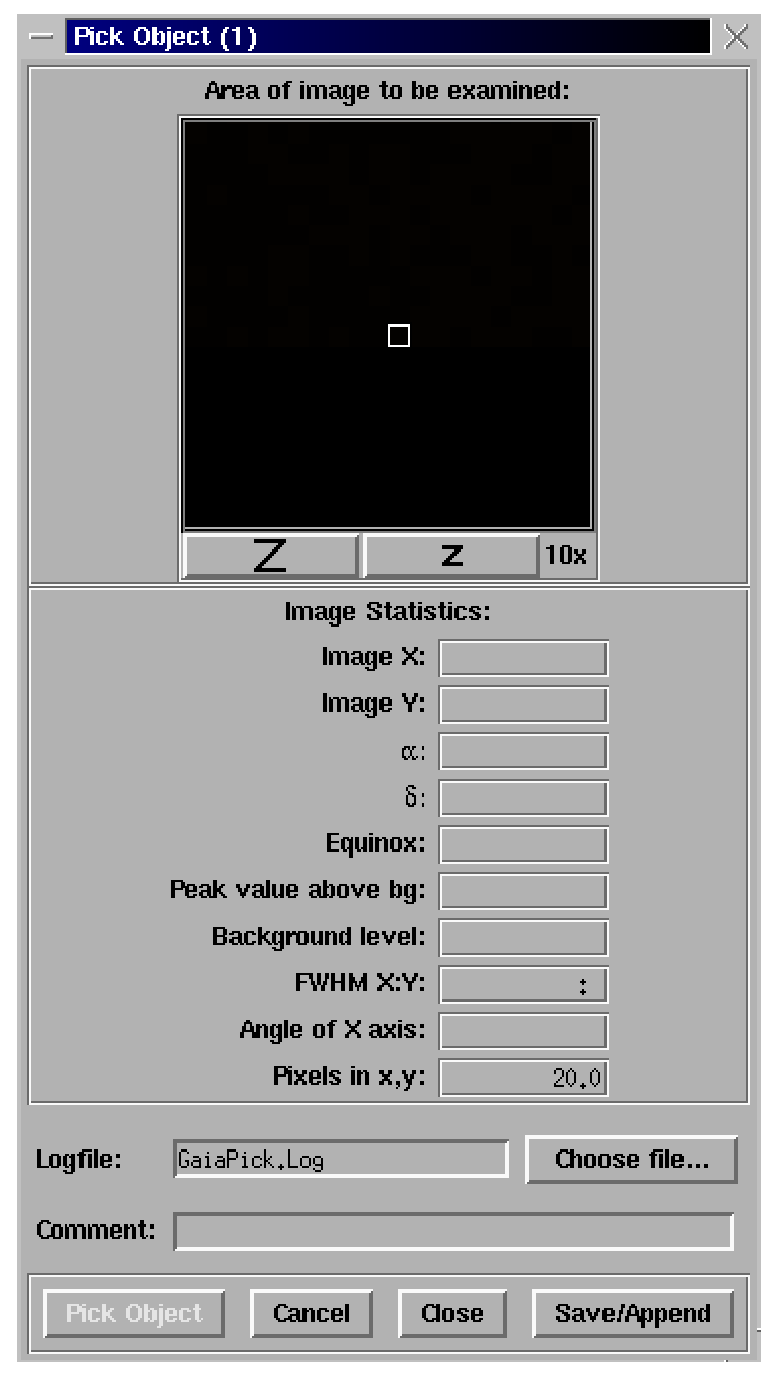
\includegraphics[clip,scale=0.5]{sun223_figures/gaia3.eps}
  \caption{The GAIA object picker dialogue box.}
  \label{fig:gaia3}
  \end{center}
  \end{figure}
\end{latexonly}
\begin{htmlonly}
   \begin{quote}
   \begin{figure}[bhtp]
   \label{fig:gaia3}
   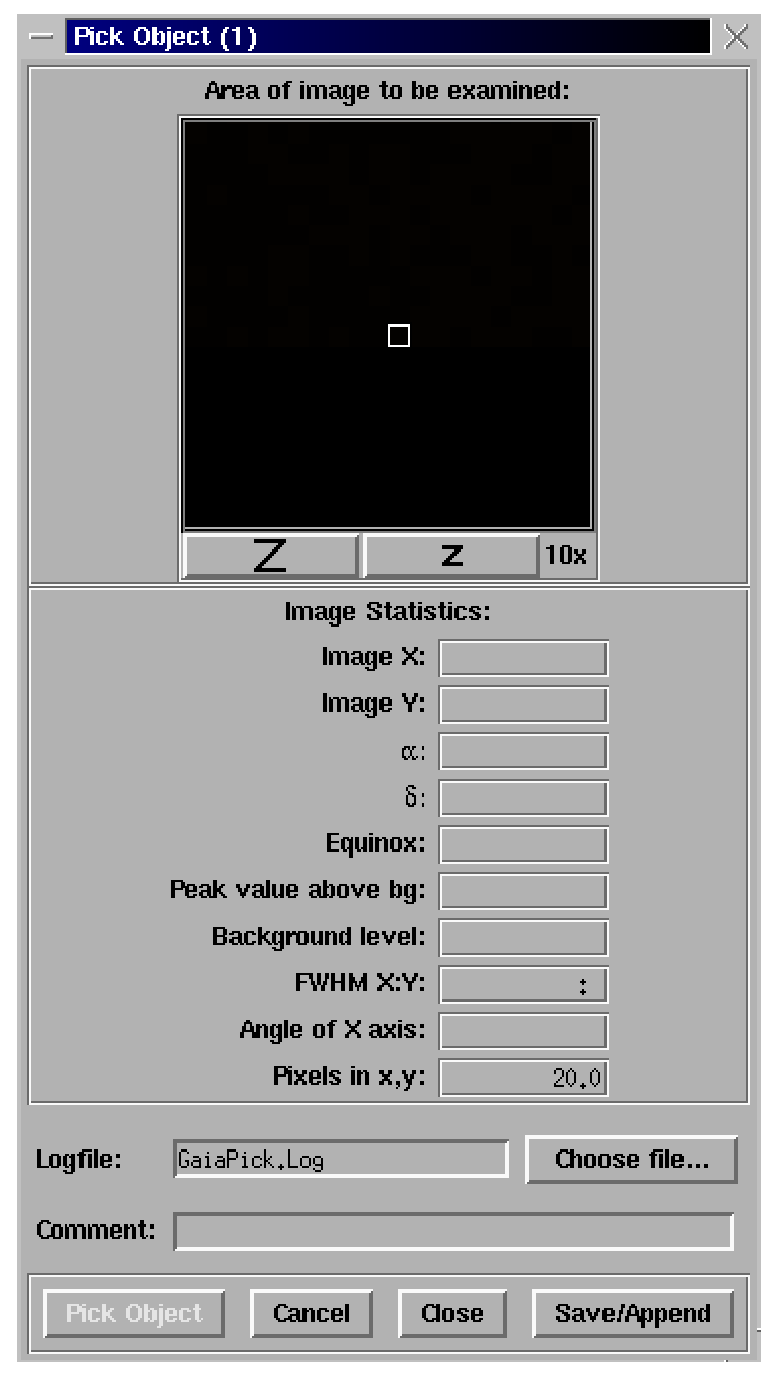
\includegraphics{sun223_figures/gaia3.eps}
   \caption{The GAIA object picker dialogue box.}
   \end{figure}
   \end{quote}
\end{htmlonly}

\item Raise the dialogue box shown in Figure~\ref{fig:gaia2}. You should
find that the pixel co-ordinates of the star have been copied into the
X and Y fields. Click in the \emph{ra} field, and enter the RA of the 
star (eg "12:23:34.1"). Then do the same with the \emph{dec} field. Then
click in the \emph{id} field, and enter an integer value which can be
used to identify the star (for instance, use 1 for your first star, 2 for
your second, etc). The star is now fully specified, so press the
\emph{Enter} button. After confirmation, this will add the object into
the list of reference objects in the dialogue box shown in
Figure~\ref{fig:gaia1}. 

\item All the windows will remain open, so you can continue to enter new
reference stars in the same way. First click on the \emph{Pick Object} 
button in the dialogue box shown in Figure~\ref{fig:gaia3}. Then position
the cursor over a star in the main window, click with the left button, enter 
the RA, DEC and ID values for the star, and press \emph{Enter}.

\item Once you have entered all your reference positions, close the
dialogue boxes shown in Figures~\ref{fig:gaia2} and~\ref{fig:gaia3} by
pressing the \emph{Close} button in each one.

\item Press the \emph{Fit/Test} button in the dialogue box shown in
Figure~\ref{fig:gaia1}. This will calculate the best RA/DEC calibration
given your reference positions. It then uses this calibration to work out
the pixel co-ordinates corresponding to each of your reference positions,
and displays markers in the main image at these pixel co-ordinates. You
should find that they fall on top of the corresponding stars. If they do
not, you have probably entered a bad RA or DEC value. You should correct
the reference positions, and then press the \emph{Fit/Test} button again. To 
correct the reference positions, position the pointer over the erroneous
line in the list of reference positions, and click the left button (the 
selected line will be highlighted). Then click the \emph{Edit} button, the
dialogue box shown in Figure~\ref{fig:gaia2} will re-appear, loaded with
the details of the selected feature. Correct the values, and then press
\emph{Enter}, followed by \emph{Close}. Now you can press \emph{Fit/Test}
again to re-calculate the RA/DEC calibration.

\item Once you are happy with the calibration, press the \emph{Accept}
button. You can now save the RA/DEC calibration by pressing the \emph{File} 
menu button in the main window, and then the \emph{Save as} menu item. Use the
resulting dialog box to save the image (with the RA/DEC calibration) in a
new file. This is most simply done by entering the new file name in the
\emph{Selection} box, and pressing \emph{OK}. Do not worry if a message is
displayed saying that the WCS could only be saved as an AST native
representation.

\end{enumerate}

\section{\label{APP:POLEXT}\xlabel{thepolpackndfextension}The POLPACK NDF Extension}

Figure~\ref{fig:polext} lists the items which may be stored in the
POLPACK extension within a data file. The \htmlref{POLEXP}{POLEXP} and
\htmlref{POLIMP}{POLIMP} applications may be used to transfer these items
to and from a set of corresponding FITS keywords. \htmlref{POLEXT}{POLEXT} 
can be used to set them to explicit values (see \hyperref{here}{section }
{}{SEC:IMPORT}). The contents of the POLPACK extension within an NDF may be 
examined using POLEXT or the \xref{\texttt{hdstrace}}{sun102}{} command.

\begin{latexonly}
  \begin{figure}[tb]
  \begin{center}
  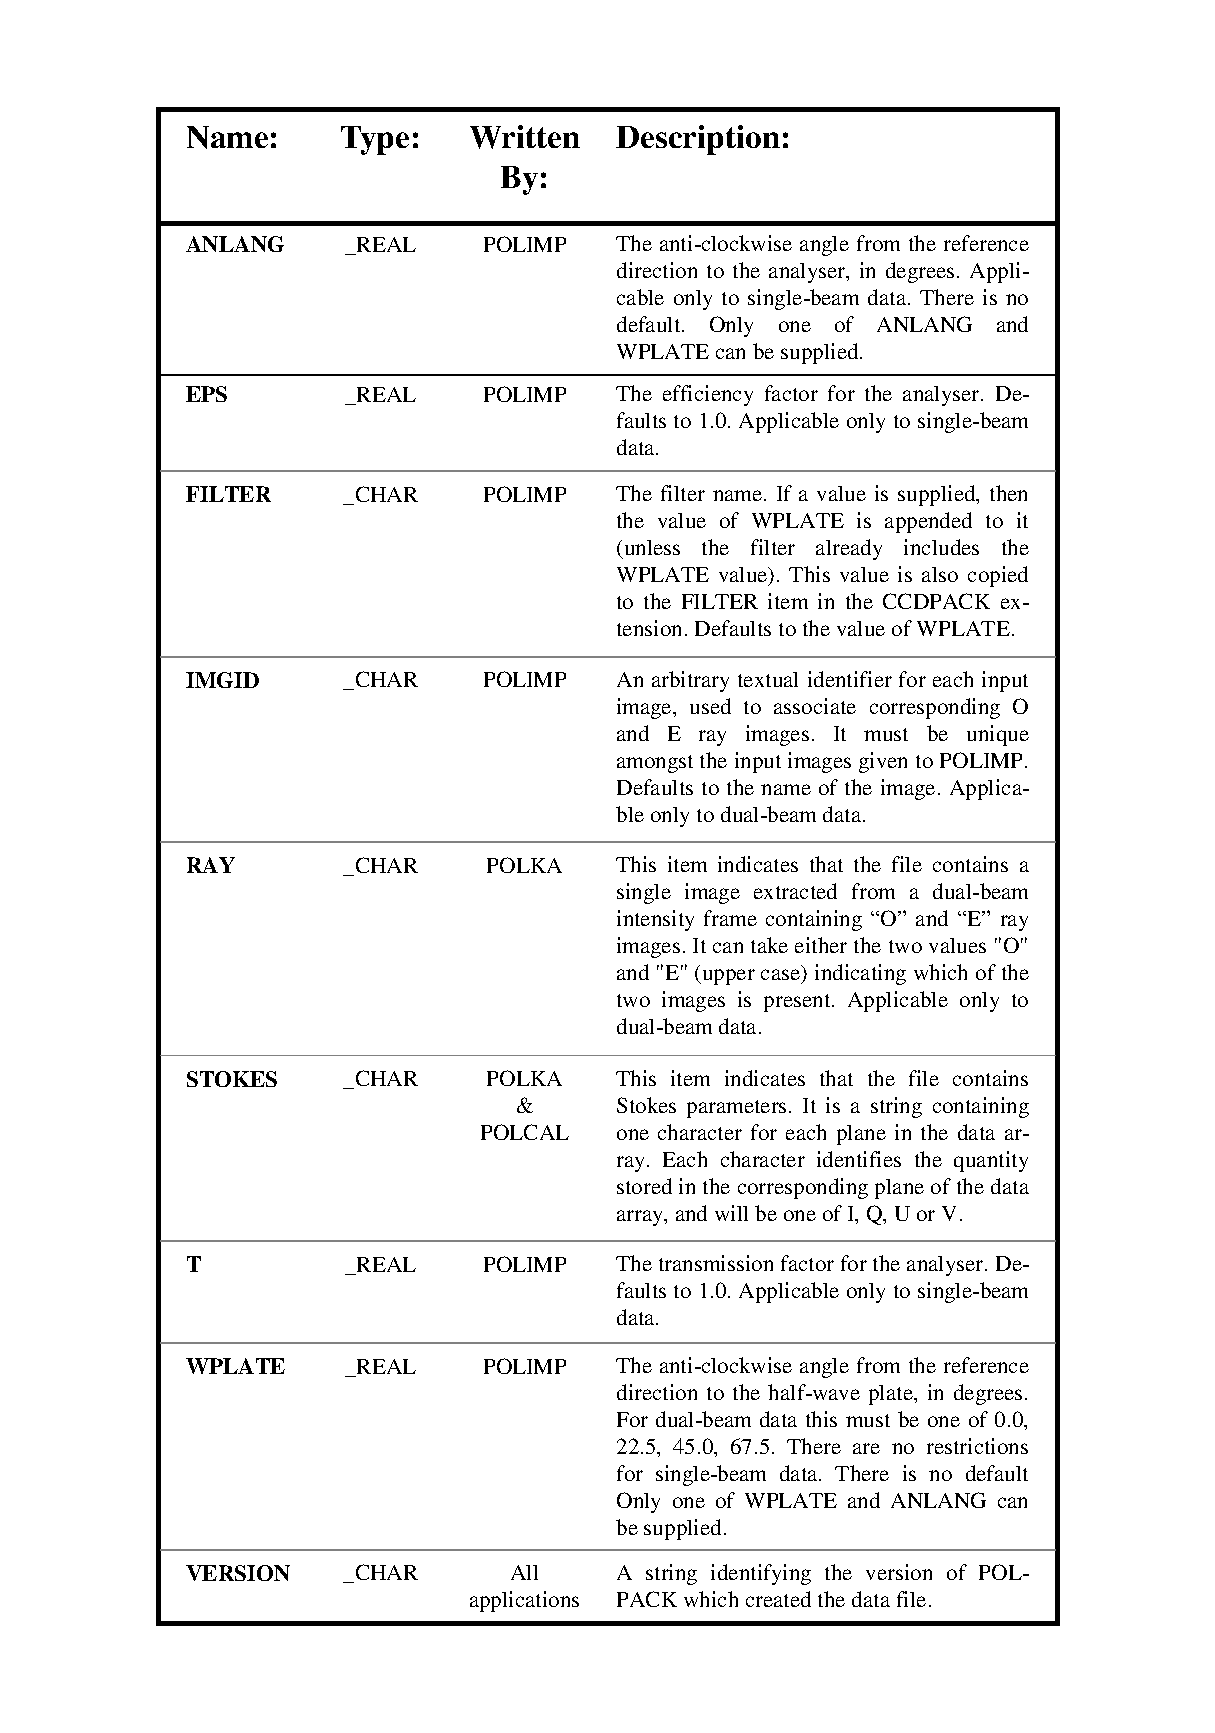
\includegraphics[clip,scale=0.8]{sun223_figures/polext.eps}
  \caption{The allowed items within the POLPACK extension.}
  \label{fig:polext}
  \end{center}
  \end{figure}
\end{latexonly}
\begin{htmlonly}
   \begin{quote}
   \begin{figure}[ht]
   \label{fig:polext}
   \includegraphics{sun223_figures/polext_htx.eps}
   \caption{The allowed items within the POLPACK extension.}
   \end{figure}
   \end{quote}
\end{htmlonly}

\section{\label{APP:HISTORY}History}
This section describes the major changes introduced at each release of
POLPACK.
\subsection{V1.1}
The handling of World Co-ordinate System (WCS) information within POLPACK
has been improved, and is now consistent with WCS handling within KAPPA
V0.13:

\begin{itemize}
\item New sections have been added to SUN/223 describing the use of
RA/DEC calibrations within POLPACK, and how to use GAIA to create them.
\item POLKA now propagates WCS information from input to output. This makes
it possible to retain WCS information throughout an entire POLPACK
reduction. 
\item The COSYS parameter used by POLPLOT has been replaced by FRAME. 
A new parameter called EPOCH has been added to allow the specification of 
an epoch for celestial co-ordinate systems.
\item POLVEC no longer stores a GRID co-ordinate Frame in the output
catalogue (since there is no data grid defined within a catalogue).
\item WCS information can now be read from a FITS or IRAS90 NDF extension
if the NDF has no WCS component.
\item A bug has been fixed which caused POLPLOT to display vectors in 
incorrect positions when annotating the axes with sky coordinates. This bug
was not seen if the vectors were plotted over an existing picture.
\item Catalogues created by POLVEC now inherit the Current coordinate Frame 
from the supplied Stokes cube. Previously the Current Frame was always reset to
pixel coordinates.
\item The vector positions in the catalogue supplied to POLPLOT must now
be given in the Base Frame of the WCS information stored in the catalogue.
\end{itemize}

Other non-WCS related changes include:

\begin{itemize}

\item Vectors produced by POLPLOT no longer intersect the border.

\item If POLKA is used to define a sky region which is then transferred to
a second image, the sky region will be ignored if it does not have an overlap 
with the second image. In this case, a warning is issued and the user is
asked to specify a new sky region for the second image.

\item The handling of graphical styles within POLPLOT (using parameters
STYLE and KEYSTYLE) is now consistent with KAPPA V0.13. In particular:
\begin{enumerate}

\item Defaults for unspecified plotting attributes are now read from file 
\verb+$KAPPA_DIR/style.def+.

\item The values supplied for STYLE and KEYSTYLE are retained and re-used 
on subsequent invocations of POLPLOT (unless new values are given).

\item The size of text produced for a given value of the Size attribute is 
now (roughly) proportional to the size of the picture being used.

\item The default title is now obtained from the TITLE component of
the Stokes cube. Previously it was obtained from the Title attribute of
the WCS information.

\end{enumerate}

\item The vertical spacing between lines in the key produced by POLPLOT can 
now be controlled using the TextLabGap attribute (see parameter KEYSTYLE).

\item A new parameter called MARGIN has been added to POLPLOT. It can be
used to specify the widths of the margins left for axis annotation around
the vector map.

\end{itemize}

\end{document}
